\documentclass[10pt, oneside, a4paper]{article}

\usepackage{estudo_orientado_uff}
\usepackage{graphicx}
\usepackage{hyperref}
\usepackage{caption}
\usepackage{subcaption}
\usepackage{float}
\usepackage{listings}


\usepackage{amsmath,amssymb}

\usepackage{titlesec}
%\setcounter{secnumdepth}{4}
\setcounter{secnumdepth}{5}

\setcounter{tocdepth}{5}

\titleformat{\paragraph}
{\normalfont\normalsize\bfseries}{\theparagraph}{1em}{}
\titlespacing*{\paragraph}{0pt}
{3.25ex plus 1ex minus .2ex}{1.5ex plus .2ex}

\titleformat{\subparagraph}
{\normalfont\normalsize\bfseries}{\thesubparagraph}{1em}{}
\titlespacing*{\subparagraph}{0pt}
{3.25ex plus 1ex minus .2ex}{1.5ex plus .2ex}


\usepackage[spanish]{babel}
\decimalpoint


\newcommand{\titulo}{Cuantificación de la incertidumbre en la clasificación de imágenes y evaluación del impacto de las redes neuronales bayesianas en la clasificación de pacientes con neumonía por COVID-19 en tomografías computarizadas 3D y 2D: un análisis comparativo de rendimiento}
\newcommand{\aluno}{Juan Manuel Liscano Fierro}
\newcommand{\alunoemail}{juan.liscano-f@mail.escuelaing.edu.co}
\newcommand{\orientador}{Hector Javier Hortua Orjuela}
\newcommand{\orientadoremail}{hector.hortua@escuelaing.edu.co}

\renewcommand{\listfigurename}{Lista de Figuras}
\renewcommand{\listtablename}{Lista de Tablas}

\usepackage{enumitem,amssymb}
\newlist{todolist}{itemize}{2}
\setlist[todolist]{label=$\square$}
\usepackage{pifont}
\newcommand{\cmark}{\ding{51}}%
\newcommand{\xmark}{\ding{55}}%
\newcommand{\done}{\rlap{$\square$}{\raisebox{2pt}{\large\hspace{1pt}\cmark}}%
	\hspace{-2.5pt}}
\newcommand{\wontfix}{\rlap{$\square$}{\large\hspace{1pt}\xmark}}

\usepackage{algorithm}
\usepackage{algpseudocode}

\usepackage{listings}
\usepackage{appendix}

\usepackage{adjustbox}

\usepackage{fancyhdr}
\pagestyle{fancy}

%\usepackage[a4paper,width=150mm,top=25mm,bottom=25mm]{geometry}

\begin{document}
	\maketitletwo{\titulo}{\aluno}{\alunoemail}{\orientador}{\orientadoremail}
	
	\newpage
	\section*{Agradecimientos} \label{agradecimientos}
		
	
	\newpage
	\section*{Resumen} \label{resumen}
	La clasificación precisa de la neumonía por COVID-19 en tomografías computarizadas 3D y 2D sigue siendo un desafío en el análisis de imágenes médicas. Aunque las redes neuronales, especialmente las determinísticas, han mostrado promisorios resultados en esta área, carecen de la capacidad para proporcionar una medida de incertidumbre en sus predicciones, un aspecto crucial en la toma de decisiones clínicas. En contraste, las redes neuronales bayesianas ofrecen una interpretación probabilística de sus predicciones, permitiendo cuantificar la incertidumbre y mejorar la toma de decisiones.
	
	\noindent Este proyecto busca comparar la eficiencia de las redes neuronales bayesianas frente a las determinísticas en la clasificación de la neumonía por COVID-19 en tomografías 3D y 2D. Se utilizará un conjunto de datos de 'MosMedData: Chest CT Scans with COVID-19 Related Findings' \cite{mosmed}. Ambos tipos de redes se desarrollarán y entrenarán bajo una arquitectura adecuada, evaluando su rendimiento en precisión, sensibilidad, especificidad y AUC-ROC. 
	
	\noindent Los resultados proporcionarán información valiosa sobre los beneficios potenciales de las redes neuronales bayesianas en imágenes médicas, especialmente en la clasificación de neumonía COVID-19. Al cuantificar la incertidumbre, estas redes pueden mejorar las decisiones clínicas, contribuyendo a los esfuerzos continuos para mejorar el diagnóstico y tratamiento de la neumonía por COVID-19.
	

	\section*{Abstract} \label{abstract}   
	
	Accurately classifying COVID-19 pneumonia in 3D and 2D CT scans remains a significant challenge in the field of medical image analysis. Although neural networks, especially deterministic ones, have shown promising results in this area, they lack the ability to provide a measure of uncertainty in their predictions, a crucial aspect in clinical decision making. In contrast, Bayesian neural networks offer a probabilistic interpretation of their predictions, allowing to quantify uncertainty and improve decision making.
	
	\noindent This research project seeks to compare the efficiency of Bayesian versus deterministic neural networks in the classification of COVID-19 pneumonia in 3D and 2D CT scans. A dataset from 'MosMedData: Chest CT Scans with COVID-19 Related Findings' will be used \cite{mosmed}. Both types of networks will be developed and trained under a suitable architecture, evaluating their performance in terms of accuracy, sensitivity, specificity and AUC-ROC. 
	
	\noindent The results will provide valuable information on the potential benefits of Bayesian neural networks in medical imaging, especially in COVID-19 pneumonia classification. By quantifying uncertainty, these networks can improve clinical decisions, contributing to ongoing efforts to improve the diagnosis and treatment of COVID-19 pneumonia.

	\newpage	
	\tableofcontents
	
	\newpage
	\listoffigures
	\listoftables
	
	
	\newpage
	
	\section*{Información General del Proyecto} \label{info_general}
	
	\begin{itemize}
		\item Modalidad:
		\begin{todolist}
			\item[\done] \textbf{Profundización}
			%\item Write solution
			%\item[\wontfix] profit
		\end{todolist}
		\item Duración del proyecto (meses): 8 Meses
		\item Nombre del estudiante: Juan Manuel Liscano Fierro
		\subitem Programa de maestría al que pertenece: Maestría en Ciencia de Datos
		\item Nombre del director del trabajo de grado: Hector Javier Hortua Orjuela
		\subitem Dedicación del director (horas-semana): 2.5 horas por semana.
		
	\end{itemize}

	\newpage
 	\section{Introducción} \label{introduccion}
	
	En el panorama dinámico de la investigación médica y la inteligencia artificial (IA), la intersección del aprendizaje profundo y las imágenes clínicas se ha convertido en un ámbito fundamental para mejorar las capacidades de diagnóstico. Este proyecto de investigación busca aprovechar las bondades de las redes neuronales tradicionales y de las redes neuronales bayesianas en la clasificación de la neumonía por COVID-19 en tomografías computarizadas 3D y 2D. El objetivo no es sólo mejorar la precisión del diagnóstico sino también explorar el papel vital de la cuantificación de la incertidumbre en el perfeccionamiento de los procesos de toma de decisiones clínicas.
	
	Las redes neuronales, con su capacidad para aprender patrones complejos a partir de vastos conjuntos de datos, han demostrado un éxito notable en diversos ámbitos, incluido el análisis de imágenes médicas. Sin embargo, el paradigma convencional de las redes neuronales a menudo carece de una comprensión matizada de la incertidumbre, un elemento crucial en el diagnóstico médico. Por el contrario, las redes neuronales bayesianas introducen un marco probabilístico que no sólo proporciona predicciones sino que también cuantifica la incertidumbre asociada con esas predicciones, un elemento crítico que a menudo se pasa por alto en los enfoques tradicionales de aprendizaje profundo. Este proyecto busca explorar la eficacia comparativa de las redes neuronales tradicionales y las redes neuronales bayesianas en el contexto de la clasificación de la neumonía COVID-19.
	
	El conjunto de datos es una recopilación de tomografías computarizadas de pulmón humano anonimizadas, que entrelaza la complejidad de las manifestaciones del COVID-19 y el potencial de la tecnología de inteligencia artificial de vanguardia. Estas exploraciones, obtenidas en hospitales médicos de Moscú, Rusia, durante el período comprendido entre el 1 de marzo y el 25 de abril de 2020, capturan una instantánea del impacto de la pandemia en la salud pulmonar. 
	
	Este conjunto de datos, que comprende 424 estudios, cada uno de los cuales corresponde a un paciente único, constituye un ejercicio de clasificación binaria. La tarea que se desarrolla es distinguir entre tejido pulmonar normal (CT-0) y aquellos con diversos grados de afectación de la neumonía por COVID-19 (CT-2 y CT-3). 
	
	La decisión de emplear redes neuronales bayesianas está motivada por el reconocimiento de que la incertidumbre es una faceta inherente de los diagnósticos médicos. No se trata simplemente de hacer predicciones; se trata de comprender la confianza y confiabilidad de esas predicciones. Este proyecto busca destacar la importancia de la incertidumbre en el ámbito de la clasificación de la neumonía COVID-19. Al comparar el enfoque bayesiano con las redes neuronales tradicionales, pretendemos resaltar los beneficios potenciales de un modelo más interpretable, uno que no solo ofrezca predicciones sino que también proporcione información sobre la certeza y las limitaciones de esas predicciones.
	
%	La categorización única de las tomografías computarizadas en cinco clases distintas según el grado de afectación de la neumonía viral agrega granularidad al análisis. Desde la ausencia de signos de neumonía (CT-0) hasta la progresión de opacificaciones en vidrio esmerilado con diversos grados de afectación parenquimatosa, este conjunto de datos resume el espectro de manifestaciones de la COVID-19. Es digno de mención que estas categorías se establecen únicamente en función de los hallazgos radiológicos, divorciados de los resultados de las pruebas de PCR o de la verificación clínica, lo que refleja el escenario del mundo real donde las imágenes son a menudo una herramienta de diagnóstico primaria.
	
	Además, el proyecto incluye un meticuloso proceso de preprocesamiento, que contiene la estandarización de cortes de imágenes, la normalización del valor de los píxeles y la aplicación de técnicas de aumento de datos. Estos pasos son esenciales no sólo para optimizar el entrenamiento del modelo sino también para garantizar la coherencia y confiabilidad del análisis.
	
	
	\subsection{Planteamiento del problema} \label{problema}
	
	% Opción 1	
	%¿Cuál es el impacto de la cuantificación de la incertidumbre proporcionada por \textit{probabilistic deep learning} en la toma de decisiones clínicas y cómo

	% Opción 2	
	%¿Qué ventajas trae la implementación de incertidumbres en los modelos de deep learning para la toma de decisiones clínicas? 
	
	% Opción 3: Enviada en la propuesta.
	%¿Cómo se compara el uso de redes neuronales bayesianas frente a las redes neuronales determinísticas para clasificar con precisión la neumonía causada por el COVID-19 en tomografías computarizadas 3D y 2D del tórax, y cuál es el impacto de la cuantificación de la incertidumbre proporcionada por el enfoque bayesiano en la toma de decisiones clínicas?
	
	% Opción 4
	¿Cómo se compara la implementación de las redes neuronales bayesianas con las redes neuronales determinísticas en su capacidad para clasificar con precisión la neumonía por COVID-19 en tomografías computarizadas 3D y 2D, y cuál es la importancia de cuantificar la incertidumbre asociada a través del enfoque bayesiano para la toma de decisiones clínicas informadas?
	
	La pandemia de COVID-19 atrajo nuevamente la atención de la ciencia sobre el campo de análisis de imágenes médicas, particularmente en el contexto de imágenes pulmonares. Las tomografías computarizadas de tórax se han utilizado ampliamente para ayudar en el diagnóstico y tratamiento de la neumonía por COVID-19, que es una complicación clave de la enfermedad. Sin embargo, clasificar con precisión la neumonía por COVID-19 en las tomografías computarizadas sigue siendo un desafío, particularmente cuando se distingue de otros tipos de neumonía o patologías pulmonares.   
		
	Las técnicas de aprendizaje profundo (Deep Learning), incluidas las redes neuronales, se han mostrado muy prometedoras en el análisis de imágenes médicas, tales como la detección de hemorragias intracerebrales como en \cite{Sharrock2021} y \cite{Chang1609} , incluso en el diagnóstico de la neumonía y afecciones pulmonares por COVID-19 \cite{nn_lung_lesions}. Las redes neuronales determinísticas se han utilizado para clasificar la neumonía por COVID-19 en tomografías computarizadas con buenos resultados, pero no tienen en cuenta la incertidumbre inherente a las imágenes médicas y el diagnóstico. Las redes neuronales bayesianas, por otro lado, pueden proporcionar una interpretación probabilística de sus predicciones, lo que puede ser útil para los médicos en los procesos de toma de decisiones.
	
	El uso de técnicas de aprendizaje profundo en imágenes médicas se ha vuelto cada vez más importante en los últimos años, ya que tienen el potencial de mejorar la precisión del diagnóstico, reducir la variabilidad entre observadores y mejorar la eficiencia de los flujos de trabajo clínicos como en \cite{LUNDERVOLD2019102} y \cite{doi:10.1146/annurev-bioeng-071516-044442}. Por ejemplo, un estudio de \cite{McKinney2020} demostró que los algoritmos de aprendizaje profundo podían detectar con precisión el cáncer de seno a través de imágenes, con un rendimiento similar al de los radiólogos experimentados. En otro estudio, \cite{Ardila2019} demostró que los algoritmos de aprendizaje profundo pueden detectar con precisión el cáncer de pulmón en tomografías computarizadas, donde habla del potencial en los modelos de aprendizaje profundo para aumentar la precisión y la adopción de las pruebas de detección del cáncer de pulmón en todo el mundo. Creando una oportunidad para optimizar el proceso de selección a través de la asistencia informática y la automatización.
	
	Existen varias técnicas diferentes que se pueden utilizar en el análisis de imágenes médicas, incluidas las redes neuronales convolucionales, las redes neuronales recurrentes y los modelos generativos. Cada una de estas técnicas tiene sus propias fortalezas y debilidades, y la elección de la técnica dependerá de la aplicación y el conjunto de datos específicos. Por ejemplo, las redes neuronales convolucionales son particularmente efectivas en la extracción de características en imágenes 2D o 3D, mientras que las redes neuronales recurrentes son útiles para analizar datos de series temporales.
	
	Las redes neuronales bayesianas representan un enfoque particularmente prometedor en este campo, ya que pueden proporcionar una medida de incertidumbre que falta en las redes neuronales determinísticas. La cuantificación de la incertidumbre es esencial en la toma de decisiones clínicas, ya que permite a los médicos emitir juicios informados sobre la fiabilidad de las predicciones diagnósticas y ajustar los planes de tratamiento en consecuencia. 
	
	% tener un modelo más interpreativo, donde ya sabe lo que no sabe. 	
	% facilitar la interpretaciónde las predicciones arrojadas por los modelos de RN.
	% papel que toma la incertidumbre.
	% Comentar la ayuda sobre los riadologos	
	
	Medir y calibrar las incertidumbres del modelo es fundamental en la toma de decisiones clínicas, ya que estas proporcionan información valiosa sobre la fiabilidad y confianza de las predicciones, identificando áreas en las que las predicciones del modelo pueden ser poco fiables o inconsistentes, y así mismo permitiendo comprender mejor las limitaciones del modelo y los posibles errores. Esto es especialmente importante en el caso de la neumonía por COVID-19, donde la clasificación errónea puede tener graves consecuencias para el tratamiento del paciente. Al mejorar la precisión y confiabilidad de los modelos de clasificación, podemos mejorar la calidad de la atención y respaldar la toma de decisiones clínicas. Esta información es crucial para que los médicos y radiólogos tomen decisiones informadas sobre el diagnóstico del paciente. 
	
	Comprender la incertidumbre asociada con las predicciones ayuda a identificar casos en los que el modelo sea más incierto y que pueda ser necesaria una mayor investigación o una segunda opinión, asegurando que los pacientes reciban la atención adecuada y minimizando el riesgo de diagnóstico erróneo, promoviendo un enfoque más transparente y responsable para utilizar modelos de aprendizaje profundo en entornos clínicos.
		
	Al comparar las redes neuronales bayesianas con las redes neuronales tradicionales o determinísticas, podemos valorar los avances y los beneficios potenciales que aportan los enfoques bayesianos al campo del análisis de imágenes médicas. Esta investigación tiene el potencial de contribuir al desarrollo de modelos de diagnóstico más confiables.
	
	En conclusión, el uso de redes neuronales bayesianas en imágenes médicas representa una vía prometedora para mejorar la precisión y confiabilidad de las predicciones diagnósticas, particularmente en el contexto de la clasificación de neumonía por COVID-19 en tomografías computarizadas 3D y 2D. Al proporcionar una medida de incertidumbre, las redes neuronales bayesianas pueden mejorar la toma de decisiones clínicas y facilitar el desarrollo de planes de tratamiento más personalizados. Por ello se necesita más investigación en esta área para evaluar el rendimiento de las redes neuronales bayesianas en comparación con las redes neuronales determinísticas y para evaluar su impacto potencial en la práctica clínica.
	
	
	\subsection{Objetivos}
	
	
	\subsubsection{General}
	\begin{itemize}
		\item Evaluar el impacto de la cuantificación de la incertidumbre proporcionada por las redes neuronales bayesianas en la clasificación de la neumonía por COVID-19 en tomografías computarizadas 3D y 2D.  
		
		%\item Comparar la eficiencia de las redes neuronales bayesianas frente a las redes neuronales determinísticas en la clasificación de la neumonía por COVID-19 en tomografías computarizadas 3D y 2D, y evaluar el impacto de la cuantificación de la incertidumbre proporcionada por el enfoque bayesiano en la toma de decisiones clínicas.
		
		
	\end{itemize}
	
	\subsubsection{Específicos}
	\begin{itemize}
		
		% \item implementar modelos de redes bayesianas que proveen una correcta calibración de sus incertidumbres.
		
		% \item incorporar metodologias para la cuantificación de la incertidumbre alea y epi en las redes bayesianas 
		
		\item Entrenar redes neuronales determinísticas y bayesianas optimizadas para detectar neumonía por COVID-19 en tomografías computarizadas 2D y 3D a través del paquete TensorFlow.
		
		\item Incorporar una metodología adecuada para la calibración y cuantificación de la incertidumbre aleatoria y epistémica en diferentes redes neuronales bayesianas asociadas a la tarea de clasificación.%, y analizar las ventajas que conlleva la implementación de estos algoritmos en la toma de decisiones.
		
		\item Estudiar y evaluar el desempeño de las redes neuronales determinísticas y bayesianas en términos de precisión, sensibilidad, especificidad y área bajo la curva ROC (AUC-ROC).
		
		\item Implementar métodos para la calibración de las incertidumbres encontradas en cada uno de los modelos estocásticos. 
		
	\end{itemize}

	\subsection{Alcance y Limitaciones} \label{alcance_limitaciones}

	\subsubsection{Alcance}
	
	\begin{itemize}
		\item Este proyecto de investigación se centra en la implementación y comparación de redes neuronales tradicionales y redes neuronales bayesianas para la clasificación de la neumonía por COVID-19 en tomografías computarizadas 3D y 2D. El modelo está diseñado específicamente para clasificar anomalías CT-0 como indicativas de ausencia de neumonía, y combina las etiquetas CT-2 y CT-3 como indicativas de la presencia de manifestaciones características de neumonía por COVID-19. Este enfoque específico tiene como objetivo optimizar el rendimiento del modelo para escenarios de clasificación clínicamente relevantes. El alcance incluye además el preprocesamiento del conjunto de datos, el desarrollo de modelos, el entrenamiento y la evaluación. Por último, el proyecto busca explorar la importancia de la cuantificación de la incertidumbre proporcionada por los enfoques bayesianos en la toma de decisiones clínicas.
	\end{itemize}

	\subsubsection{Limitaciones}

	\begin{itemize}
%		\item Capacidad de procesamiento: Los recursos computacionales disponibles, particularmente la capacidad de procesamiento en la máquina virtual, imponen limitaciones a la escalabilidad de ciertos aspectos del proyecto. Específicamente, las limitaciones de capacidad restringen la expansión del tamaño de los lotes (batches) durante el entrenamiento, lo que podría afectar la eficiencia de la convergencia del modelo y la exploración de conjuntos de datos más grandes.
		
		\item Capacidad de procesamiento: Los recursos computacionales disponibles, particularmente la capacidad de procesamiento en la máquina virtual, imponen limitaciones a la escalabilidad de ciertos aspectos del proyecto. Específicamente, las limitaciones de capacidad restringen la expansión de los tamaños de lote (\textsl{batches}) durante el entrenamiento, lo que podría afectar la eficiencia de la convergencia del modelo y la exploración de conjuntos de datos más grandes. Esto a su vez influyó en la decisión de centrarse en un subconjunto de clasificaciones de tomografías computarizadas para garantizar un entrenamiento y evaluación eficientes del modelo.

		\item Complejidad del modelo: debido a limitaciones de recursos, la complejidad de las arquitecturas de redes neuronales puede ser limitada. Esta limitación podría afectar la profundidad y amplitud de las características aprendidas por los modelos, afectando potencialmente su rendimiento en comparación con arquitecturas más complejas.
		
		\item Especificidad del conjunto de datos: el conjunto de datos utilizado en este proyecto de investigación se limita a tomografías computarizadas de pulmón humano anonimizadas con hallazgos relacionados con COVID-19, obtenidos de hospitales médicos en Moscú, Rusia, durante un período de tiempo específico. Si bien este conjunto de datos proporciona información valiosa sobre la clasificación de la neumonía por COVID-19, es posible que su alcance no capture completamente la diversidad de casos observados a nivel mundial o en diferentes entornos de atención médica.	
		
		\item Relevancia clínica: La decisión de priorizar las clasificaciones CT-0, CT-2 y CT-3 se alinea con la importancia clínica de distinguir entre ausencia y presencia de manifestaciones características de neumonía en pacientes con COVID-19. Las clasificaciones CT-1 y CT-4, si bien son importantes, pueden representar escenarios relativamente raros o atípicos que son menos prevalentes en el conjunto de datos o menos relevantes clínicamente para la tarea de diagnóstico específica en cuestión.
		
		\item Generalizabilidad: Los hallazgos y conclusiones extraídas de esta investigación pueden ser específicas del conjunto de datos y la configuración experimental utilizada. La generalización de los resultados a poblaciones más amplias o conjuntos de datos con diferentes características debe hacerse con cautela, considerando posibles variaciones en la demografía de los pacientes, los protocolos de imágenes y las manifestaciones de la enfermedad.
		
		\item Interpretabilidad: si bien las redes neuronales bayesianas ofrecen una cuantificación mejorada de la incertidumbre, la interpretabilidad de las predicciones de los modelos aún puede plantear desafíos. Comprender los factores subyacentes que impulsan las decisiones sobre modelos, particularmente en tareas complejas de imágenes médicas, sigue siendo un área de investigación en curso.
		
		\item Factores externos: los factores externos, como las variaciones en la calidad de la imagen, los artefactos y las anotaciones, pueden introducir ruido o sesgos en el análisis, lo que podría influir en el rendimiento y la interpretabilidad de los modelos.
		
		\item Consideraciones éticas: Durante todo el proceso de investigación se deben reconocer y abordar las consideraciones éticas relacionadas con el uso responsable de la IA en la atención sanitaria, incluidas las cuestiones de sesgo, equidad y transparencia.
	\end{itemize}

					
	\section{Fundamentación Teórica} \label{marco_teorico}
	
	% Modelo determinístico es aquel donde se supone que los datos se conocen con certeza, es decir, se supone que cuando el modelo sea analizado se tiene disponible toda la información necesaria para la toma de decisiones. Es un modelo matemático donde las mismas entradas producirán invariablemente las mismas salidas (no se contempla la existencia del azar ni el principio de incertidumbre)
	
	% Modelo estocástico o probabilístico, es aquel en donde algún elemento no se conoce con anticipación, incorporando la incertidumbre. Es estocástico cuando al menos una variable del mismo es tomada como un dato al azar y las relaciones entre las variables se toman medio de funciones probabilísticas. 
	
	\subsection{Redes Neuronales Profundas} \label{dnn}
	
	En los últimos años, las redes neuronales profundas (DNNs, por sus siglas en inglés) se han convertido en modelos de alto rendimiento. Estas redes se componen de múltiples capas de nodos de procesamiento o neuronas interconectadas. Con esa arquitectura son capaces de aprender representaciones complejas de datos de entrada a través de un proceso conocido como entrenamiento, que implica ajustar los pesos de las conexiones entre las neuronas para minimizar el error entre la salida predicha y la salida real. Estas neuronas procesan los datos de entrada de una manera particular; la primera capa de una DNN es la capa de entrada, que toma los datos de entrada sin procesar y los transforma en un conjunto de características que luego procesan las capas posteriores. La salida de la capa final es la salida prevista de la red, es decir, la cantidad de neuronas va a depender del objetivo. El proceso de entrenamiento generalmente se lleva a cabo utilizando el algoritmo de descenso de gradiente estocástico (SGD, por sus siglas en inglés), donde los pesos se actualizan en pequeños incrementos en función del gradiente de error calculado con respecto a un conjunto de entrenamiento. Este proceso se repite para varias sub-muestras durante el entrenamiento hasta que el promedio de la función objetivo deja de decrecer y se le llama estocástico porque cada una de estas sub-muestras da una estimación ruidosa del promedio del gradiente de todos los ejemplos \cite{LeCun2015}. Luego del entrenamiento, el modelo se evalúa en un set de datos diferente que comúnmente se denomina set de validación o testeo, y así finalmente se evalúa la habilidad del modelo para generalizar las predicciones. 
	
	Las DNN se han convertido en la técnica de vanguardia para una amplia gama de aplicaciones, incluido el reconocimiento de voz, detección de objetos en imágenes, entre otros casos como lo mencionan en \cite{LeCun2015}. Uno de los factores clave que han contribuido a su éxito es la disponibilidad de conjuntos de datos a gran escala y potentes recursos informáticos que permiten el entrenamiento de arquitecturas profundas con millones de parámetros.
	
	Matemáticamente, en un vector de entrada $x = [x_{1}, x_{2}, x_{3}, ... , x_{d}]$ de dimensión $d$, la operación realizada por cada neurona se representa por
	

	\begin{equation} 
		f(\sum_{i = 1}^{d} W_{i} x_{i} + b),
		\label{eq:1}
	\end{equation}


	donde $W_{i}$ es el vector que contiene los pesos de cada neurona y multiplica con cada una de las entradas en $x$, $b$ corresponde al término de sesgo, un parámetro único que permite ajustar la salida junto con la suma ponderada, estos se conocen como \textsl{learnable parameters}, y por último $f()$ corresponde a la función de activación.

	En resumen, las DNN son una clase potente y versátil de modelos de aprendizaje automático que han revolucionado muchos campos de la investigación y la industria. Su éxito se debe a su capacidad para aprender representaciones complejas de datos de entrada y su escalabilidad a grandes conjuntos de datos y espacios de entrada de gran dimensión.

	
	\subsubsection{Redes Neuronales Convolucionales} \label{cnn}
			
	Las redes neuronales convolucionales (CNN, por sus siglas en inglés) son un tipo especializado de DNN que han sido particularmente exitosas en tareas de reconocimiento de imágenes dentro del campo de la salud, como en la detección de cáncer de hueso conocido como osteosarcoma \cite{GAWADE2023100153} y otros estudios importantes como la detección de la enfermedad de Alzheimer trabajado en \cite{DESILVA2023100091}. La innovación clave de las CNN es el uso de capas convolucionales, que aplican un conjunto de filtros de aprendizaje a la imagen de entrada para extraer características locales como bordes y texturas. Estos filtros son generalmente de un tamaño pequeño (ej. 3x3 o 5x5) y se aplican a la imagen de entrada en una forma de ventana que se desliza por toda la imagen como lo ilustra la sección de extracción de características (\textsl{Feature Extraction}) en la Fig.(~\ref{fig:cnn_1}). La salida de la capa convolucional luego pasa a través de una función de activación no lineal, como por ejemplo la unidad lineal rectificada (ReLU), para introducir no linealidades en el modelo. 
	
	Estas capas convolucionales tienen varias ventajas importantes sobre las capas totalmente conectadas, que se utilizan en las redes neuronales. En primer lugar, las capas convolucionales tienen menos parámetros que las capas completamente conectadas, lo que reduce el riesgo de sobreajuste y permite el entrenamiento de arquitecturas más profundas. En segundo lugar, las capas convolucionales aprovechan la estructura espacial de la imagen de entrada, lo que permite la detección de características invariantes a la traslación. Esto significa que un filtro que detecta una característica particular en una parte de la imagen también puede detectar la misma característica en otra parte de la imagen, incluso si se ha trasladado o girado.
	Además de las capas convolucionales, las CNN también suelen incluir capas de agrupación (\textsl{pooling}), que se utilizan para reducir la dimensionalidad espacial de los mapas de características producidos por las capas convolucionales y son útiles para aumentar la eficiencia de la red. Las capas de agrupación agregan las activaciones de los elementos vecinos en el mapa de características, lo que reduce la cantidad de parámetros y ayuda a reducir el sobreajuste. Los tipos más comunes de agrupación son la agrupación máxima y promedio, que toma el valor de activación máximo o promedio en una vecindad local del mapa de características.
	
	En resumen, las capas convolucionales son un bloque de construcción fundamental de las redes neuronales convolucionales y son esenciales para la extracción efectiva de características en las tareas de reconocimiento de imágenes. Aprovechan la estructura espacial de la imagen de entrada y tienen menos parámetros que las capas completamente conectadas, lo que las hace muy adecuadas para arquitecturas profundas y reduce el riesgo de sobreajuste.
	
	\begin{figure}[H]
		\includegraphics[scale=0.4]{cnn.png}
		\caption{{\small Arquitectura de una RNN compuesta por capas convolucionales. Tomada de \href{https://developersbreach.com/convolution-neural-network-deep-learning/}{developersbreach}}}
		\label{fig:cnn_1}
	\end{figure}
	
	Estas arquitecturas convolucionales son muy comunes en CNN como AlexNet \cite{AlexNet}, VGG Net \cite{VGG16}, y ResNet \cite{resnet}.
	
	\subsubsection{Capas de Normalización y Pooling en CNN}
	
	En las redes neuronales convolucionales (CNN), las capas pooling desempeñan un papel crucial en la reducción de las dimensiones espaciales de los mapas de características \footnote{Los mapas de características, también conocidos como mapas de activación, son la salida de capas convolucionales en una red neuronal convolucional (CNN).} generados por las capas convolucionales, reduciendo así la complejidad computacional y controlando el sobreajuste. Además, con frecuencia se emplean capas de normalización por lotes para acelerar el proceso de entrenamiento y mejorar la estabilidad de la red.
	
	\begin{itemize}
		\item Capas GlobalAveragePooling3D y 2D: La agrupación promedio global es una técnica que se utiliza para reducir la muestra de los mapas de características obtenidos de capas convolucionales. En esta capa, cada mapa de características se promedia en todas sus dimensiones espaciales, lo que da como resultado un valor único por mapa de características. Estas capas ayudan a reducir las dimensiones espaciales de los mapas de características y al mismo tiempo retiene información importante. Es particularmente útil para reducir el sobreajuste al resumir todo el mapa de características en un solo valor.
		\item GlobalMaxPooling3D y 2D: De manera similar a la agrupación promedio global, la agrupación máxima global es otra técnica de reducción de resolución utilizada en las CNN. En esta capa, el valor máximo dentro de cada mapa de características se extrae en todas las dimensiones espaciales. La agrupación máxima global resalta las características más importantes dentro de cada mapa de características y descarta información irrelevante.
		\item MaxPool3D y 2D: La agrupación máxima es una técnica de reducción de resolución local que divide los mapas de características de entrada en regiones que no se superponen y retiene solo el valor máximo dentro de cada región. Esta capa ayuda a reducir las dimensiones espaciales de los mapas de características y al mismo tiempo preserva las características más dominantes. 
		\item BatchNormalization: La normalización por lotes es una técnica utilizada para normalizar las activaciones de cada capa en una red neuronal ajustando y escalando las activaciones para que tengan media cero y varianza unitaria. Esta capa ayuda a estabilizar y acelerar el proceso de entrenamiento al reducir el cambio de covariables interno. Al normalizar las activaciones, la normalización por lotes permite una convergencia más fluida y rápida durante el entrenamiento, lo que conduce a un mejor rendimiento y a la generalización del modelo.
	\end{itemize}
	
	% \subsubsection{Propagación inversa de errores}	\label{backpropagation}


	
	\subsection{Redes Neuronales Bayesianas} \label{bnn}
	
	Las redes neuronales bayesianas (BNN, por sus siglas en inglés) son un tipo de red neuronal que incorpora la teoría de la probabilidad bayesiana en el proceso de entrenamiento e inferencia. A diferencia de las redes neuronales deterministas, que generan una predicción fija dado un conjunto de entradas, las BNN generan una distribución de probabilidad sobre posibles predicciones (Fig(~\ref{fig:bnn_1}) ilustra de forma general cómo se produce una estimación bajo una red neuronal bayesiana). Esto permite modelar la incertidumbre epistémica, que es la incertidumbre asociada a los parámetros del modelo (esto puede imaginarse como la dispersión de la distribución a posteriori de los pesos $p(w|D)$, en la que una distribución posterior más plana refleja una mayor incertidumbre epistémica, mientras que una distribución posterior con picos refleja una menor incertidumbre epistémica), y la incertidumbre aleatoria, que es la aleatoriedad inherente a los datos, en donde dados unos datos de entrada y los parámetros de pesos fijos, una incertidumbre elevada significa que tenemos una estimación volátil o ruidosa de su predicción (para la regresión) o no sabemos a qué clase pertenece (para la clasificación). Una incertidumbre aleatoria alta sugiere que no tenemos suficiente información para predecir el valor de salida para una entrada con parámetros de peso fijos, debido a variables no observadas o latentes que el modelo no puede capturar \cite{chai2018uncertainty}.
	
	\cite{chai2018uncertainty} habla sobre la importancia de descomponer la incertidumbre predictiva argumentando que las incertidumbres aleatorias y epistémicas nos hablan sobre las diferentes facetas de un valor de entrada (input). Una incertidumbre epistémica alta sugiere que el valor de entrada es un valor atípico en relación con la distribución de entrenamiento, y se puede reducir recomiendo más datos de entrenamiento cerca de la región de evaluación, de tal forma que en el caso de contar con datos infinitos, esta incertidumbre se reduzca a cero (es decir, si conocemos todos los datos del universo, confiamos en la función que asigna la entrada a la salida, y por tanto la distribución de pesos se convierte en un pico), pero más datos no ayudan a la incertidumbre aleatoria; para reducirla, se necesitan conocimientos sobre variables no observadas a través de características adicionales o mediciones más refinadas. En la práctica, estas mediciones no suelen estar disponibles, por lo que no siempre es posible reducir la incertidumbre aleatoria.

	
	\begin{figure}[H]
	\includegraphics[scale=0.3]{bnn.png}
	\caption{{\small Ilustración de la generación de una predicción a partir de una red neuronal bayesiana mediante el muestreo de Monte Carlo.
	Una red neuronal estándar (A, arriba a la izquierda) tiene un peso para cada una de sus conexiones $(w*)$, ajustadas a través del conjunto de entrenamiento y utilizada para generar una predicción para un ejemplo de prueba. Una red neuronal bayesiana (B, abajo a la izquierda) tiene, en cambio, una distribución posterior para cada peso, parametrizada por teta ($q_{\theta}(w)$). El proceso de entrenamiento comienza con una distribución previa asignada para cada peso y devuelve una distribución posterior aproximada. En el momento de la prueba (C, derecha), se extrae una muestra $w_{1}$ (rojo) de la distribución a posteriori de los pesos y la red resultante se usa para generar una predicción $p(y|x,w_{1})$ para un ejemplo x. Se puede hacer lo mismo con las muestras $w_{2}$ (azul) y $w_{3}$ (verde), lo que arroja predicciones $p(y|x,w_{2})$ y $p(y|x,w_{3})$, respectivamente. Las tres redes se tratan como un conjunto y se promedian sus predicciones. Tomada de \href{https://www.researchgate.net/publication/336608788_Knowing_What_You_Know_in_Brain_Segmentation_Using_Bayesian_Deep_Neural_Networks}{\cite{brain_segmentation}}}}
	\label{fig:bnn_1}
	\end{figure}
	
	Los BNN usan distribuciones a priori sobre los pesos de la red y aprenden distribuciones a posteriori $p(w/D)$ usando la regla de Bayes: $ p(w|D) \sim p(D|w)p(w)$, donde $p(D|w)$ denota la función de verosimilitud que representa la probabilidad de los datos observados $D$ dado los pesos $w$, y $p(w)$ que representa la distribución a priori de los pesos. La distribución a posteriori representa la incertidumbre en los pesos dados los datos observados $D = (X, Y)$ normalmente se aproxima mediante métodos de inferencia variacional \cite{chai2018uncertainty, heek2018well} o cadena de Markov Monte Carlo (MCMC) \cite{neal2012bayesian}. Luego, la distribución a posteriori se usa para hacer predicciones tomando la esperanza del ouput sobre la distribución. Una vez realizado el cálculo de la distribución a posteriori, la distribución de probabilidad de un ejemplo nuevo de prueba $x^{*}$ puede determinarse por

	\begin{equation} \label{eq:posterior_test_example}
	p(y^{*} | x^{*}, D) = \int_{w}^{} p(y^{*} | x^{*}, w) p(w|D) dw,
	\end{equation}	
	
	
	donde $p(y^{*} | x^{*}, w)$ es la distribución predictiva posterior correspondiente al set de pesos. 
	Una ventaja de las BNN es que pueden proporcionar predicciones más sólidas y confiables al tener en cuenta la incertidumbre en los datos y el modelo. Esto es particularmente útil en aplicaciones donde las predicciones incorrectas o inciertas pueden tener consecuencias graves, como diagnósticos médicos o pronósticos financieros. Otra ventaja es que las BNN pueden proporcionar una medida de incertidumbre para cada predicción, que se puede usar para guiar la toma de decisiones o para identificar áreas donde se necesitan más datos o refinamiento del modelo.
	
	Sin embargo, también existen algunos desafíos asociados con el uso de BNN. Un desafío es que pueden ser computacionalmente costosos para entrenar y evaluar. Otro desafío es que pueden ser más difíciles de interpretar en términos matemáticos que las redes neuronales determinísticas, ya que el resultado es una distribución de probabilidad en lugar de una sola predicción. Además, elegir distribuciones previas y métodos de inferencia apropiados puede ser un desafío y puede tener un impacto significativo en el rendimiento del modelo.
	
	En resumen, las redes neuronales bayesianas son un enfoque prometedor para modelar la incertidumbre en las redes neuronales y pueden brindar predicciones más sólidas y confiables en ciertas aplicaciones. Sin embargo, también presentan algunos desafíos y requieren una cuidadosa consideración de las distribuciones a priori y los métodos de inferencia apropiados.
	
	\subsubsection{Distribución de pesos $w$ a posteriori}
	% Tesis Chai
	
	\sloppy  Dado un set de datos de entrenamiento con tamaño N con entradas $x$ y salidas $y$ denominado $D = \{(x^{(1)},y^{(1)}),(x^{(2)},y^{(2)}),...,(x^{(N)},y^{(N)})\} $, una red neuronal bayesiana (BNN) puede ajustar la distribución a posteriori sobre los pesos de la red, $p(w|D)$. Como se ha mencionado, $w$ consolida todos los pesos sobre las $L$ capas en la red: $w = \{w_{l}\}^{L}_{l=1}$. Esta distribución representa qué tan probable es un determinado set de pesos después de ver los datos de entrenamiento, en vez de una estimación puntual de los pesos en las DNNs. Una aplicación directa de la regla de bayes produce 
	
	\begin{equation} \label{eq:2}
	p(w|D) = \frac{p(D|w) p(w)}{p(D)},
	\end{equation}
	
	en el numerador, el primer término $p(D|w)$ refleja la verosimilitud de los datos de entrenamiento dado un determinado set de pesos $w$. Asumiendo que cada punto de datos de entrenamiento es independiente, esta cantidad se convierte en el producto de verosimilitudes para cada punto de entrenamiento individual

	\begin{equation} \label{eq:3}
	p(D|w) = \prod_{n=1}^{N} p(y^{(n)} | w,x^{(n)}).
	\end{equation}
	
	Las tareas de clasificación pueden usar las predicciones softmax de la red neuronal directamente como la verosimilitud: $p(y = c |w,x) = f^{w}(x)^{c}$, donde $c$ es la verdadera clase del input, y las predicciones softmax para cada clase $f^{w}(x)^{c}$  están normalizadas para ser mayores a 0 y sumar 1 \cite{chai2018uncertainty}.
	
	El segundo término del numerador, $p(w)$ es la distribución a priori sobre los pesos. Refleja una creencia sobre la distribución de los pesos $w$ sin ver ningún dato. Un ejemplo de distribución a priori es la distribución normal. Los dos términos del numerador son tratables al momento de calcular un determinado set de $w$. Sin embargo, el problema de lograr la distribución posterior es el denominador $p(D)$. Calcular $p(D)$ implica marginar todas las configuraciones de los pesos

	\begin{equation} \label{eq:4}
	p(D) = \int p(D|w) p(w) dw.
	\end{equation}
	
	En muchos modelos, esta integral es intratable, motivando la necesidad de aproximaciones de la a posteriori. Métodos de muestreo, como Metropolis Hastings o Hamiltonian Monte Carlo,
	producen estimaciones no sesgadas de la verdadera a posteriori, pero pueden tardar en converger. Un enfoque alternativo es la inferencia variacional, en la que la verdadera distribución a posteriori se aproxima con una distribución variacional más simple \cite{blei2017variational, jordan1999introduction}. Esta aproximación está sesgada, pero suele ser más rápida que los métodos de muestreo. En \cite{chai2018uncertainty}, usan una distribución variacional para aproximar la distribución a posteriori de los pesos de las BNN.
	
	\subsubsection{Inferencia variacional}
	% Tesis Chai

	La inferencia variacional se aproxima a la compleja distribución a posteriori $p(w|D)$ con una distribución manejable más simple sobre los pesos del modelo, $q(w)$, con parámetros variacionales $v$. Estos parámetros variacionales $v$ son ajustados de modo que $q(w)$ se aproxime a la distrubición posterior deseada $p(w|D)$. Esta distribución variacional ajustada se usa para realizar las predicciones del modelo en lugar la verdadera distribución.
	
	Una forma de medir la distancia entre las dos funciones de probabilidad $q(x)$ y $p(x)$ es usando la divergencia de Kullback-Leibler o divergencia-KL. Definida como
	
	\begin{equation} \label{eq:5}
	KL(q(x)||p(x)) \equiv \mathbb{E}_{q(x)}  \left[log\frac{q(x)}{p(x)}\right]  = \int q(x) log \frac{q(x)}{p(x)} dx.
	\end{equation}

	Para obtener la distribución variacional $q(w)$ cercana a la distribución posterior $p(w|D)$, se requiere minimizar la divergencia-KL entre estas dos distribuciones
	
	\begin{equation} \label{eq:6}
		\begin{split}
			KL(q(w)||p(w|D)) & = \mathbb{E}_{q(w)}  \left[log\frac{q(w)}{p(w|D)}\right]  \\
			& = \int q(w) \: log \frac{q(w)}{p(w|D)} \: dw \\
			& = \int q(w) \: log \frac{q(w) p(D)}{p(D|w) p(w)} \:dw \\
			& = \int q(w) \: log \frac{q(w)}{p(w)} \: dw + \int q(w) \: log \: p(D) \: dw - \int q(w) \: log \: p(D|w) \: dw \\
			& = KL(q(w)||p(w)) + log \: p(D) - \mathbb{E}_{q(w)} [log \: p(D|w)].
		\end{split}
	\end{equation}
	
	Debido al término $log \: p(D)$, la divergencia-KL no se puede calcular directamente. Sin embargo, reordenando los términos obtenemos
	
	\begin{equation} \label{eq:7}
	log \: p(D)  = KL(q(w)||p(w|D)) + \mathbb{E}_{q(w)} [log \: p(D|w)] - KL(q(w)||p(w)).
	\end{equation}	

	Dado que $log p(D)$ es una constante (aunque intratable), minimizar $KL(q(w)||p(w|D))$ es equivalente a maximizar $\mathbb{E}_{q(w)} [log \: p(D|w)] - KL(q(w)||p(w))$. Esta última expresión se denomina límite inferior de la evidencia (ELBO, por sus siglas en inglés) y también puede obtenerse a partir del logaritmo de la probabilidad de los datos
	
	\begin{equation} \label{eq:8}
			\begin{split}
				log \: p(D) & = \int p(D|w)p(w) dw \\
				& = log \int \frac{q(w)}{q(w)} p(D|w)p(w) dw  \\
				& \text{aplicando la desigualdad de Jenson:} \\
				& \geq \int q(w) log \frac{p(D|w) p(w)}{q(w)} dw \\
				& = - \int q(w) log \frac{q(w)}{p(w)} dw + \int q(w) log \: p(D|w) dw \\
				& = KL(q(w) || p(w)) + \mathbb{E}_{q(w)} [log \: p(D|w)]. 
			\end{split}
	\end{equation}	

	Con esto tenemos que
	
	\begin{equation} \label{eq:9}
		log \: p(D) \geq KL(q(w) || p(w)) + \mathbb{E}_{q(w)} [log \: p(D|w)].
	\end{equation}

	A diferencia de Ec.(~\ref{eq:7}), la desigualdad(~\ref{eq:9}) carece del término $KL(q(w) || p(w|D))$. Sin embargo, debido a las propiedades no negativas de la divergencia-KL, se puede concluir que ELBO es menor o igual que el logaritmo de la probabilidad de los datos.
	
	Por lo tanto, encontrar los parámetros variacionales $v$ para minimizar la divergencia-KL es lo mismo que maximizar ELBO. En efecto, la inferencia variacional traduce el problema de la inferencia sobre la distribución de pesos en el problema de optimización de la maximización de la ELBO. Una vez definido el objetivo Una vez definido el objetivo ELBO, podemos tomar muestras de $q(w)$ y utilizar la retropropagación, como en las DNN, para encontrar valores óptimos. DNNs, para encontrar los valores óptimos de los parámetros variacionales que maximizan la ELBO.
	
	\paragraph{Divergencias Alternativas} 
	% Tesis Chai
	
	La divergencia-KL es una de las formas que existen para calcular la distancia entre distribuciones. Otra métrica alternativa es la divergencia-$\alpha$ \cite{amari2012differential, zhu_information, hortua2020reliable}
	
	\begin{equation} \label{eq:10}
	D_{\alpha}(p(x) || q(x)) = \frac{1}{\alpha(1-\alpha)} \left( 1 - \int p(x)^{\alpha} q(x)^{1-\alpha} dx \right).
	\end{equation}

	Usando las mismas distribuciones $q(w)$ y $p(w|D)$ que antes, como $\lim \alpha \to 0$ recuperamos $KL(q(w) || p(w|D))$ usado en la inferencia variacional, pero esta divergencia-KL lleva a que $q(w)$ sea 0 en todas partes donde $p(w|D)$ es 0. En consecuencia, una distribución variacional ajustada con los criterios de divergencia-KL tiende a subestimar la incertidumbre porque se ajusta a un modo local de la posterior \cite{li2017dropout,pmlr-v48-hernandez-lobatob16}.
	
	Una de las motivaciones para usar la divergencia-$\alpha$ es para obtener mejores estimaciones de la incertidumbre relajando esta restricción. Un valor pequeño de $\alpha$ favorece que la distribución variacional se ajuste al modo más alto de la distribución posterior, y un valor grande de $\alpha$ favorece que la distribución variacional cubra toda la masa de la distribución a posteriori \cite{pmlr-v48-hernandez-lobatob16}. Cuando $\alpha = 0.5$, la divergencia es simétrica tal que $D_{0.5}(p||q) = D_{0.5}(q||p)$. La divergencia-$\alpha$ se ha aplicado a BNNs tanto en contextos de regresión como de clasificación, observándose que el valor intermedio de $\alpha = 0.5$ produce mejores predicciones que $\alpha = 0$ utilizado en inferencia variacional y $\alpha$ = 1 utilizado en propagación de expectativas \cite{li2017dropout,pmlr-v48-hernandez-lobatob16,depeweg2016learning}. 

	\paragraph{Distribuciones Variacionales}
	% Tesis Chai
	
	La esencia de la distribución variacional es que es lo suficientemente similar a la distribución de pesos a posteriori después de minimizar la divergencia, pero es más sencilla de extraer muestras. Una forma común de distribución variacional es la aproximación de campo medio (mean-field), en la que asumimos que la distribución variacional se factoriza en el producto de distribuciones al tratar los pesos como variables independientes. Además, podemos utilizar una distribución gaussiana como distribución variacional, lo que permite muestrear más fácilmente a partir de una distribución normal en lugar del peso exacto a posteriori \cite{chai2018uncertainty, mnf, louizos2017multiplicative, Hort_a_2023}. En este caso, la distribución variacional se convierte en

	\begin{equation} \label{eq:11}
	q(w|\theta) = \prod_{ij} \mathcal{N} (w;\mu_{ij}, \sigma^{2}_{ij}),
	\end{equation}	

	donde $i$ y $j$ son los índices de las neuronas de las capas anterior y actual, respectivamente. Aplicando el truco de reparametrización, obtuvimos $w_{ij} = \mu_{ij} + \sigma_{ij} * \epsilon_{ij}$, donde $\epsilon_{ij}ij$ se extrajo de la distribución normal. Además, cuando la prior es una composición de distribuciones gaussianas independientes, la divergencia KL entre el prior y el posterior variacional se puede calcular analíticamente. Esta característica mejora la eficiencia informática de este enfoque \cite{mnf}.

	\paragraph{Técnicas de perturbación a los pesos}

	Las perturbaciones de los pesos se refieren al proceso de introducir pequeñas variaciones o perturbaciones en los pesos de una red neuronal durante el entrenamiento. Estas perturbaciones suelen aplicarse a los pesos de la red para introducir estocasticidad y aleatoriedad en el proceso de aprendizaje. Al perturbar los pesos, la red se ve obligada a explorar diferentes regiones del espacio de parámetros, lo que puede ayudar a evitar el sobreajuste y mejorar la generalización.

	Existen varias formas de implementar las perturbaciones de los pesos explicadas por \cite{wen2018flipout}, entre las que se incluyen:

	\begin{itemize}
		\item Perturbaciones gaussianas: Añadir ruido a los pesos extraídos de una distribución gaussiana.
		\begin{itemize}
			\item Perturbaciones aditivas: Añadiendo pequeños valores aleatorios a los pesos de la red.
			\item Perturbaciones multiplicativas: Escalando los pesos por pequeños factores aleatorios.
		\end{itemize}
		\item DropConnect: Poner a cero aleatoriamente un subconjunto de pesos durante el entrenamiento.
		
	\end{itemize}

	Las perturbaciones de peso se utilizan habitualmente en las técnicas de regularización para evitar que la red memorice los datos de entrenamiento y fomentar la robustez de las representaciones aprendidas. Al introducir la aleatoriedad a través de las perturbaciones de peso, la red se expone a diferentes escenarios de entrenamiento, lo que puede conducir a una mejor generalización y un mejor rendimiento en datos no vistos.
	
	\subparagraph{Flipout}
	
	En casos donde el muestreo de $q(w|\theta)$ no sea totalmente independiente para los distintos ejemplos de un minilote, se obtendrán estimaciones del gradiente con una varianza elevada. \cite{wen2018flipout} introduce Flipout como un método eficiente para decorrelacionar los gradientes dentro de un minilote mediante el muestreo implícito de perturbaciones de peso pseudoindependientes para cada ejemplo, reduciendo efectivamente la correlación entre las actualizaciones de peso para diferentes ejemplos. Este enfoque ayuda a conseguir una estimación más precisa del gradiente y reduce la varianza en las estimaciones del gradiente durante el entrenamiento.
	
	Flipout se aplica a cualquier distribución de perturbación que se factorice por peso y sea simétrica alrededor de 0 \cite{wen2018flipout, Hort_a_2023} -incluyendo DropConnect, perturbaciones gaussianas multiplicativas, estrategias de evolución y redes neuronales bayesianas variacionales- y a muchas arquitecturas, incluyendo redes totalmente conectadas, redes convolucionales y RNNs.

	\subparagraph{Reparametrización}
	
	La técnica de reparametrización local \cite{kingma2015variational} ayuda a reducir la varianza de los gradientes estocásticos para la inferencia bayesiana variacional traduciendo la incertidumbre sobre los parámetros globales en ruido local que es independiente de los puntos de datos del minilote. Esta técnica permite transformar la incertidumbre global de los pesos en una forma de incertidumbre local más fácil de muestrear y eficiente desde el punto de vista computacional. 

	\subsubsection{Flujos de normalización multiplicativos (MNF)}

	Las distribuciones gaussianas de campo medio descritas en la ecuación Ec.(~\ref{eq:11}) son la familia más utilizada para la variación posterior en BNN. Desafortunadamente, esta distribución carece de la capacidad de representar adecuadamente la compleja naturaleza del verdadero posterior. Por lo tanto, se anticipa que mejorar la complejidad de la posterior variacional producirá mejoras sustanciales en el rendimiento. Esto se atribuye a la capacidad de tomar muestras de una distribución más confiable, que se aproxima mucho a la verdadera distribución posterior. El proceso de mejora de la posterior variacional exige métodos computacionales eficientes al tiempo que se garantiza su viabilidad numérica. Se han propuesto flujos de normalización multiplicativos (MNF) para adaptar eficientemente las distribuciones posteriores mediante el uso de variables aleatorias auxiliares y los flujos de normalización. Los flujos de normalización de mezclas (MNF) sugieren que la posterior variacional se puede representar matemáticamente como una mezcla infinita de distribuciones \cite{mnf}
	
	\begin{equation} \label{eq:12}
	q(w|\theta) = \int q(w|z, \theta) q(z|\theta) dz,
	\end{equation}	

	siendo $\theta$ el parámetro posterior estimable, y $z \sim q(z| \theta) \equiv q(z)$ el vector con la misma distribución de la capa de entrada, que desempeña el papel de variable auxiliar latente. Además, al permitir reparametrizaciones locales, la variación posterior para capas completamente conectadas se vuelve
	
	\begin{equation} \label{eq:13}
	w \sim q(w|z) = \prod_{ij} \mathcal{N} (w;z_{ij}\mu_{ij}, \sigma^{2}_{ij}).
	\end{equation}	

	Se puede aumentar la flexibilidad del posterior variacional mejorando la complejidad de $q(z)$. Esto se puede hacer utilizando flujos de normalización ya que la dimensionalidad de $z$ es mucho menor que los pesos. A partir de muestras $z{0} \sim q(z{0})$ de gaussianas totalmente factorizadas (ver Ec.(~\ref{eq:11})), se puede obtener una distribución $q(z{K})$ aplicando sucesivamente transformaciones $f{k}$ invertibles,
	
	\begin{equation} \label{eq:14}
	z_{k} = NF(z_{0}) = f_{k} \circ \cdots \circ f_{1}(z_{0}),
	\end{equation}	

	\begin{equation} \label{eq:15}
	\log q(z_{K}) = \log q(z_{0}) - \sum_{k = 1}^{K} \log \begin{vmatrix}
		\\
		det \frac{\partial f_{k}}{\partial z_{k-1}} \\
		\\ 
	\end{vmatrix}
	\end{equation}	

	Para manejar la intratabilidad de la posterior, \cite{pmlr-v70-louizos17a} sugirieron utilizar nuevamente la ley de Bayes $q(z_{K})q(w|z_{K}) = q(w)q(z_{K}|w)$ e introducir una nueva distribución auxiliar $r(z_{K}|w, \phi)$ parametrizado por $\phi$, con el propósito de aproximar la distribución a posteriori de los parámetros variacionales originales $q(z_{K}|w)$ para reducir aún más el límite del término de divergencia KL. En consecuencia, el término de divergencia KL se puede reescribir de la siguiente manera
	
	\begin{equation} \label{eq:16}
	-KL \left[ q(w) \parallel p(w) \right] \geq \mathbb{E}_{q(w,z_{k})} \left[ -KL \left[ q(w|z_{k}) \parallel p(w) \right] + \log q(z_{k}) + \log r(z_{k} | w, \phi) \right].
	\end{equation}
	
	El primer término se puede calcular analíticamente ya que será la divergencia KL entre dos distribuciones gaussianas, mientras que el segundo término se calcula mediante el flujo normalizador generado por $f_{K}$ (ver Ec.(~\ref{eq:15})). Además, el término a posteriori auxiliar está parametrizado mediante flujos de normalización inversa de la siguiente manera
	
	\begin{equation} \label{eq:17}
	z_{0} = NF^{-1}(z_{k}) = g_{1}^{-1} \circ \cdots \circ g_{k}^{-1}(z_{k}),
	\end{equation}	
	
	\begin{equation} \label{eq:18}
	\log r(z_{K}|w, \phi) = \log r(z_{0}|w, \phi) + \sum_{k = 1}^{K} \log \begin{vmatrix}
		\\
		det \frac{\partial g_{k}^{-1}}{\partial z_{k}} \\
		\\
	\end{vmatrix},
	\end{equation}

	en donde $g_{k}^{-1}$ puede ser parametrizado como otro flujo normalizador. Un parámetro flexible de parametrización de la posterior auxiliar puede darse por
	
	\begin{equation} \label{eq:19}
	z_{0} \sim r(z_{k}|w, \phi) = \prod_{i} \mathcal{N} (z_{0}; \tilde{\mu_{i}}(w, \phi), \tilde{\sigma_{i}^{2}}(w, \phi)),
	\end{equation}	
	
	en donde la parametrización de la mendia $\tilde{\mu}$ y la varianza $\tilde{\sigma^{2}}$ lo lleva a cabo la máscara RealNVP como la elección de los flujos normalizadores.

	\subsubsection{Flujos de normalización multiplicativos en una representación de cúbica de vóxeles}
	
	\cite{mnf} presentan el resultado de la generalización de la Ec.(~\ref{eq:13}) hacia capas convolucionales 3D. Iniciando con la extensión de la posterior variacional como
	
	\begin{equation} \label{eq:20}
		w \sim q(w|z) = \prod_{i}^{D_{d}} \prod_{j}^{D_{h}} \prod_{k}^{D_{w}} \prod_{l}^{D_{f}} \mathcal{N}(w; z_{l} \mu_{ijkl}, \sigma_{ijkl}^{2}),
	\end{equation}

	donde $D_{h}$, $D_{w}$ y $D_{d}$ son las 3 dimensiones espaciales de la cajas, y $D_{f}$ es el número de filtros para cada kernel. El objetivo consiste en abordar el desafío de mejorar la adaptabilidad de la distribución a posteriori aproximada de los pesos provenientes de una capa convolucional 3D. El algoritmo(~\ref{alg:cap}) describe el procedimiento para la propagación hacia adelante de cada capa convolucional 3D \cite{mnf}.
	De manera similar al caso de las redes totalmente conectadas, el parámetro auxiliar solo afecta la media con el propósito de evitar una gran variación, y mantuvieron un mapeo lineal para parametrizar los flujos de normalización inversa en lugar de aplicar transformaciones de características tanh.
	
	\begin{algorithm}[H]
		\caption{Propagación hacia adelante para cada capa convolucional 3D. $M_{w}$, $\Sigma_{w}$ son las medias y las varianzad para cada capa. $H$ es la capa de entrada y $NF(\cdot)$ es la máscara RealNVP de los flujos normalizados aplicados sobre las muestras inicialmente extraídas de una distribución Gaussiana $q$. $D_{f}$ es el número de filtros para cada kernel. $\odot$ corresponde a la multiplicación por elementos.} \label{alg:cap}
		
		\hspace*{\algorithmicindent} \textbf{Input: vector de características de la capa anterior (minibatch)}
		\begin{algorithmic}
			\State $H \gets $ Input de la capa convolucional 3D (minibatch)
			\State $z_{0} \sim q(z_{0})$
			\State $z_{T_{f}} = NF(z_{0})$
			\State $M_{h} = H * (M_{w} \odot reshape(z_{T_{f}}, \left[1, 1, 1, D_{f} \right] )) $
			\State $V_{h} = H^{2} * \Sigma_{w} $
			\State $E \sim \mathcal{N}(0,1) $
			\State return $M_{h} + \sqrt{V_{h}} \odot E$
			
			
		\end{algorithmic}
		\hspace*{\algorithmicindent} \textbf{Output: muestra de vector de características según la Ec.(~\ref{eq:20})} 
	\end{algorithm}

	
	\subsection{Calibración en Redes Neuronales Profundas} \label{calibracion_nn}
	%tomar primeras 2 páginas tesis JHEEK. ¿introducción a la calibración en estadística bayesiana?
	
	\cite{guo2017calibration} afirma que las redes neuronales profundas modernas a menudo no están calibradas. Como resultado, interpretar los números predichos como probabilidades no es correcto. A menudo, los problemas del mundo real requieren modelos que produzcan no sólo una predicción correcta sino también una medida fiable de confianza en ella. La confiabilidad se refiere a la probabilidad estimada de que el pronóstico sea correcto. Por ejemplo, como lo aclara \cite{vasilev2023calibration}, si un algoritmo predice que una muestra determinada de pacientes está sana con una confianza de 0,9, esperamos que el 90\% de ellos esté realmente sano. Un modelo con una estimación de confianza confiable se llama calibrado. Junto con la interpretación de las predicciones de las redes neuronales, la calibración confiable es importante cuando las estimaciones de probabilidad se introducen en pasos posteriores del algoritmo.
	
	Como se ha dicho, muchas aplicaciones de la vida real requieren algo más que un modelo que prediga el resultado más probable. Esto resulta evidente en ámbitos críticos como los coches con conducción autónoma o los diagnósticos médicos, en los que unas predicciones deficientes pueden provocar pérdidas significativas. Estas aplicaciones también requieren predicciones sólidas y fiables con garantías sobre la incertidumbre del modelo \cite{kendall2017uncertainties}.
	
	La importancia del uso de las probabilidades para expresar la incertidumbre de una predicción ha sido ampliamente reconocida tanto en la estadística clásica \cite{dawid1982well,murphy1977reliability} y en los ambientes de Machine Learning \cite{Gal2016UncertaintyID, guo2017calibration, hernandez2015probabilistic,li2017dropout}. No obstante, la investigación contemporánea carece de un punto de referencia ampliamente reconocido para la calidad de la incertidumbre predictiva. 
	
	En su lugar, la calidad de las estimaciones de la incertidumbre se determina basándose en fundamentos teóricos \cite{pmlr-v48-hernandez-lobatob16,keskar2016large,li2017approximate}; la capacidad del modelo para generalizar datos de prueba o ejemplos fuera de la distribución \cite{blundell2015weight,gal2016dropout,graves2011practical,korattikara2015bayesian}; y la asignación de baja probabilidad a ejemplos adversos \cite{li2017dropout}. Aunque todas estas justificaciones son importantes, ninguno de estos enfoques proporciona evidencia directa de la calidad de las estimaciones de la incertidumbre.
	
	En \cite{heek2018well} se formaliza la calidad de las estimaciones de la incertidumbre utilizando el marco de calibración \cite{dawid1982well}. Se dice que las predicciones de un modelo están bien calibradas si la esperanza sobre cualquier variable aleatoria derivada de estas predicciones coincide con la media observada a largo plazo. %\footnote{*revisar sección 1.3 de la tesis de JHEEK*}.  
	
	Los métodos de calibración ofrecen una poderosa herramienta para evaluar la calidad de la estimación de las incertidumbres, ya que las predicciones bien calibradas pueden ser interpretadas como probabilidades objetivas. En el marco bayesiano, una predicción debe considerarse subjetiva en el sentido de que las predicciones
	dependen de suposiciones previas sobre el comportamiento de un proceso aleatorio. La probabilidad objetiva sigue la interpretación frecuentista de la probabilidad, según la cual la probabilidad de un suceso aleatorio corresponde a su frecuencia a largo plazo. \cite{heek2018well} demuestra cómo las probabilidades subjetivas (bayesianas) y objetivas (frecuentistas) pueden relacionarse mediante el teorema de calibración, que establece que cualquier modelo de probabilidad subjetivo debe considerarse bien calibrado.
	
	Estos métodos de calibración están muy relacionados con otros tópicos en el aprendizaje automático. Investigaciones recientes sobre ejemplos adversos (o controversiales) \footnote{\href{https://christophm.github.io/interpretable-ml-book/adversarial.html}{Ejemplos Adversos}} han revelado que las redes neuronales de clasificación tienden a realizar predicciones falsas con alta confianza en un subconjunto significativo del espacio de datos de entrada \cite{goodfellow2014explaining}. 
	
	El hecho de que estos errores se cometan con alta confiabilidad puede verse como un tipo de descalibración. Otro subcampo relacionado es el de la imparcialidad en IA, cuyo objetivo es reducir los sesgos contra las subpoblaciones en los datos. La calibración puede servir como definición de equidad \cite{kleinberg2016inherent} y también ser una condición para una clasificación justa en un algoritmo de clasificación \cite{pleiss2017fairness}. Además, un modelo con buenas estimaciones de incertidumbre puede utilizarse para determinar un buen equilibrio entre la exploración y la explotación en los algoritmos de refuerzo \cite{blundell2015weight}. Los métodos actuales de inferencia variacional y muestreo no son capaces de superar a los enfoques lineales simples en el aprendizaje por refuerzo basado en el muestreo de Thompson \cite{riquelme2018deep}. Esto sugiere que las estimaciones de incertidumbre no son de calidad suficiente.
	
	\cite{vasilev2023calibration, guo2017calibration} relacionan algunas técnicas y métricas para evaluar qué tan calibrados están los modelos. 

	Iniciando con la definición de la perfecta calibración como
	
	\begin{equation}\label{eq:perfect_cal}
	\mathbb{P} (\hat{Y} = Y | \hat{P} = p) = p, \forall_{p} \in [0,1].
	\end{equation}
	
	\subsubsection{Diagramas de Confiabilidad:}	\label{conf_diagrama}
	
	Son una representación visual de la calibración del modelo. Estos diagramas trazan la precisión esperada de la muestra en función de la confianza. Si el modelo está perfectamente calibrado, es decir, si Ec.(~\ref{eq:perfect_cal}) se cumple, entonces el diagrama debería representar la función de identidad. Cualquier desviación de una diagonal perfecta representa una mala calibración. Para estimar la exactitud esperada de muestras finitas, se agrupan las predicciones en $M$ contenedores o \textsl{bins} de intervalos (cada uno de tamaño $1/M$) y se calcula la precisión de cada contenedor. Definiendo $B_{m}$ como el set de indices de muestras cuya confianza de predicción cae en el intervalo $I_{m} = \left( \frac{m-1}{M}, \frac{m}{M} \right]$. Entonces, la exactitud de $B_{m}$ es
	
	\begin{equation}\label{eq:acc_bm}
	\text{Exactitud o acc} (B_{m}) = \frac{1}{\left| B_{m} \right|} \sum_{i \in B_{m}}, 1(\hat{y_{i}} = y_{i}),
	\end{equation}

	donde $\hat{y_{i}}$ y $y_{i}$ son los valores predichos y reales de las clases para la muestra $i$. La probabilidad clásica dice que si $\text{acc}(B_{m})$ es un estimador insesgado y consistente de $\mathbb{P} (\hat{Y} = Y | \hat{P} \in I_{m})$. Se definiría la confianza promedio dentro del contenedor $B_{m}$ como

	\begin{equation}\label{eq:conf_bm}
	\text{conf} (B_{m}) = \frac{1}{\left| B_{m} \right|} \sum_{i \in B_{m}} \hat{p_{i}},
	\end{equation}

	donde $\hat{p_{i}}$ es la confianza en la muestra $i$. $\text{acc} (B_{m})$ y $\text{conf} (B_{m})$ aproximan a los lados izquierdo y derecho de Ec.(~\ref{eq:perfect_cal}) respectivamente para cada lote $B_{m}$. Por lo tanto, un modelo perfectamente calibrado tendrá $\text{acc} (B_{m})$ = $\text{conf} (B_{m})$ para todo $m \in {1,...,M}$.

	\subsubsection{Error de Calibración Esperado (ECE):} \label{error_calibracion_esperado}
	
	Si bien los diagramas de calibración son herramientas visuales muy poderosas, es más conveniente tener una estadística que resuma la evaluación de la calibración. Un indicativo mala calibración es la diferencia de expectativas entre confianza y exactitud
	
	\begin{equation}\label{eq:diferencias_expectativa}
	\mathbb{E}_{\hat{P}} \left[ \left| \mathbb{P} (\hat{Y} = Y | \hat{P} = p) - p \right| \right].
	\end{equation}

	ECE aproxima Ec.(~\ref{eq:diferencias_expectativa}) particionando las predicciones en $M$ igualmente-espaciados contenedores o \textsl{bins} (similar a la definición de la sección \ref{conf_diagrama}) y toma el promedio ponderado de la diferencia entre exactitud / confianza de los contenedores. Más precisamente
	
	\begin{equation}\label{eq:ece}
	\text{ECE} = \sum_{m = 1}^{M} \frac{\left| B_{m} \right|}{n} \left| \text{acc}(B_{m}) - \text{conf}(B_{m}) \right| , 
	\end{equation}	

	donde $n$ es el número de muestra. La diferencia entre acc y conf para un contenedor dado representa el \textsl{gap} de calibración (generalmente se visualizan en las barras rojas dentro del diagrama de confiabilidad). 
		
	\subsection{Métricas para evaluar el rendimiento del modelo}	
	
	Al evaluar la eficacia de los modelos de clasificación, es esencial emplear una gama diversa de métricas que ofrezcan información matizada sobre su desempeño. Estas métricas sirven como medidas cuantitativas para medir la precisión, confiabilidad y capacidad de generalización del modelo en diferentes tareas de clasificación. Desde métricas fundamentales como la exactitud y la precisión hasta medidas más matizadas como el área bajo la curva ROC y la intersección sobre la unión, cada métrica proporciona perspectivas únicas sobre las fortalezas y debilidades del modelo. En esta sección, profundizamos en un examen exhaustivo de varias métricas comúnmente utilizadas en la evaluación de modelos de clasificación, aclarando su importancia, interpretación y fórmulas. Al evaluar exhaustivamente los modelos utilizando una combinación de estas métricas, los investigadores pueden obtener una comprensión integral de su desempeño y tomar decisiones informadas con respecto a la selección, optimización e implementación del modelo.
	
	\begin{itemize}
		\item Matriz de confusión: La matriz de confusión proporciona un resumen completo de las predicciones del modelo en comparación con las etiquetas reales en un formato tabular. Consta de cuatro cuadrantes: verdaderos positivos (TP, por sus siglas en ingles), verdaderos negativos (TN, por sus siglas en ingles), falsos positivos (FP, por sus siglas en ingles) y falsos negativos (FN, por sus siglas en ingles). Cada celda de la matriz representa el recuento de instancias de una combinación particular de etiquetas reales y previstas. La matriz de confusión es invaluable para comprender los tipos y frecuencias de errores de clasificación cometidos por el modelo, lo que permite una comprensión más profunda de su desempeño en diferentes clases y facilita el análisis de errores y el refinamiento del modelo.
		
		\begin{figure}[H]
		\centering
		\includegraphics[scale=0.8]{cmatriz.png}
		\caption{Matriz de Confusión}
		\label{fig:matriz_confusion}
		\end{figure}	
		
		\item \href{https://scikit-learn.org/stable/modules/generated/sklearn.metrics.accuracy_score.html}{Exactitud (Acc)}  \cite{muller2022guideline}: La exactitud mide la proporción de muestras clasificadas correctamente del total de muestras. Es una métrica fundamental para evaluar el rendimiento general de un modelo de clasificación. La fórmula para la precisión es
		
		\begin{equation}\label{eq:accuracy}
			\text{Exactitud} = \frac{\text{TP} + \text{TN}}{\text{TP} + \text{TN} + \text{FP} + \text{FN}}.
		\end{equation}

		
		\item \href{https://scikit-learn.org/stable/modules/generated/sklearn.metrics.precision_score.html}{Precisión (Prec)} : La precisión mide la proporción de predicciones positivas verdaderas entre todas las predicciones positivas realizadas por el modelo. Indica la capacidad del modelo para evitar falsos positivos. La fórmula para la precisión es
		
		\begin{equation}\label{eq:precision}
			\text{Precisión} = \frac{\text{TP}}{\text{TP} + \text{FP}}.
		\end{equation}
		
		
		\item \href{https://scikit-learn.org/stable/modules/generated/sklearn.metrics.recall_score.html}{Recall} \cite{muller2022guideline}: También conocido como sensibilidad, mide la proporción de predicciones positivas verdaderas entre todas las instancias positivas reales en los datos. Indica la capacidad del modelo para identificar todos los casos relevantes. La fórmula es
		
		\begin{equation}\label{eq:recall}
			\text{Recall (Sensibilidad)} = \frac{\text{TP}}{\text{TP} + \text{FN}}.
		\end{equation}
		
		
		\item \href{https://scikit-learn.org/stable/modules/generated/sklearn.metrics.f1_score.html}{Puntaje F1 (F1)} \cite{muller2022guideline}: El puntaje F1 es la media armónica de precisión y recuperación. Proporciona una medida equilibrada que considera tanto los falsos positivos como los falsos negativos. La fórmula para el puntaje F1 es
		
		\begin{equation}\label{eq:f1}
			\text{F1} = \frac{2 \times \text{TP}}{2 \times \text{TP} + \text{FP} + \text{FN}}.
		\end{equation}
		
		
		\item \href{https://scikit-learn.org/stable/modules/generated/sklearn.metrics.cohen_kappa_score.html}{Kappa de Cohen (Kap)} \cite{muller2022guideline}: El Kappa de Cohen mide la concordancia entre las clasificaciones previstas y reales, teniendo en cuenta la posibilidad de que el acuerdo se produzca por casualidad. Es particularmente útil cuando se trata de conjuntos de datos desequilibrados. La fórmula del Kappa de Cohen varía según el contexto, pero normalmente implica cálculos de concordancia observada y esperada.
		
		\begin{equation}\label{eq:cohen_kappa}
			\text{Kap} = \frac{\text{Acuerdo Observado} - \text{Acuerdo Esperado}}{1 - \text{Acuerdo Esperado}}.
		\end{equation}
		
		
		\item \href{https://scikit-learn.org/stable/modules/generated/sklearn.metrics.roc_auc_score.html}{Área bajo la curva ROC (AUC ROC)} \cite{muller2022guideline}: La curva ROC es una representación gráfica del equilibrio entre la tasa de verdaderos positivos (sensibilidad) y la tasa de falsos positivos (1-especificidad) para diferentes valores de umbral. AUC ROC cuantifica el rendimiento general de un modelo de clasificación en todos los umbrales posibles. Cuanto mayor sea el AUC ROC, mejor será la capacidad del modelo para discriminar entre instancias positivas y negativas.

		\begin{figure}[H]
			\centering
			\includegraphics[scale=1]{roc.png}
			\caption{Curva ROC}
			\label{fig:roc}
		\end{figure}	

		
		\item \href{https://www.tensorflow.org/api_docs/python/tf/keras/metrics/IoU}{Intersección sobre unión (IoU)} \cite{muller2022guideline}: También conocido como la Similaridad de Jaccard, mide la superposición entre los cuadros delimitadores o las máscaras de segmentación de la verdad fundamental y la predicha. Se utiliza comúnmente en tareas de detección de objetos y segmentación de imágenes, y se diferencia del F1-Score porque penaliza más la subsegmentación y la sobresegmentación. La fórmula para IoU es
		
		\begin{equation}\label{eq:iou}
			\text{IoU} = \frac{\text{Área de Intersección}}{\text{Área de Unión}}.
		\end{equation}

		\begin{equation}\label{eq:iou2}
			\text{IoU} = \frac{\text{TP}}{\text{TP} + \text{FP} + \text{FN}}.
		\end{equation}		
		
		\item \href{https://www.tensorflow.org/api_docs/python/tf/keras/metrics/FBetaScore}{FBeta-Score}: El FBeta-Score es una forma generalizada de puntaje F1 que permite ajustar el énfasis en la precisión y la recuperación utilizando el parámetro beta. Cuando beta es 1, equivale a la puntuación F1. La fórmula para FBeta-Score es
		
		 \begin{equation}\label{eq:fbeta}
		 	\text{FBeta-Score} = (1 + \beta^2) \times \frac{\text{Precisión} \times \text{Recall}}{(\beta^2 \times \text{Precisión}) + \text{Recall}}
		 \end{equation}
		 
		
		
	\end{itemize}
	
	El uso de métricas defectuosas y estándares de evaluación faltantes en la comunidad científica para la evaluación del desempeño de modelos en procedimientos sensibles a la salud es una gran amenaza para la calidad y confiabilidad de los sistemas CDS (Clinical Decision Support) \cite{muller2022guideline}. Estas métricas aplicadas, junto con la matriz de confusión, desempeñan un papel crucial en la evaluación del rendimiento de los modelos de clasificación, incluida la precisión, la confiabilidad y la capacidad de generalización. Al considerar múltiples métricas, los investigadores obtienen una comprensión integral de las fortalezas y debilidades de un modelo, lo que permite una toma de decisiones informada y la optimización del modelo.
	

	
	% \subsubsection{Distribución predictiva bayesiana}
	

	% Revisar cita: https://www.nature.com/articles/s41591-019-0447-x#citeas Ardila2019
	% Usar: https://www.sciencedirect.com/science/article/pii/S2210670720308076
	% Usar: https://www.mdpi.com/2227-7080/10/5/105
	
	% Usar: https://www.sciencedirect.com/science/article/pii/S0939388918301181 (An overview of deep learning in medical imaging focusing on MRI) \cite{LUNDERVOLD2019102}
	% Explicar redes neuronales, capas convolucionales, modelos entrenados (resnet, etc). Algo
	% Capas convolucionales.
	% Usar: https://www.sciencedirect.com/science/article/abs/pii/S1546144017316733
	

	\section{Marco Metodológico} \label{marco_metodologia}
	
	\subsection{Configuración del Entorno} \label{entorno}
	
	Para el entorno computacional, se usó una máquina virtual alojada en Google Colab, equipada con una GPU T4 para acelerar los cálculos de aprendizaje profundo. Para garantizar un rendimiento óptimo y adaptarse a las demandas computacionales de nuestro proyecto, ampliamos la asignación de RAM. Nuestro entorno Python se configuró con versiones específicas de bibliotecas clave:
	
	\begin{itemize}
		\item tensorflow: 2.15.0
		\item tensorflow-probability: 0.23.0
		\item volumentations-3D: 1.0.4
		\item keras\_tuner: 1.4.5
		\item classification\_models\_3D: 1.0.7
	\end{itemize}
	
	Estas versiones proporcionaron funcionalidades esenciales para construir y entrenar redes neuronales con componentes bayesianos, facilitando el aumento de datos para imágenes volumétricas 3D, la exploración eficiente del espacio de hiperparámetros para la optimización del modelo y el acceso a arquitecturas de redes neuronales convolucionales 3D previamente entrenadas para tareas de clasificación. Este entorno proporcionó las herramientas y recursos necesarios para realizar experimentos y análisis integrales para el proyecto.

	\subsection{Datos} \label{datos}
	
	El conjunto de datos \cite{mosmed} utilizado en este proyecto consiste en tomo-
	grafías computarizadas (TC) anónimas de pulmón humano con hallazgos relacionados con COVID-19, así como también sin hallazgos. Las tomografías se obtuvieron entre el 1 de marzo de 2020 y el 25 de abril de 2020, en hospitales medicos de Moscú, Rusia. Estos datos según la licencia de MosMed sirve para múltiples propósitos, incluyendo material educativo para especialistas en imagenes médicas, desarrollo y prueba de servicios basados en IA, y como fuente de información para especialistas médicos y el público en general. También es de libre acceso y puede compartirse, copiarse y redistribuirse bajo condiciones específicas.
	
	Las tomografías del conjunto de datos muestran signos radiológicos intrínsecos de la infección por COVID-19. Un subconjunto de los estudios ha sido anotado con máscaras binarias de píxeles, indicando regiones de interés como opacificaciones en vidrio deslustrado y consolidaciones. Las dimensiones de las imágenes son uniformes para los ejes X e Y, pero los cortes de las tomografías presentan diferencias, variando desde 33 a 65 cortes.
	
	Aunque no se facilita información sobre el sexo de los pacientes, cada estudio corresponde a un único paciente, y cada estudio está representado por una serie de imágenes reconstruidas de la ventana mediastínica de tejidos blandos. Los estudios se clasifican en cinco grupos en función de los signos de neumonía viral.
	El conjunto de datos comprende un total de 1110 estudios, dividiéndose en las siguientes 5 categorías:
	
	\begin{enumerate}
		\item CT-0: Representa tejido pulmonar normal sin signos TC de neumonía viral (254 muestras).
		\item CT-1: Indica varias opacificaciones en vidrio deslustrado, con menos del 25\% de afectación del parénquima pulmonar (684 muestras).
		\item TC-2: Muestra opacificaciones en vidrio deslustrado con afectación del 25-50\% del parénquima pulmonar (125 muestras).
		\item TC-3: Muestra opacificaciones en vidrio deslustrado con consolidación parcial, con afectación del 50-75\% del parénquima pulmonar (45 muestras).
		\item TC-4: Muestra opacificaciones en vidrio deslustrado con consolidación parcial, con afectación de más del 75\% del parénquima pulmonar (4 muestras).
		
	\end{enumerate}
	
	Es importante señalar que la distribución de los estudios en estas categorías se basó unicamente en los hallazgos radiológicos y no en los resultados de la prueba de reacción en cadena de la polimerasa (PCR) ni en la verificación clínica.
	
	Adicional, dada la relevancia clínica de distinguir entre ausencia y presencia de manifestaciones características de neumonía por COVID-19, este proyecto se ha centrado estratégicamente en las clasificaciones CT-0, CT-2 y CT-3 para el desarrollo y la evaluación de modelos. Al priorizar estas clasificaciones, el proyecto pretende abordar los principales desafíos de diagnóstico que enfrentan los médicos y al mismo tiempo garantizar la relevancia clínica y la aplicabilidad de los hallazgos. Además, considerando la complejidad de la tarea de clasificación y los limitados recursos computacionales disponibles, centrarse en un subconjunto de clasificaciones permite una arquitectura de modelo más manejable e interpretable, minimizando el riesgo de sobreajuste e inestabilidad del modelo.
	
	\subsection{Metodología} \label{metodologia_1}
	
	La fase inicial de la metodología se centra principalmente en procesar y analizar imágenes de TC en 3D para identificar enfoques óptimos para la clasificación de la neumonía por COVID-19. Una vez que se obtienen resultados satisfactorios con los modelos 3D, pasamos a una fase posterior donde el enfoque cambia a transformar las tomografías computarizadas volumétricas en representaciones 2D. Esta transformación nos permite extraer características y patrones significativos de las imágenes al tiempo que reduce la complejidad computacional. Posteriormente, implementamos las arquitecturas de mejor rendimiento identificadas durante la fase de modelado 3D pero en sus contrapartes 2D. Al aprovechar las representaciones 3D y 2D, nuestro objetivo es explorar el rendimiento comparativo de las arquitecturas de redes neuronales en diferentes modalidades de datos de imágenes de TC, lo que en última instancia mejorará nuestra comprensión de la tarea de clasificación y optimizará el rendimiento del modelo para aplicaciones del mundo real. \\ \\
	Para ejecutar el proyecto, establecimos el siguiente flujo de trabajo estructurado:
	
	\subsubsection{Tomografías 3D:} \label{metodologia_3D}
	
	\begin{enumerate}
		\item \textbf{Estandarización del Estudio:} 
		\begin{itemize}
			\item Antes de iniciar el procesamiento de imágenes, desarrollamos un script (\href{https://github.com/juanfierro94/ct-scan-modeling-thesis-bayesian-deterministic/tree/main/notebooks}{0\_Organizacion\_Rutas.ipynb}) para organizar las rutas de todas las imágenes y asignarlas aleatoriamente en tres conjuntos de datos: entrenamiento (70\%), prueba (20\%) y validación (10\%). Esto aseguró la coherencia en el entrenamiento del modelo y permitió realizar pruebas comparables.
		\end{itemize}
		
		\item \textbf{Procesamiento de imágenes:}
		\begin{itemize}
			\item Investigamos exhaustivamente métodos estándar para procesar imágenes de tomografía computarizada (TC), centrándonos particularmente en imágenes torácicas. Se observó que las imágenes de TC normalmente se procesan utilizando valores de Unidad Hounsfield (HU) en términos de ancho y centro de la ventana. Posteriormente, definimos diferentes ventanas HU para realizar pruebas, referenciadas en el Cuadro(~\ref{tab:ventanas_hu}), limitando los valores de píxeles de las imágenes de acuerdo con el ancho de ventana HU especificado. Luego normalizamos los datos utilizando una escala mínima-máxima para restringir los valores entre 0 y 1, lo que facilita el entrenamiento de la red neuronal.
			\item Sobre la estandarización de cortes: se utilizará la proyección del paquete SciPy \cite{2020SciPy-NMeth} en Python.
	

\begin{table}[H]
	\centering
	\resizebox{\textwidth}{!}{%
		\begin{tabular}{|c|c|c|c|p{0.4\linewidth}|}
			\hline
			ID Ventana & Límite Inferior Pixeles & Límite Superior Pixeles & Origen & Fuente \\
			\hline
			W1 & -1000 & 400 & Ejercicio Keras & \url{https://keras.io/examples/vision/3D_image_classification/} \\
			\hline
			W2 & -1100 & 500 & Investigación & \url{https://www.youtube.com/watch?v=totkna0Z-2o\&t=334s} \\
			\hline
			W3 & -950 & 550 & Investigación & \url{https://www.unsam.edu.ar/escuelas/ciencia/alumnos/PUBLIC.1999-2006-\%20Alumnos\%20P.F.I/(TAC)\%20GUERREIRO\%20MARTINS\%20MARIANO.pdf} \\
			\hline
			W4 & -1000 & 0 & Investigación & \url{https://www.ncbi.nlm.nih.gov/pmc/articles/PMC7120362/} \\
			\hline
		\end{tabular}%
	}
	\caption{Ventanas HU para procesamiento de Tomografías Computarizadas}
	\label{tab:ventanas_hu}
\end{table}
			
			\item Realizamos una lectura de imágenes de archivos Nifti (extensión .nii), seguida de una rotación de 90 grados para garantizar una orientación consistente. Se estandarizó el tamaño de las imágenes a unas dimensiones de 128 x 128 x 64.
		\end{itemize}
	
		\item \textbf{Aumento de datos:}
		\begin{itemize}
			\item Utilizando la biblioteca \href{https://github.com/ZFTurbo/volumentations}{Volumentations 3D} \cite{solovyev20223d}, se implementaron varias transformaciones para las tomografías computarizadas, incluido invertir los ejes X, Y y Z, agregar ruido gaussiano y ajustar la fluctuación del color para mejorar la solidez y la generalización del modelo.
		\end{itemize}
	
		\item \textbf{Entrenamiento modelo:}
		\begin{itemize}
			\item El entrenamiento inicial de los modelos implicó la creación de modelos individuales para cada ventana HU. Se adoptó como punto de partida la arquitectura descrita en la \href{https://keras.io/examples/vision/3D_image_classification/#make-predictions-on-a-single-ct-scan}{documentación} de Keras para la clasificación de imágenes 3D. Posteriormente, aplicamos técnicas de aumento de datos a estos modelos y comparamos sus métricas de rendimiento.
			
			\item En la fase de entrenamiento posterior, se experimentó con variantes de arquitecturas de redes neuronales convolucionales populares disponibles en el paquete de modelos de \href{https://github.com/ZFTurbo/classification_models_3D}{clasificación 3D} \cite{solovyev20223d}, incluidas:
			\begin{itemize}
				\item ResNet18
				\item ResNet34
				\item SeresNet18
				\item SeresNet34
				\item EfficientNetB0
				\item DenseNet121
			\end{itemize}
			
			Estos modelos se entrenaron utilizando la ventana HU de mejor rendimiento identificada en el paso anterior.
			
			\item Para explorar la cuantificación de la incertidumbre, reemplazamos las capas deterministas con contrapartes bayesianas en el modelo seleccionado, aprovechando las bibliotecas TensorFlow \cite{tensorflow2015} y \href{https://www.tensorflow.org/probability}{TensorFlow Probability} de Python. Esto implicó incorporar capas de inferencia variacional (tanto densas como convolucionales) y capas de flujos de normalización multiplicativos (MNF).
			
			\item Toda la parte práctica del proyecto se implementó utilizando una membresía de Google Colab, lo que mejoró las capacidades de la máquina virtual, permitiendo la experimentación y el entrenamiento eficiente del modelo.
		\end{itemize}
	
		\item \textbf{Calibración e Incertidumbre:}
			
		\begin{itemize}
			\item Análisis de calibración \footnote{\href{https://github.com/hollance/reliability-diagrams/blob/master/reliability_diagrams.py}{Adaptado de este repositorio}}:

			El objetivo principal del análisis de calibración es determinar en qué medida las probabilidades predichas se alinean con la exactitud real de las predicciones del modelo. 
					
			\begin{itemize}
			\item Diagramas de confiabilidad: Se usarán los diagramas de confiabilidad para visualizar la relación entre las probabilidades predichas y la precisión esperada. Para cada \textsl{bin}, la confianza y la exactitud promedio se calculan y se grafican entre sí. Las desviaciones de la línea diagonal indicarán errores de calibración, y las brechas entre confianza y precisión revelan un exceso o falta de confianza en las predicciones del modelo.
			
			\item Error de calibración esperado (ECE): El ECE es la estadística que permitirá cuantificar el rendimiento general de la calibración del modelo. Mide la diferencia de expectativas entre confianza y exactitud, en donde los valores más bajos indican una mejor calibración.
			
			\item Análisis de umbrales: Se realizan diagramas de confiabilidad y cálculos de ECE para diferentes puntos de corte (umbrales), incluidos 0.4, 0.5, 0.6, 0.7 y 0.8. Este análisis proporciona información sobre cómo varía la calibración del modelo entre diferentes umbrales de decisión.
			\end{itemize}	
		
			\item Evaluación de incertidumbre \footnote{\href{https://github.com/Frightera/Medium_Notebooks_English/tree/main}{Adaptado de este repositorio}}:
			
			La evaluación de la incertidumbre tiene como objetivo cuantificar la incertidumbre asociada con las predicciones del modelo y proporcionar información sobre la variabilidad y solidez de las predicciones del modelo.
			
			\begin{itemize}
				\item Enfoque basado en simulación: La evaluación de la incertidumbre se realiza mediante un enfoque basado en simulación, donde se realizan múltiples simulaciones para generar intervalos de confianza para cada etiqueta. Cada simulación genera un conjunto de predicciones, lo que permite estimar intervalos de confianza que capturan la variabilidad e incertidumbre en las predicciones del modelo.
				
				\item Intervalos de confianza: Los intervalos de confianza proporcionan un rango de valores plausibles para cada etiqueta, lo que refleja la incertidumbre inherente a las predicciones del modelo. Al analizar la amplitud y la variabilidad de estos intervalos, se pueden obtener conocimientos sobre los niveles de confianza e incertidumbre del modelo.
			\end{itemize}

		\end{itemize}
			

		
		
		\item \textbf{Finalización:}
		\begin{itemize}
			\item Con base en los resultados obtenidos, así como los conocimientos adquiridos a lo largo del proyecto, consolidamos los aprendizajes teóricos y prácticos en este documento. Resumiendo los conceptos, metodologías, resultados computacionales y conocimientos adquiridos durante el proyecto de profundización.
		\end{itemize}
	\end{enumerate}

	\subsubsection{Tomografías 2D:}
	En este capítulo, profundizamos sobre el proceso de proyección de tomografías 3D en sus contrapartes 2D, explorando diversas alternativas de proyección y metodologías para el preprocesamiento. Para la proyección de tomografías 3D en imágenes 2D, se examinaron tres alternativas a lo largo de la tercera dimensión (\textsl{slices}). Estas alternativas permiten transformar datos volumétricos en una representación bidimensional.
	
	\begin{itemize}
		\item \textbf{Optimización de ventanas:} similar al enfoque adoptado para las tomografías 3D, el preprocesamiento y la estandarización de imágenes 2D giran en torno a identificar la configuración de ventana óptima para el procesamiento de imágenes. Para este caso, se aprovechará la ventana con mayor rendimiento en tomografía 3D, se aplican los mismos pasos de rotación y cambio de dimensiones a lo largo de los ejes X e Y, lo que da como resultado imágenes redimensionadas a 128 x 128.
		
		\item \textbf{Métodos de aplanamiento:} para obtener imágenes bidimensionales a partir de tomografías 3D, se emplean tres métodos de aplanamiento distintos: proyección promedio, proyección suma y proyección máxima a lo largo de la tercera dimensión. Cada método ofrece una representación simplificada de los datos volumétricos originales.
		
		\begin{itemize}
			\item Proyección promedio: en este método, los valores de píxeles a lo largo de la tercera dimensión (cortes) de la tomografía 3D se promedian para generar una única imagen 2D. Cada píxel de la imagen resultante representa la intensidad promedio de los píxeles correspondientes en todos los cortes. La proyección promedio ofrece una representación simplificada de los datos volumétricos, donde cada valor de píxel refleja la intensidad media de la estructura 3D subyacente.
			
			\item Proyección de suma: la técnica de proyección de suma implica sumar los valores de píxeles a lo largo de la tercera dimensión del tomograma 3D para producir una imagen 2D. Cada píxel de la imagen resultante representa la intensidad acumulada de los píxeles correspondientes en todos los cortes. La proyección de suma proporciona una visualización de la contribución acumulativa de cada vóxel a lo largo de la tercera dimensión.
			
			\item Proyección máxima: en la proyección máxima, se evalúan los valores de píxeles a lo largo de la tercera dimensión del tomograma 3D y se selecciona el valor de intensidad máxima para cada posición de píxel en la imagen 2D resultante. Este método enfatiza áreas de máxima intensidad dentro de los datos volumétricos, ofreciendo información sobre la distribución espacial de regiones de alta intensidad en la imagen.
		\end{itemize}
		
		\item \textbf{Modelamiento:} Aprovechando los conocimientos obtenidos de las tomografías 3D, se seleccionan arquitecturas que muestran un rendimiento superior para una evaluación adicional en imágenes 2D.
		
	\end{itemize} 

		Al explorar meticulosamente alternativas de proyección, metodologías de preprocesamiento y técnicas de evaluación de modelos, el capítulo de imágenes 2D tiene como objetivo proporcionar un marco integral para aprovechar las representaciones bidimensionales de tomografías 3D en tareas de clasificación de imágenes médicas.

	\par % Finalizar el párrafo actual
	\vspace{10pt} % Espacio vertical adicional (opcional)

	\begin{minipage}{\linewidth}
	En resumen, la metodología propuesta para desarrollar y entrenar redes neuronales bayesianas y determinísticas optimizadas para clasificar la neumonía por COVID-19 en tomografías computarizadas 2D y 3D implica cuatro pasos principales: (1) preprocesar el conjunto de datos para garantizar la coherencia en la calidad de la imagen, (2) desarrollar y entrenar los modelos usando capas convolucionales, (3) evaluar el desempeño de los modelos usando métricas estándar y (4) analizar las incertidumbres encontradas en cada uno de los modelos estocásticos. Todo el proceso se implementará utilizando Python y el marco TensorFlow, para la arquitectura de red neuronal bayesiana nos apoyaremos en el paquete TensorFlow Probability. Todos los modelos se procesarán en una máquina virtual alojada en Google Cloud Platform con GPU T4 y RAM ampliada.
	\end{minipage}	



	
	
	% https://arxiv.org/abs/2009.08864 The performance of the proposed CoV-CTNet is evaluated using Mathew Correlation Coefficient (MCC) measure (0.98) and that of proposed CoV-RASeg using Dice Similarity (DS) score (0.95). The promising results on an unseen test set suggest that the proposed framework has the potential to help the radiologists in the identification and analysis of COVID-19 infected regions.

	\section{Resultados:} \label{resultados}	
	
	La exploración de las etapas iniciales del proyecto arrojó información importante sobre el rendimiento del modelo y las estrategias de optimización. Aquí presentamos una descripción completa de los resultados obtenidos, destacando los hallazgos clave y las metodologías empleadas. Esta investigación se embarcó en una exploración multifacética de varias metodologías y arquitecturas de modelos para discernir enfoques óptimos para clasificar la neumonía por COVID-19 en tomografías computarizadas en 3D y 2D. Este esfuerzo abarcó definir la ventana de la Unidad Hounsfield (HU) más adecuada, evaluar el impacto de las técnicas de aumento de datos, examinar la eficacia de diversas arquitecturas de redes neuronales y profundizar en la calibración y estimación de la incertidumbre de los modelos con mayor desempeño. A través de un análisis meticuloso, el objetivo es proporcionar información valiosa sobre las complejidades del rendimiento de los modelos y la cuantificación de la incertidumbre en el contexto de la clasificación de la neumonía COVID-19.
	
	\subsection{Ventana HU:} \label{r_ventana_hu}
	
	Uno de los primeros hallazgos del proyecto fue la determinación de la ventana HU óptima para el procesamiento de imágenes por TC. A través de varias experimentaciones, se encontró que la ventana HU, denominada W4 en el Cuadro(~\ref{tab:ventanas_hu}), proporcionaba métricas de rendimiento superiores en comparación con otras ventanas. En particular, el modelo entrenado con la ventana W4 mostró una precisión notable en el set de datos de testeo:

	\begin{itemize}
		\item Precisión - ACC (Keras\_Arch\_3D\_W1\_V1
		 - Ventana W1): 
		 \begin{itemize}
		 	\item Test: 0.84
		 \end{itemize}
		\item Precisión - ACC (Keras\_Arch\_3D\_W2\_V1
		 - Ventana W2): 
		 \begin{itemize}
		 	\item Test: 0.89
		 \end{itemize}
		\item Precisión - ACC (Keras\_Arch\_3D\_W3\_V1
		 - Ventana W3): 
		 \begin{itemize}
		 	\item Test: 0.85
		 \end{itemize}
		\item \textbf{Precisión - ACC (Keras\_Arch\_3D\_W4\_V1
			 - Ventana W4): 
			 \begin{itemize}
			 	\item Test: 0.91
			 \end{itemize}
		 }
		
	\end{itemize}	

	El siguiente gráfico es una representación visual de las métricas de rendimiento obtenidas por varios modelos en el conjuntos de datos de testeo. Cada gráfico de este tipo representa un trazado de coordenadas paralelas, donde el eje X denota las métricas de rendimiento individuales, y el eje Y representa los valores de las métricas correspondientes que van de 0 a 1. Dentro de cada gráfico, cada línea corresponde a un modelo específico, mostrando su rendimiento a través de múltiples métricas simultáneamente. 
	
	En la parte superior de cada métrica evaluada, el nombre del modelo que alcanza el valor más alto para esa métrica en particular se muestra de forma destacada, ofreciendo una referencia rápida para identificar los modelos de mayor rendimiento. Además, una leyenda adjunta proporciona información sobre el tipo de arquitectura de cada modelo, lo que facilita la comparación y la interpretación. 
	
	Estos gráficos de coordenadas paralelas son una herramienta de visualización eficaz que permite a los investigadores discernir tendencias, patrones y discrepancias en el rendimiento de los modelos en diferentes conjuntos de datos y variaciones en la arquitectura de los modelos.

%	\begin{figure}[H]
%		\centering
%		\includegraphics[scale=0.45]{G:/Mi unidad/Maestria/Tesis/Bayesian_NN/Modelos_Colab/Resultados_3D/metricas/v1_training.png}
%		\caption{Métricas evaluadas en el primer grupo de modelos - Set de Entrenamiento}
%		\label{fig:grupo1_training}
%	\end{figure}	

%	\begin{figure}[H]
%		\centering
%		\includegraphics[scale=0.45]{G:/Mi unidad/Maestria/Tesis/Bayesian_NN/Modelos_Colab/Resultados_3D/metricas/v1_validacion.png}
%		\caption{Métricas evaluadas en el primer grupo de modelos - Set de Validación}
%		\label{fig:grupo1_validacion}
%	\end{figure}	

	\begin{figure}[H]
		\centering
		\includegraphics[scale=0.5]{G:/Mi unidad/Maestria/Tesis/Bayesian_NN/Modelos_Colab/Resultados_3D/metricas/v1_test.png}
		\caption{Métricas evaluadas en el primer grupo de modelos - Set de Test}
		\label{fig:grupo1_test}
	\end{figure}

	La Fig.(~\ref{fig:grupo1_test}) muestra claramente que el modelo que sobresale en la mayoría de las métricas evaluadas es el Keras\_Arch\_3D\_W4\_V1.

	\subsection{Data Augmentation:} \label{r_data_augmentation}	
	
%	Tras la implementación de diferentes técnicas de aumento de datos mencionadas en \ref{metodologia_1}, se observó una disminución notable en las métricas de rendimiento del modelo de casi 20 puntos en comparación con los modelos sin aumento. En consecuencia, se tomó la decisión estratégica de renunciar a la implementación de técnicas de aumento de datos en iteraciones posteriores del modelo.
	
	Después de implementar varias transformaciones del paquete \href{https://github.com/ZFTurbo/volumentations}{volumentations-3D} mencionadas en la sección \ref{metodologia_1}, se observó una disminución notable en las métricas de casi 20 puntos en comparación con el modelo de referencia sin aumento como lo ilustra la Fig.(~\ref{fig:data_augmentation_test}). Por esto, se tomó la decisión de aplicar solo una transformación específica a los datos de entrenamiento. Adoptamos una transformación de rotación en la que cada volumen de tomografía computarizada 3D se rotaba en un ángulo seleccionado al azar dentro de un rango predefinido (-20$^{\circ}$ a +20$^{\circ}$). Esta rotación ayudó a aumentar el conjunto de datos de entrenamiento al introducir variaciones en la orientación de las tomografías computarizadas, mejorando así la solidez del modelo ante diferentes perspectivas de imágenes.
	
	\begin{figure}[H]
	\centering
	\includegraphics[scale=0.5]{G:/Mi unidad/Maestria/Tesis/Bayesian_NN/Modelos_Colab/Resultados_3D/metricas/data_augmentation_test.png}
	\caption{Métricas evaluadas en una red neuronal con ventana W1 vs su contraparte con Data Augmentation del paquete volumentations-3D. V1 corresponde al modelo inicial, V2 al modelo en donde se implementa \textsl{Data Augmentation}}
	\label{fig:data_augmentation_test}
	\end{figure}	

	\subsection{Tomografías 3D:} \label{resultados_3d}
	
	\subsubsection{Modelos:} \label{r_modelos_3d}
	
	\paragraph{Redes Deterministas}	
	
	Una vez definida la ventana HU con mayor desempeño para nuestro caso de estudio y haciendo uso de la librería \href{https://github.com/ZFTurbo/classification_models_3D}{classification-models-3D}, se exploraron arquitecturas de redes neuronales populares en su forma nativa y con modificaciones menores, como agregar capas GlobalAveragePooling3D y GlobalMaxPooling3D, así como también ajustar el número de filtros en las capas convolucionales. Sin embargo, los resultados de estas arquitecturas no superaron el modelo de arquitectura inicial de Keras utilizando la ventana W4 mencionado en la sección \ref{r_ventana_hu}.
	
	Por lo que los siguientes ejercicios estuvieron centrados en optimizar los hiperparámetros del modelo de red neuronal determinista seleccionado del grupo inicial (Keras\_Arch\_3D\_W4\_V1). Aprovechando el paquete keras-tuner \cite{omalley2019kerastuner} con el tuneador Hyperband, se realizó una búsqueda exhaustiva en varias configuraciones de hiperparámetros. El tuneador Hyperband optimiza el proceso de búsqueda descartando iterativamente configuraciones de hiperparámetros con bajo rendimiento, lo que permite una exploración eficiente del espacio de hiperparámetros. La cuadrícula de búsqueda de hiperparámetros incluía los siguientes parámetros:
	
	\begin{itemize}
		\item Número de bloques \footnote{\label{note1}*En este proyecto, un bloque se refiere a un grupo de capas compuesto por una capa convolucional, una capa MaxPool y una capa BatchNormalization.}.: hp.Int('num\_blocks', min\_value=1, max\_value=3)
		\item Número de neuronas iniciales: hp.Choice(f'start\_neuron', valores=[16, 32, 64, 128])
		\item Tipo de capa de agrupación: hp.Choice('pooling\_type', valores=['global\_avg', 'global\_max'])
		\item Tasa de aprendizaje: hp.Choice('learning\_rate', valores=[1e-2, 1e-3, 1e-4])
		\item Tasa de abandono: hp.Float('dropout\_rate', min\_value=0.0, max\_value=0.5, step=0.1)
		\item Número de unidades en la última capa densa: hp.Int('units\_dense', min\_value=64, max\_value=512, sampling='log', step=2)
		
	\end{itemize}
	
	Los hiperparámetros óptimos son los siguientes:

	\begin{itemize}
		\item Número de bloques \footref{note1}: 3
		\item Número de neuronas de inicio: 128
		\item Tipo de capa de agrupación: agrupación máxima global
		\item Tasa de aprendizaje: 0.001
		\item Tasa de abandono: 0.2
		\item Número de unidades en la última capa densa: 256
	\end{itemize}

	Con estos hiperparámetros, logramos el modelo determinista de mejor rendimiento dentro de las opciones consideradas.
	
\begin{table}[H]
	\resizebox{\textwidth}{!}{%
		\begin{tabular}{|c|c|c|c|c|c|c|c|}
			\hline
			\textbf{nombre\_modelo} & \textbf{tipo\_set} & \textbf{accuracy} & \textbf{precision} & \textbf{recall} & \textbf{f1} & \textbf{Cohens kappa} & \textbf{ROC AUC} \\ \hline
%			Keras\_Arch\_3D\_W4\_V1 & Training & 97\% & 94\% & 100\% & 97\% & 94\% & 100\% \\ \hline
%			Keras\_Arch\_3D\_W4\_V1 & Validacion & 82\% & 81\% & 72\% & 76\% & 62\% & 85\% \\ \hline
			Keras\_Arch\_3D\_W4\_V1 & Test & 90\% & 83\% & 97\% & 89\% & 81\% & 97\% \\ \hline
		\end{tabular}%
	}
	\caption{Métricas Red Neuronal Determinista - Ventana W4}
	\label{tab:modelo_w4_v1}
\end{table}

%\begin{table}[H]
%	\resizebox{\textwidth}{!}{%
%		\begin{tabular}{|c|c|c|c|c|c|c|c|}
%			\hline
%			\textbf{nombre\_modelo} & \textbf{tipo\_set} & \textbf{accuracy} & \textbf{precision} & \textbf{recall} & \textbf{f1} & \textbf{Cohens kappa} & \textbf{ROC AUC} \\ \hline
%			Keras\_Arch\_3D\_W4\_V1\_Confirmacion & Training & 99\% & 97\% & 100\% & 98\% & 97\% & 100\% \\ \hline
%			Keras\_Arch\_3D\_W4\_V1\_Confirmacion & Validacion & 80\% & 91\% & 56\% & 69\% & 55\% & 86\% \\ \hline
%			Keras\_Arch\_3D\_W4\_V1\_Confirmacion & Test & 89\% & 86\% & 88\% & 87\% & 78\% & 96\% \\ \hline
%		\end{tabular}%
%	}
%	\caption{Métricas Red Neuronal Determinista - Ventana W4 (2da ejecución para confirmar valores)}
%	\label{tab:modelo_w4_v1_confirmacion}
%\end{table}

\begin{table}[H]
	\resizebox{\textwidth}{!}{%
		\begin{tabular}{|l|l|c|c|c|c|c|c|c|c|}
			\hline
\multicolumn{1}{|c|}{\textbf{nombre\_modelo}} & \multicolumn{1}{c|}{\textbf{tipo\_set}} & \textbf{accuracy} & \textbf{precision} & \textbf{recall} & \textbf{f1} & \textbf{Cohens kappa} & \textbf{ROC AUC} \\ \hline
%Keras\_Arch\_3D\_W4\_V1\_Optimizado & Training & 99\% & 98\% & 100\% & 99\% & 98\% & 100\% \\ \hline
%Keras\_Arch\_3D\_W4\_V1\_Optimizado & Validacion & 87\% & 88\% & 78\% & 82\% & 72\% & 91\% \\ \hline
Keras\_Arch\_3D\_W4\_V1\_Optimizado & Test & 96\% & 92\% & 100\% & 96\% & 93\% & 99\% \\ \hline
		\end{tabular}%
	}
	\caption{Métricas Red Neuronal Determinista - Ventana W4 - Configuración hiperparámetros según Keras-Tuner}
	\label{tab:modelo_w4_v1_optimizado}
\end{table}

	Las métricas de rendimiento del modelo Keras\_Arch\_3D\_W4\_V1\_Optimizado relacionadas en el Cuadro(~\ref{tab:modelo_w4_v1_optimizado}) mostraron una mejora significativa en comparación con su versión original: Keras\_Arch\_3D\_W4\_V1 (Cuadro(~\ref{tab:modelo_w4_v1})). En particular, el modelo optimizado demostró capacidades de clasificación mejoradas en varias métricas, particularmente evidentes en el conjunto de datos de Test. Por ejemplo, el área bajo la curva (AUC) aumentó del 97\% al 99\%, la exactitud (\textsl{accuracy}) aumentó del 90\% al 96\%, ilustrando un mayor poder discriminatorio del modelo. Como un último ejercicio, se aplicaron técnicas de regularización al modelo determinista optimizado, sin embargo, no se lograron resultados satisfactorios como lo ilustra la Fig.(~\ref{fig:deterministas_ganadores_test}), en donde el modelo Keras\_Arch\_3D\_W4\_V1\_Hyper\_Reg reduce el desempeño del modelo optimizado. Como resultado, la arquitectura optimizada (Keras\_Arch\_3D\_W4\_V1\_Optimizado) fue designada como el modelo representativo entre sus contrapartes deterministas.
	
	\begin{figure}[H]
	\centering
	\includegraphics[scale=0.5]{G:/Mi unidad/Maestria/Tesis/Bayesian_NN/Modelos_Colab/Resultados_3D/metricas/ganadores_deterministas_test.png}
	\caption{Contaste de métricas evaluadas en los modelos deterministas antes y después de optimizar hiper-parámetros - Set de Test}
	\label{fig:deterministas_ganadores_test}
	\end{figure}
	
	En conclusión, las redes neuronales deterministas exploradas en este estudio han proporcionado información valiosa sobre la clasificación de la neumonía por COVID-19 en tomografías computarizadas 3D. A través de rigurosas experimentaciones y optimizaciones, se han identificado configuraciones de arquitecturas claves e hiperparámetros que contribuyen a mejorar el rendimiento del modelo. A pesar de los desafíos encontrados, como la eficacia limitada de la regularización, la arquitectura determinista optimizada emerge como una solución prometedora para tareas de clasificación precisas. A medida que hacemos la transición a las redes neuronales bayesianas para una mayor exploración, las lecciones aprendidas de los modelos deterministas sirven como base para el desarrollo y refinamiento futuros de modelos. En el gráfico de coordenadas paralelas Fig.(~\ref{fig:deterministas_test_todos}), se resumen todos los resultados de los modelos deterministas evaluados \footnote{La descripción de cada modelo la pueden encontrar en \ref{anexo_tabla_modelos}}, proporcionando una descripción general de su desempeño en varias métricas.
	
	\begin{figure}[H]
	\centering
	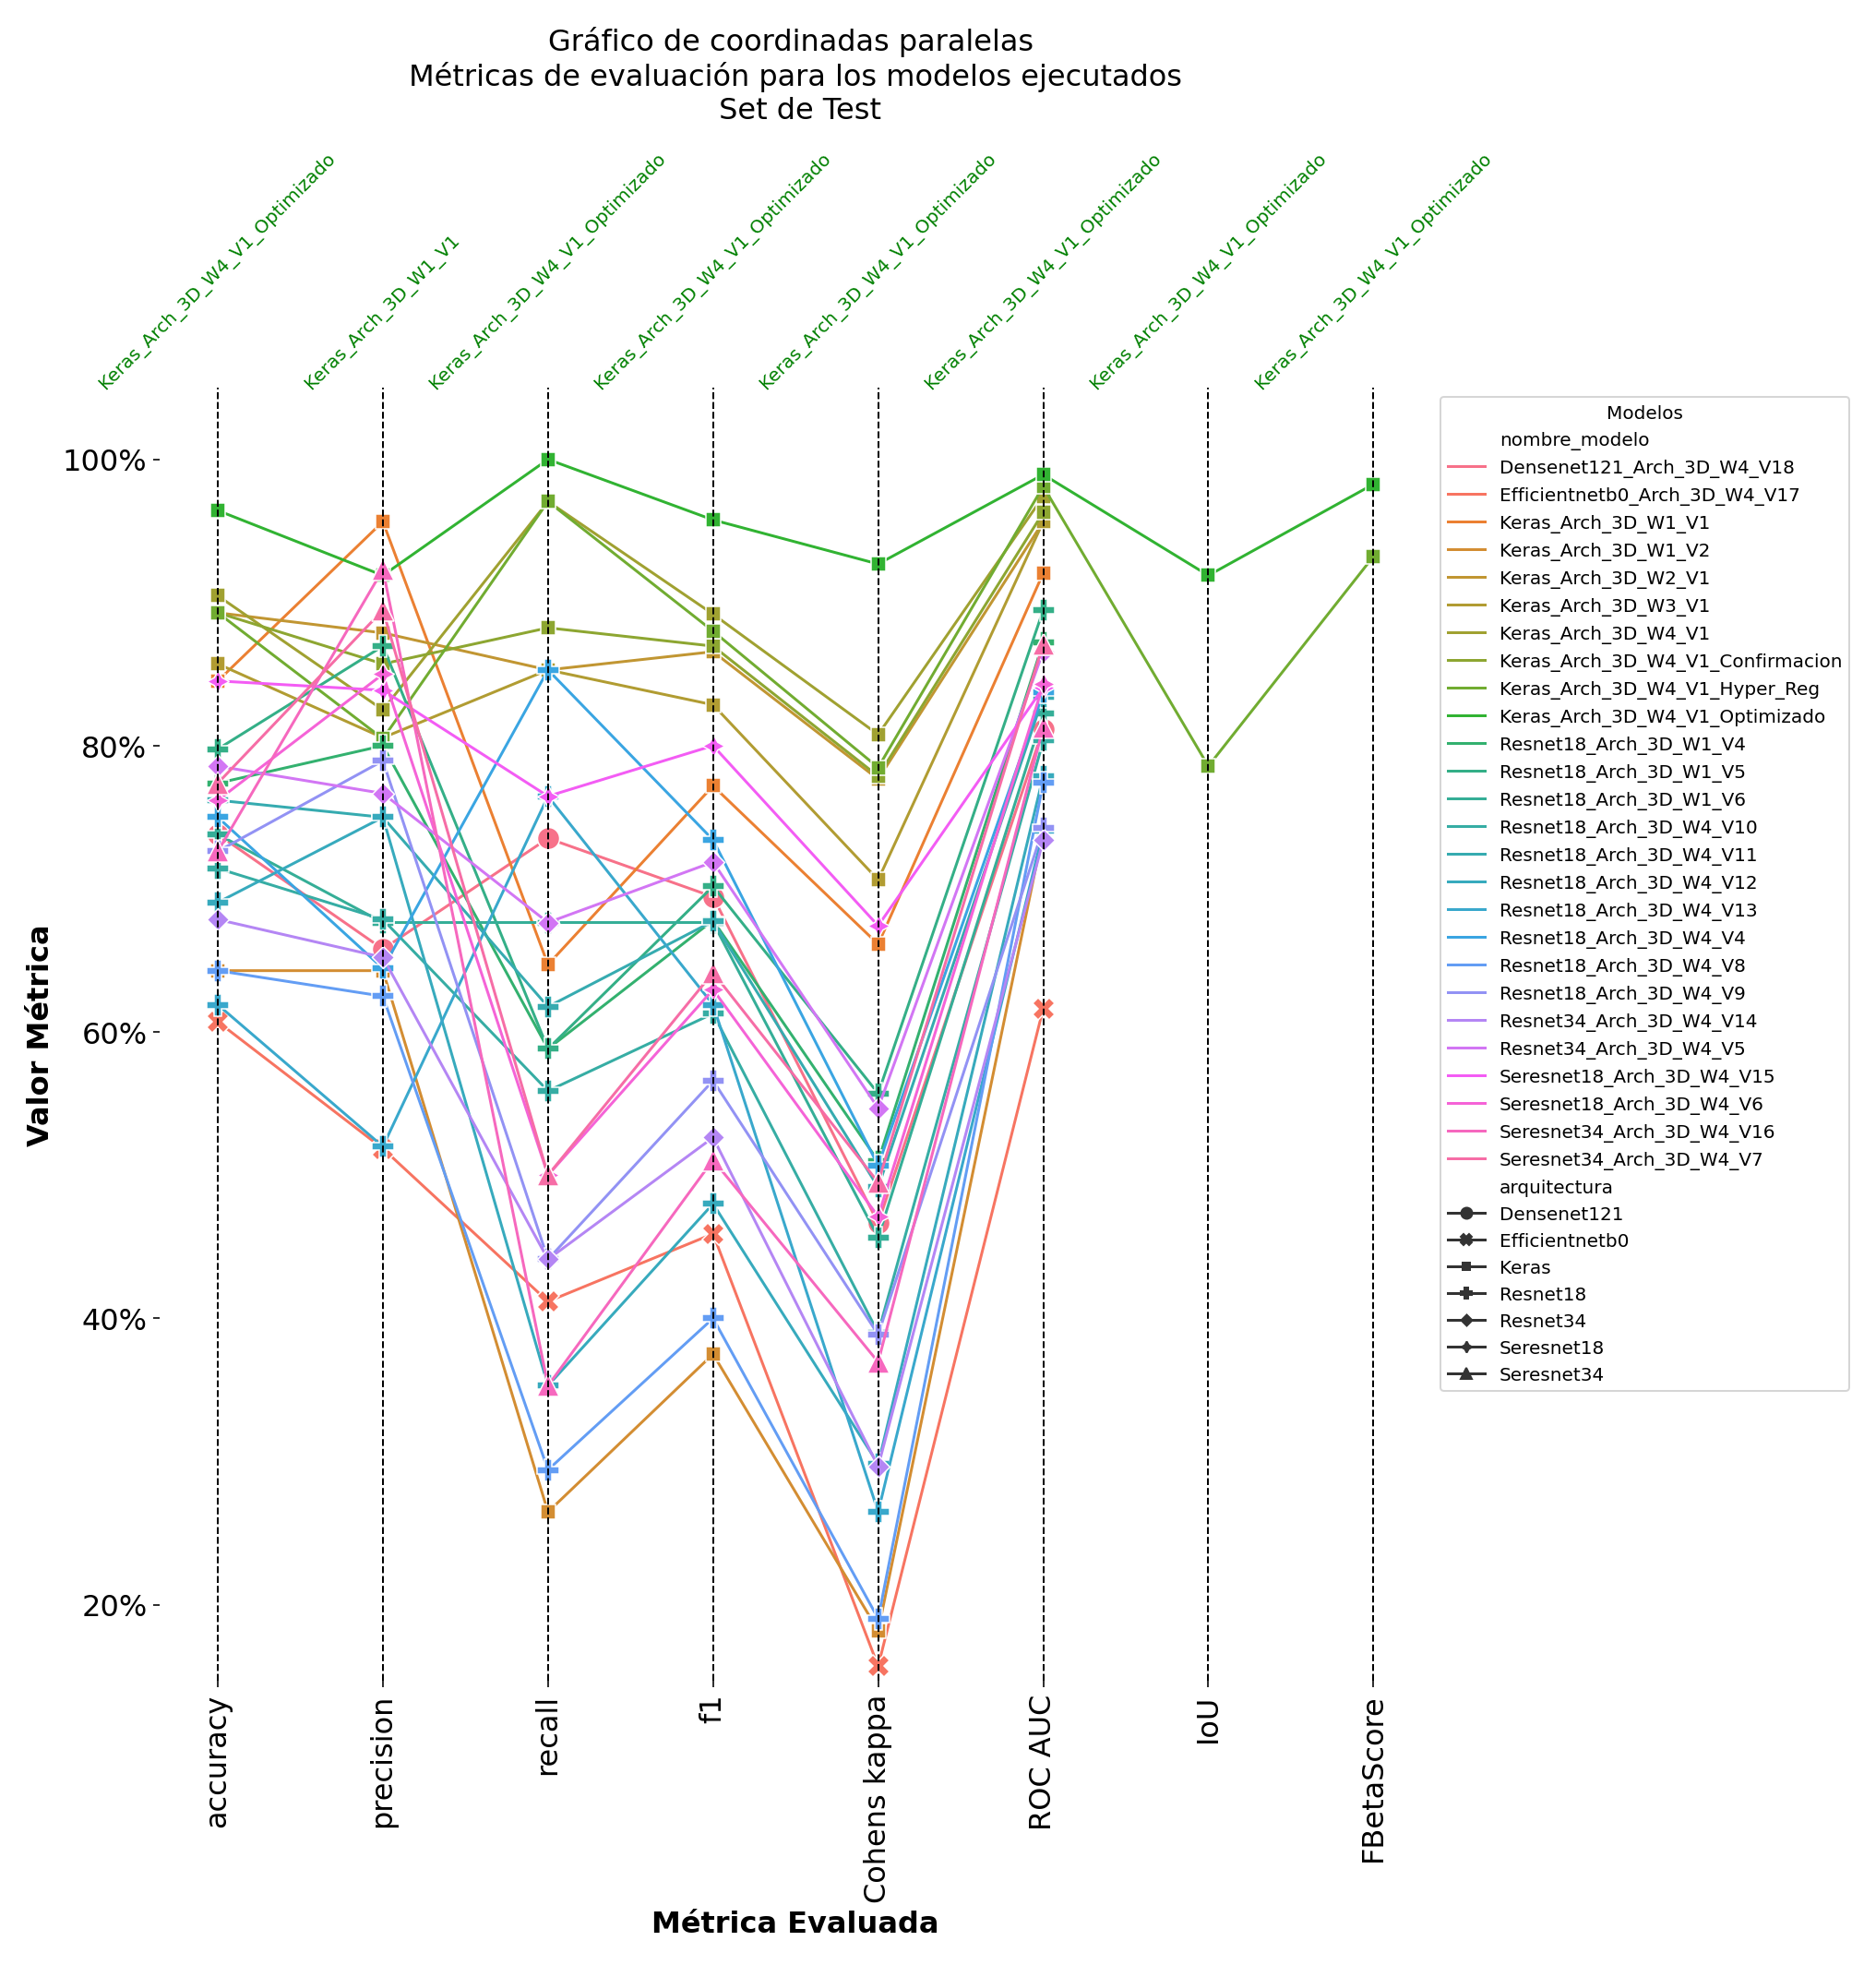
\includegraphics[scale=0.5]{G:/Mi unidad/Maestria/Tesis/Bayesian_NN/Modelos_Colab/Resultados_3D/metricas/todos_deterministas_Test.png}
	\caption{Contaste de métricas evaluadas en todos los modelos deterministas - Set de Test}
	\label{fig:deterministas_test_todos}
	\end{figure}

	\paragraph{Redes Bayesianas}

	El siguiente paso de exploración profundizó en el entrenamiento de redes neuronales bayesianas, comenzando con modificaciones menores en la arquitectura del modelo determinista optimizado. La principal alteración implicó reemplazar la última capa densa del modelo determinista con sus contrapartes bayesianas, (fragmentos de código Python en \ref{codigo_bayesiana_1})

	Estos cambios introducen estocasticidad en la salida del modelo, permitiéndole capturar la incertidumbre inherente a los datos y las predicciones. Al utilizar capas bayesianas, el modelo gana la capacidad de expresar incertidumbre en sus predicciones, ofreciendo así resultados más informativos en comparación con sus homólogos deterministas. Específicamente, las opciones 1A y 1B utilizan capas de Bernoulli independientes para modelar la distribución de salida binaria, mientras que las opciones 2A y 2B emplean capas \href{https://github.com/janosh/tf-mnf}{MNFDense} junto con capas de Bernoulli independientes para incorporar un flujo de normalización multiplicativo. Estas variaciones permiten diferentes enfoques para la cuantificación de la incertidumbre y la representación del modelo, lo que proporciona flexibilidad para modelar relaciones complejas dentro de los datos.

	Si bien las exploraciones iniciales no implicaron cálculos de las métricas para los conjuntos de datos, se llevó a cabo un análisis de la evolución del modelo época por época, centrándose en la precisión y la función de pérdida \ref{metricas_bayesiana_1}. Las observaciones revelaron que las redes neuronales bayesianas iniciales no lograron igualar el rendimiento del modelo determinista optimizado. 
	
	Además de las variaciones mencionadas anteriormente en la última capa, la experimentación adicional implicó ajustes a los parámetros de entrenamiento, específicamente aumentando el número de épocas y alterando la tasa de aprendizaje. Finalmente, se exploraron capas alternativas para evaluar su impacto en el rendimiento del modelo. Estos incluyeron la integración de las siguientes capas:
	
	\begin{itemize}
		\item Dense Flipout: Esta capa introduce estocasticidad aplicando la técnica "flipout" durante el entrenamiento, que perturba los pesos de la red. Al incorporar incertidumbre a través de perturbaciones de peso, Dense Flipout permite que el modelo capture y represente la incertidumbre aleatoria inherente a los datos.
		
		\item Reparametrización local densa: en esta capa se emplea el truco de reparametrización local (LRT), cuyo objetivo es aproximar la distribución de salida de la capa reparametrizando los pesos localmente. La reparametrización local densa mejora la capacidad del modelo para capturar y propagar la incertidumbre a través de la red.
		
		\item Reparametrización densa: similar a la reparametrización local densa, esta capa utiliza el truco de reparametrización para incorporar estocasticidad al modelo. Al repararmetrizar los pesos de la capa, facilitando la propagación de la incertidumbre a través de la red, permitiendo así un modelado más robusto y expresivo de distribuciones de datos complejas.
	\end{itemize}
	
	Tras la exploración de las variaciones en la última capa, el paso siguiente implicó reemplazar las capas convolucionales deterministas con sus contrapartes bayesianas en tres escenarios distintos:
	
	\begin{itemize}
		\item Enfoque 1: Capas convolucionales MNF 3D: en este enfoque, las capas convolucionales deterministas se sustituyeron por capas convolucionales bayesianas de flujos de normalización multiplicativa (MNF) 3D, aprovechando los resultados de la investigación en \cite{mnf}. Las capas MNF ofrecen un marco flexible para capturar distribuciones complejas de pesos, lo que permite representaciones más expresivas y conscientes de la incertidumbre dentro del modelo.
		
		\item Enfoque 2: Capas convolucionales Convolution3DFlipout: este enfoque implicó reemplazar las capas convolucionales deterministas con capas convolucionales Flipout. Las capas Flipout introducen estocasticidad en las operaciones convolucionales mediante la aplicación de la técnica "flipout", que perturba los pesos de los filtros convolucionales durante el entrenamiento.
		
		\item Enfoque 3: Capas convolucionales Convolution3DReparameterization: en este enfoque, las capas convolucionales deterministas se reemplazaron con capas convolucionales de reparametrización. Las capas de Reparametrización Convolution3D, aprovechan la técnica de Reparametrización para el muestreo de pesos. % La reparametrización reexpresa las variables aleatorias (pesos) en términos de transformaciones deterministas de distribuciones conocidas, lo que permite una optimización basada en gradientes y una estimación eficiente de la distribución posterior sobre los pesos.
		
	\end{itemize}

	Además de los enfoques de capas convolucionales bayesianas mencionados anteriormente, otra alternativa explorada fue la implementación de una red neuronal Monte Carlo Dropout. En este enfoque, se mantuvo la arquitectura del modelo optimizado determinista, con modificaciones realizadas en la capa dropout descritas en \ref{Monte_Carlo_Dropout}

	En la capa dropout modificada, la inclusión de ''training=True'' desempeña un papel importante a la hora de especificar el comportamiento de la misma durante la fase de entrenamiento de la red neuronal. Este argumento indica a la capa dropout que debe aplicar la regularización de abandono estableciendo aleatoriamente una fracción de unidades de entrada en cero durante cada iteración de entrenamiento. Al activar el abandono durante el entrenamiento, el modelo aprende a adaptarse y generalizar de manera más efectiva, ya que está expuesto a diferentes patrones de abandono en cada época de entrenamiento. Esta estocasticidad introducida por la regularización de abandonos ayuda a prevenir el sobreajuste y mejora la capacidad del modelo para generalizar a datos nuevos.
		
	Después de evaluar varias alternativas de arquitectura bayesiana, los hallazgos de la Fig.(~\ref{fig:bayesianas_test}) indican que la red neuronal bayesiana que comprende capas convolucionales de flujo de normalización multiplicativos (MNF) y una capa de salida densa de MNF demuestra un rendimiento superior en las métricas evaluadas en el conjunto de datos de testeo. Esta arquitectura bayesiana logra un rendimiento comparable al de la red neuronal determinista seleccionada, demostrando su eficacia a la hora de clasificar la neumonía por COVID-19 en tomografías computarizadas en 3D. 
	
	Al aprovechar las capas convolucionales de MNF y la capa de salida densa de MNF, esta red neuronal bayesiana captura de manera efectiva la incertidumbre subyacente inherente a los datos, mejorando así sus capacidades predictivas. Estos resultados subrayan la importancia de los enfoques bayesianos en las tareas de imágenes médicas, particularmente para proporcionar predicciones sólidas y confiables al tiempo que cuantifican la incertidumbre. 
	
	El siguiente gráfico de coordenadas paralelas resume el rendimiento de todos los modelos bayesianos evaluados y ofrece información valiosa sobre su rendimiento comparativo y destaca la eficacia de la red neuronal bayesiana basada en MNF (Modelo: Keras\_Arch\_3D\_W4\_V1\_Uncertainty\_V4\_3C) \footnote{Más detalle sobre los nombres de los modelos en \ref{anexo_tabla_modelos}}.
	
	\begin{figure}[H]
	\centering
	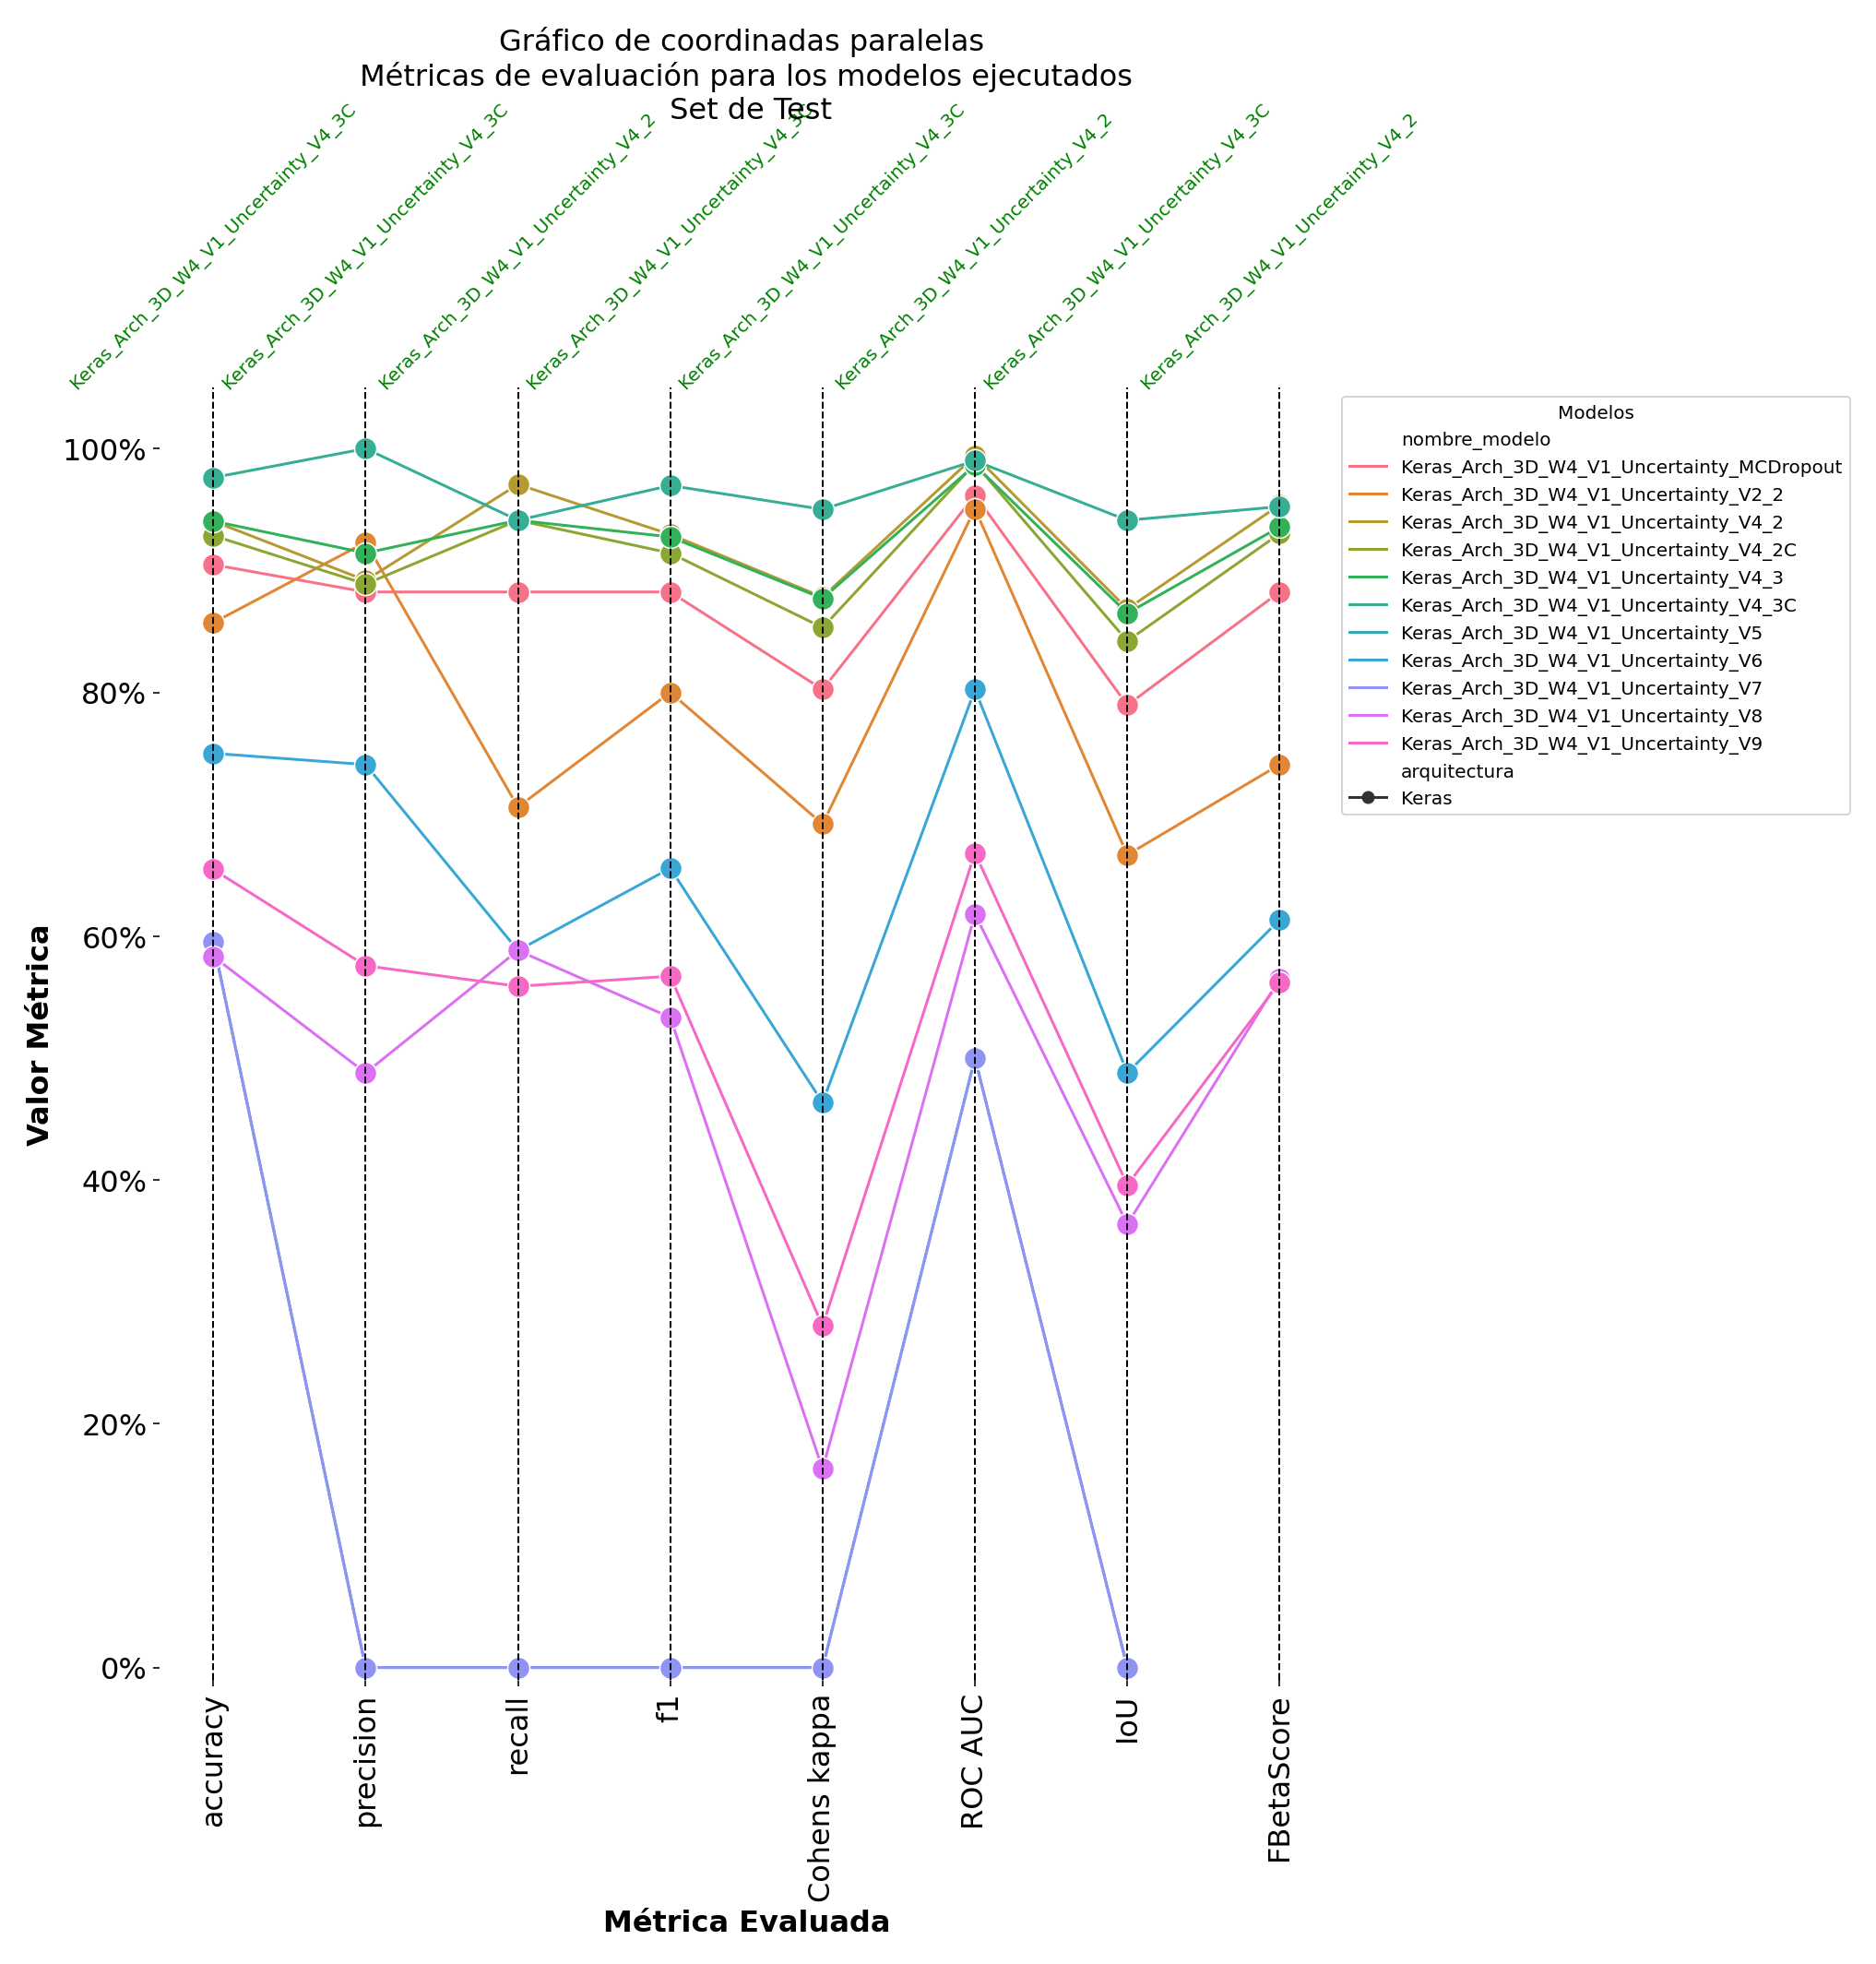
\includegraphics[scale=0.5]{G:/Mi unidad/Maestria/Tesis/Bayesian_NN/Modelos_Colab/Resultados_3D/metricas/bayesian_3D_test.png}
	\caption{Contaste de métricas evaluadas en los modelos Bayesianos - Set de Test}
	\label{fig:bayesianas_test}
	\end{figure}
	

	\subsubsection{Calibración:} \label{r_calibracion_3d}

	El análisis de calibración de los modelos implicó la visualización de diagramas de confiabilidad y el cálculo del Error de Calibración Esperado (ECE). Estos análisis se realizaron para una variedad de modelos\footnote{La descripción de cada modelo la pueden encontrar en \ref{anexo_tabla_modelos}} con el fin de evaluar su desempeño de calibración e identificar configuraciones óptimas.
	
	Los modelos considerados para el análisis de calibración incluyeron:

	\begin{itemize}
		\item Keras\_Arch\_3D\_W4\_V1\_Confirmacion 
		\item Keras\_Arch\_3D\_W4\_V1\_Optimizado
		\item Keras\_Arch\_3D\_W4\_V1\_Uncertainty\_V4\_2C
		\item Keras\_Arch\_3D\_W4\_V1\_Uncertainty\_V4\_3C
		\item Keras\_Arch\_3D\_W4\_V1\_Uncertainty\_V6
		\item Keras\_Arch\_3D\_W4\_V1\_Uncertainty\_MCDropout
	\end{itemize}	
	

	Además de evaluar diferentes modelos, se realizaron experimentos para evaluar el impacto de cambiar la capa probabilística de Bernoulli de los modelos bayesianos a una capa de activación \textsl{Sigmoid}.
	
	Los resultados del análisis de calibración revelaron varias ideas clave:
	
	\begin{itemize}
		\item Efecto de la capa de activación \textsl{Sigmoid}: la sustitución de la capa probabilística de Bernoulli por una capa de activación \textsl{Sigmoid} en las redes neuronales bayesianas no parece afectar significativamente la calidad de las predicciones de clase. Las comparaciones de gráficos de coordenadas paralelas entre modelos con y sin la capa de activación \textsl{Sigmoid} ilustraron un rendimiento consistente en la mayoría de las métricas de clasificación \ref{coordenadas_paralelas}.
		
		\item Punto de corte óptimo: Un hallazgo notable fue la identificación de un punto de corte óptimo (umbral) para las predicciones de clase 1. Si bien el umbral predeterminado se había establecido en 0.5 en experimentos anteriores, el análisis reveló un mejor rendimiento de las métricas cuando el umbral se ajustó a 0.4. Este ajuste resultó en una mayor precisión de clasificación y otras métricas relacionadas \ref{coordenadas_paralelas_umbral}.
		
		\item Confiabilidad y métricas ECE: entre los modelos evaluados, dos emergieron como los de mejor desempeño en términos de confiabilidad y métricas ECE. Para los modelos deterministas, Keras\_Arch\_3D\_W4\_V1\_Optimizado (Fig.(~\ref{fig:conf_determinsita})) demostró consistentemente una sólida calibración en diferentes configuraciones de umbral. Su histograma de confiabilidad exhibió líneas verticales estrechamente alineadas y un alto nivel de confianza, indicativo de predicciones confiables. De manera similar, para los modelos bayesianos, Keras\_Arch\_3D\_W4\_V1\_Uncertainty\_V4\_3C (Fig.(\ref{fig:conf_bayesiana})) con la capa \textsl{Sigmoid} y un umbral de 0.4 mostró excelentes características de calibración, con líneas verticales muy agrupadas y una desviación mínima de la diagonal \ref{resultados_diagrama_conf}.
		
	\begin{figure}[H]
	\centering
	\begin{subfigure}[H]{0.45\textwidth} %
		\centering
		\includegraphics[scale=0.5]{G:/Mi unidad/Maestria/Tesis/Bayesian_NN/Modelos_Colab/Resultados_3D/calibraciones/imagenes/test_datasets/Keras_Arch_3D_W4_V1_Optimizado_Corte50_test.png}
		\caption{Red Neuronal Determinista}
		\label{fig:conf_determinsita}
	\end{subfigure}
	\hfill
	\begin{subfigure}[H]{0.45\textwidth} % \textwidth
		\centering
		\includegraphics[scale=0.5]{G:/Mi unidad/Maestria/Tesis/Bayesian_NN/Modelos_Colab/Resultados_3D/calibraciones/imagenes/test_datasets/Keras_Arch_3D_W4_V1_Uncertainty_V4_3C_Sigmoid_Corte40_test.png}
		\caption{Red Neuronal Bayesiana}
		\label{fig:conf_bayesiana}
	\end{subfigure}
	\caption{Diagrama de Confiabilidad e Histograma - Set de Test}
	\label{fig:conf_mejores}
	\end{figure}
		
	\end{itemize}		
	
	Los diagramas de confiabilidad en la Fig.(~\ref{fig:conf_mejores}) de estos modelos de alto rendimiento reforzaron aún más la calidad de su calibración, y los histogramas representan predicciones bien calibradas y discrepancias mínimas entre confianza y precisión. Estos hallazgos subrayan la importancia del análisis de calibración para evaluar la confiabilidad de los modelos de aprendizaje automático.

	\subsubsection{Incertidumbre:} \label{r_incertidumbre_3d}
	
	El análisis de incertidumbre de los modelos implicó el análisis de intervalos de predicción derivados de ejercicios de simulación realizados en imágenes de TC seleccionadas mencionado en la sección \ref{metodologia_3D}. Estas imágenes abarcaban una variedad de clases y se utilizaron para evaluar el rendimiento predictivo y las capacidades de estimación de incertidumbre de los modelos deterministas y bayesianos.
	
	De forma aleatoria, se seleccionaron seis imágenes para el análisis, comprendidas por cuatro imágenes que representan clases con distintos grados de afectación de neumonía (CT-1 y CT-4) desconocidas por el modelo y dos imágenes del conjunto de datos de testeo etiquetadas como no afectadas por neumonía (CT-0).
	
	El análisis se centró en contrastar las predicciones y la incertidumbre (en el escenario bayesiano) de los dos mejores modelos elegidos en etapas anteriores: el modelo determinista (Keras\_Arch\_3D\_W4\_V1\_Optimizado) y el modelo bayesiano (Keras\_Arch\_3D\_W4\_V1\_Uncertainty\_V4\_3C +  Sigmoid). Estos modelos fueron seleccionados en función de su desempeño y representatividad en el contexto del estudio.
	
	\paragraph{Análisis de imágenes individuales:}
	
	\begin{itemize}
	\item Imágenes de clase CT-1:
	
	\begin{itemize}
	\item Imagen 1 (Fig.(~\ref{fig:layout})): Tanto el modelo determinista como el bayesiano identificaron correctamente deficiencias en la tomografía, clasificándola como clase 1 (presencia de afectación). Sin embargo, el modelo bayesiano destacó al ofrecer intervalos de predicción estrechos, indicando alta confianza en sus predicciones. Esta capacidad de cuantificar la incertidumbre de manera precisa es esencial en aplicaciones médicas, ya que permite una toma de decisiones más informada y precisa. Estos resultados resaltan la utilidad de los modelos bayesianos en el diagnóstico médico.
	Los intervalos de confianza para cada clase por el modelo bayesiano son:
	\begin{itemize}
	\item Clase 0: [0.0001179 - 0.08210155] 
	\item Clase 1: [0.91789845 - 0.9998821]
	\end{itemize} 

\begin{figure}[H]
	\centering
	\begin{subfigure}[b]{0.6\textwidth}
		\centering
		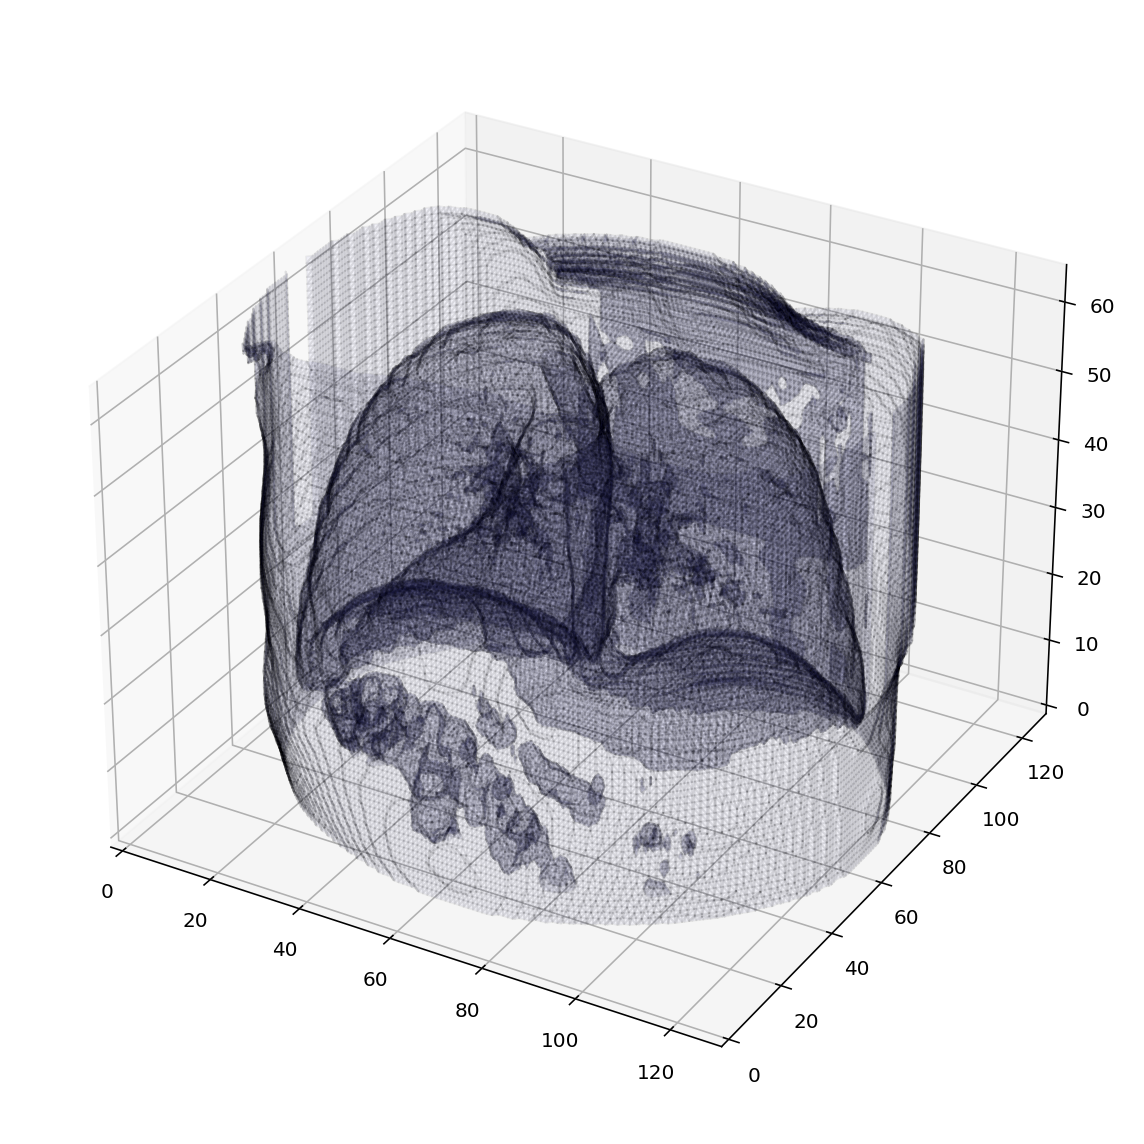
\includegraphics[width=0.5\textwidth]{G:/Mi unidad/Maestria/Tesis/Bayesian_NN/Modelos_Colab/Resultados_3D/metricas/1_ct_1.png} % Adjust the width as needed
		\caption{Representación 3D Tomografía}
		\label{fig:1_ct1_1}
	\end{subfigure}
	
	\medskip
	
	\begin{subfigure}[b]{0.45\textwidth}
		\centering
		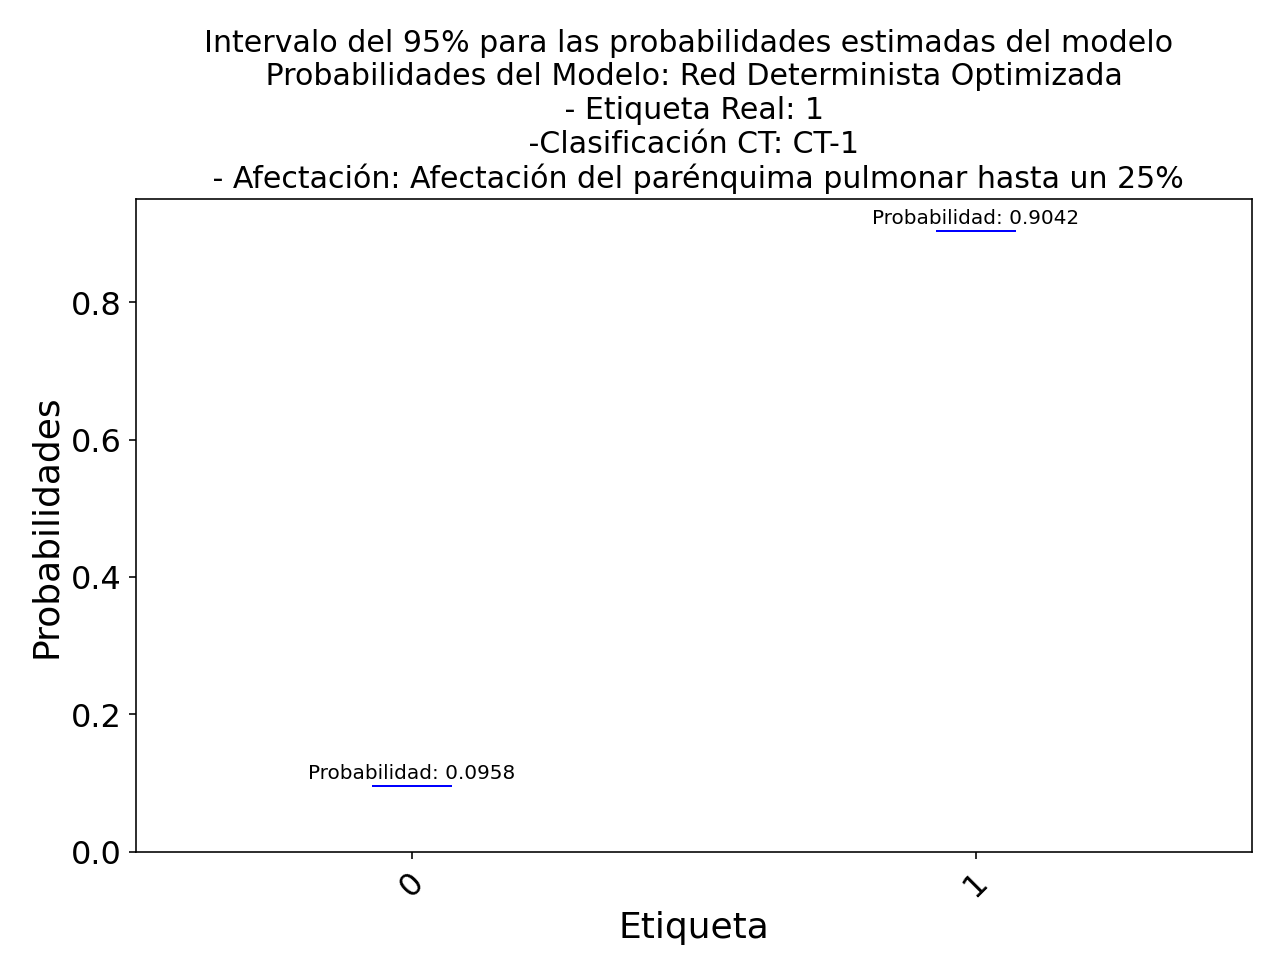
\includegraphics[scale=0.25]{G:/Mi unidad/Maestria/Tesis/Bayesian_NN/Modelos_Colab/Resultados_3D/metricas/1_ct_1_determinista.png}
		\caption{Red Neuronal Determinista}
		\label{fig:1_ct1_2}
	\end{subfigure}
	\hfill
	\begin{subfigure}[b]{0.45\textwidth}
		\centering
		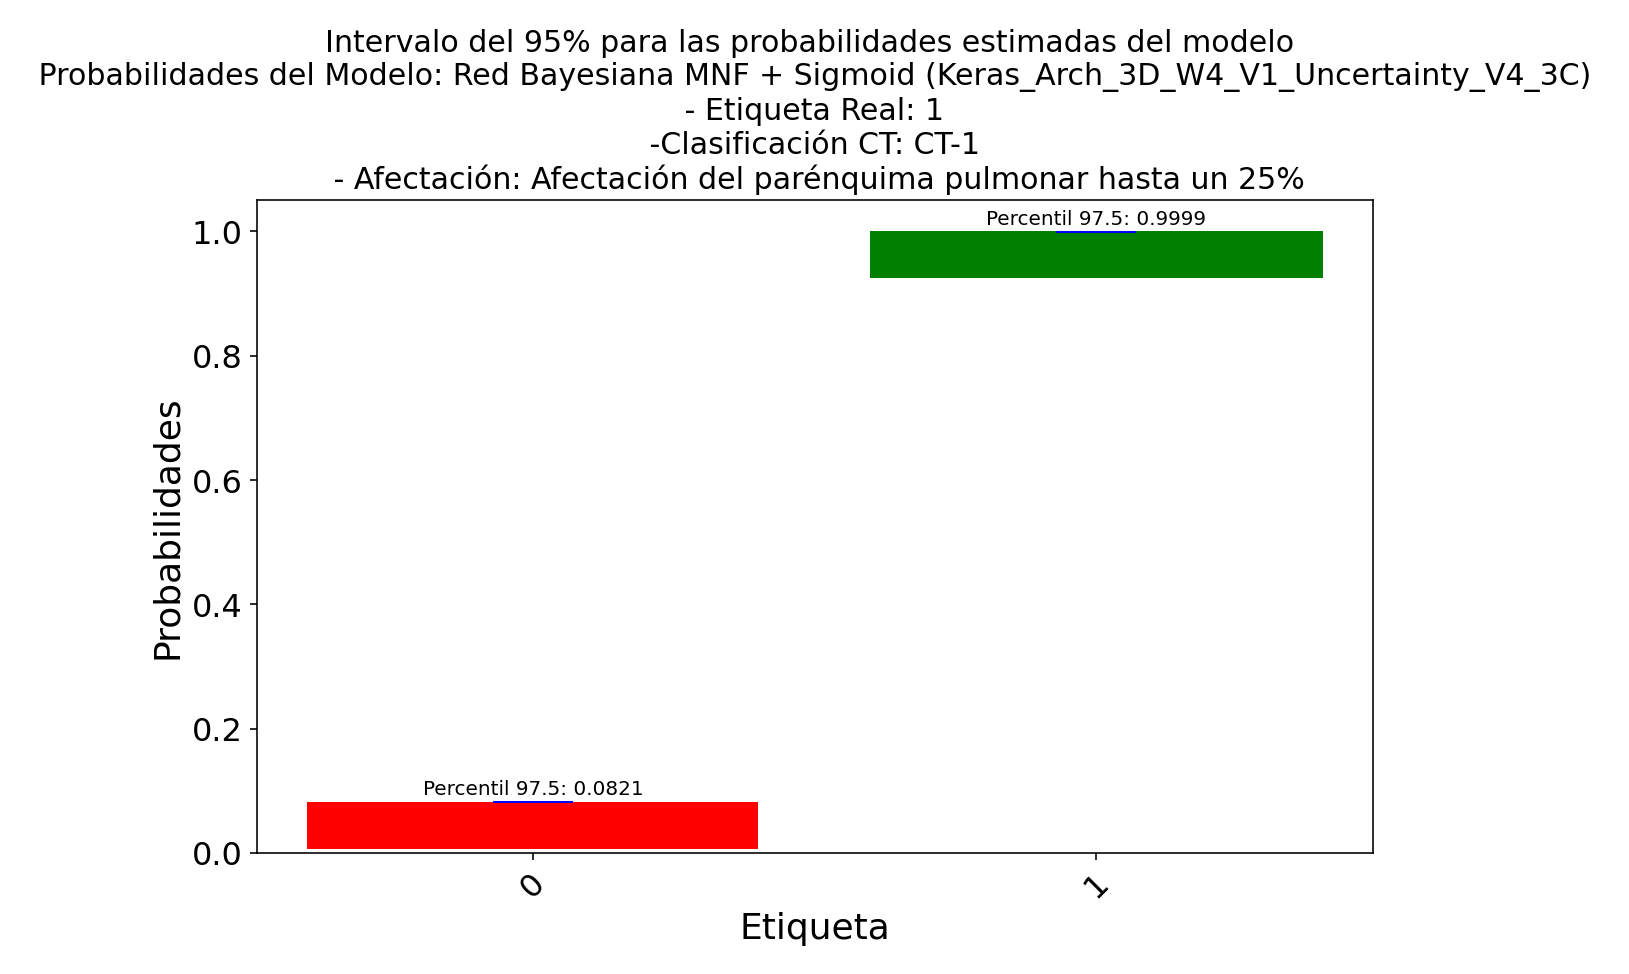
\includegraphics[scale=0.25]{G:/Mi unidad/Maestria/Tesis/Bayesian_NN/Modelos_Colab/Resultados_3D/metricas/1_ct_1_mnf_sigmoid.png}
		\caption{Red Neuronal Bayesiana}
		\label{fig:1_ct1_3}
	\end{subfigure}
	
	\caption{Análisis Incertidumbre - Imagen 1: CT-1}
	\label{fig:layout}
\end{figure}
	
	\item Imagen 2 (Fig.(~\ref{fig:layout_2})): Ambos modelos concuerdan en que la tomografía analizada no presenta ninguna afectación (es decir, clase 0), no obstante esta afirmación no es precisa, ya que la imagen pertenece a una clase con un compromiso del parénquima pulmonar del 25\%. A pesar de este error en la predicción, la red bayesiana ofrece intervalos de confianza notablemente amplios, lo que sugiere la presencia de incertidumbre. Este resultado resalta la importancia de considerar la incertidumbre en las predicciones, incluso cuando estas son incorrectas, proporcionando así una evaluación más cautelosa del diagnóstico médico.
	Los intervalos de confianza para cada clase por el modelo bayesiano son:
	
	\begin{itemize}
	\item Clase 0: [0.85678702 - 0.99927345 ]
	\item Clase 1: [0.00072655 - 0.14321298]
	\end{itemize}

\begin{figure}[H]
	\centering
	\begin{subfigure}[b]{0.6\textwidth}
		\centering
		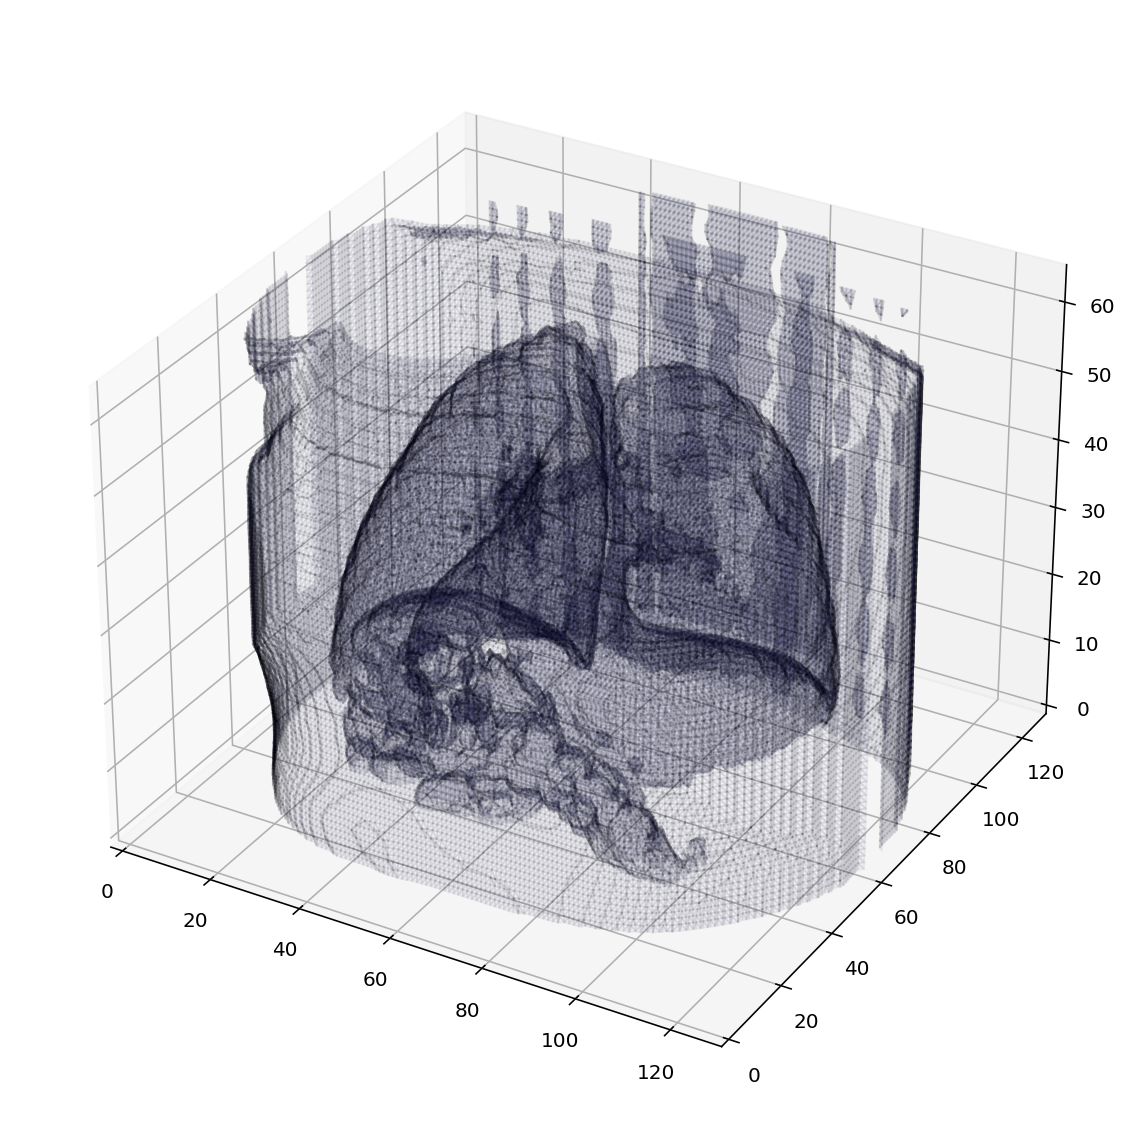
\includegraphics[width=0.5\textwidth]{G:/Mi unidad/Maestria/Tesis/Bayesian_NN/Modelos_Colab/Resultados_3D/metricas/2_ct_1.png} % Adjust the width as needed
		\caption{Representación 3D Tomografía}
		\label{fig:2_ct1_1}
	\end{subfigure}
	
	\medskip
	
	\begin{subfigure}[b]{0.45\textwidth}
		\centering
		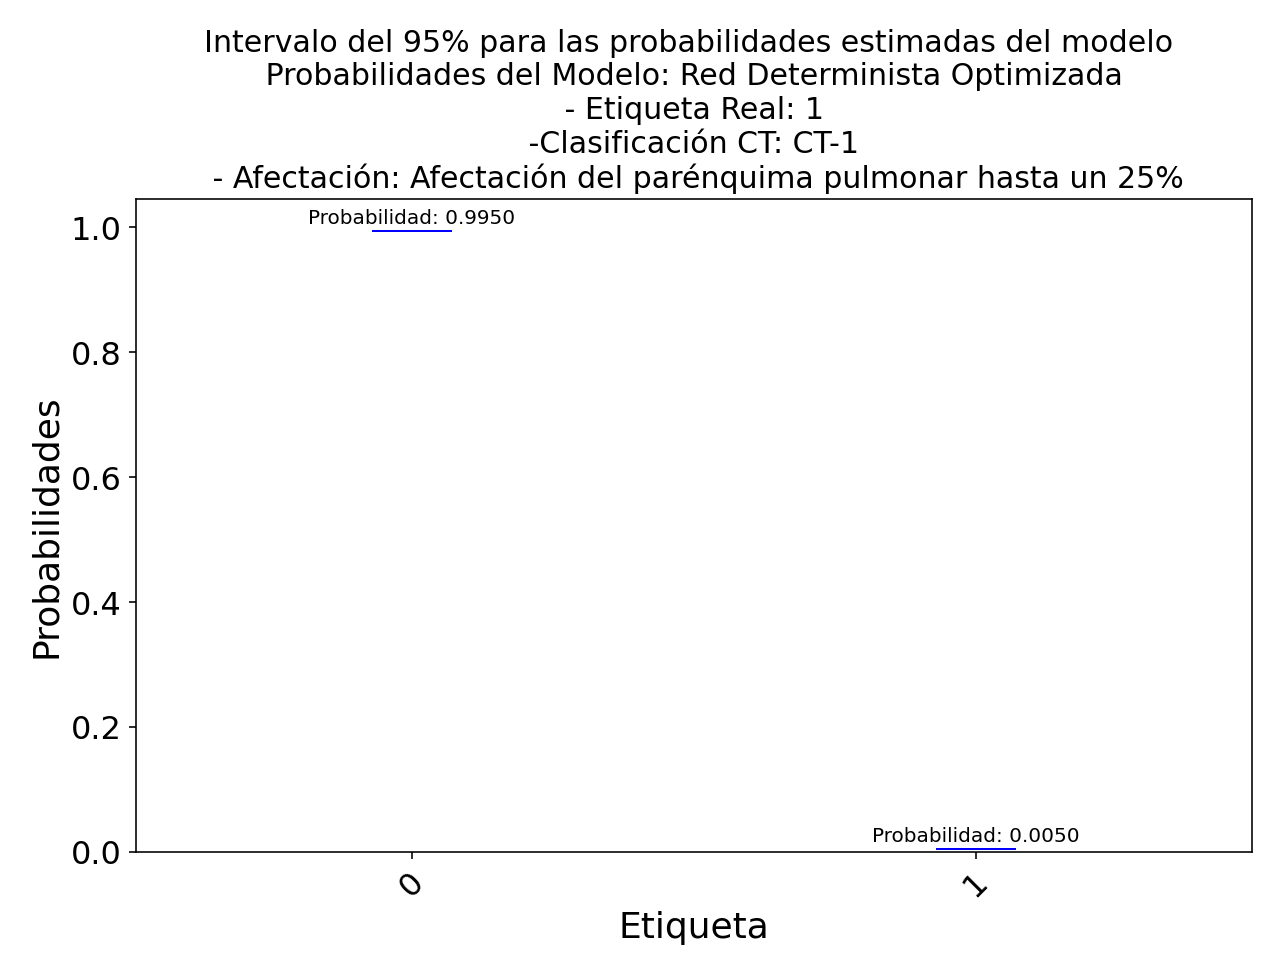
\includegraphics[scale=0.25]{G:/Mi unidad/Maestria/Tesis/Bayesian_NN/Modelos_Colab/Resultados_3D/metricas/2_ct_1_determinista.png}
		\caption{Red Neuronal Determinista}
		\label{fig:2_ct1_2}
	\end{subfigure}
	\hfill
	\begin{subfigure}[b]{0.45\textwidth}
		\centering
		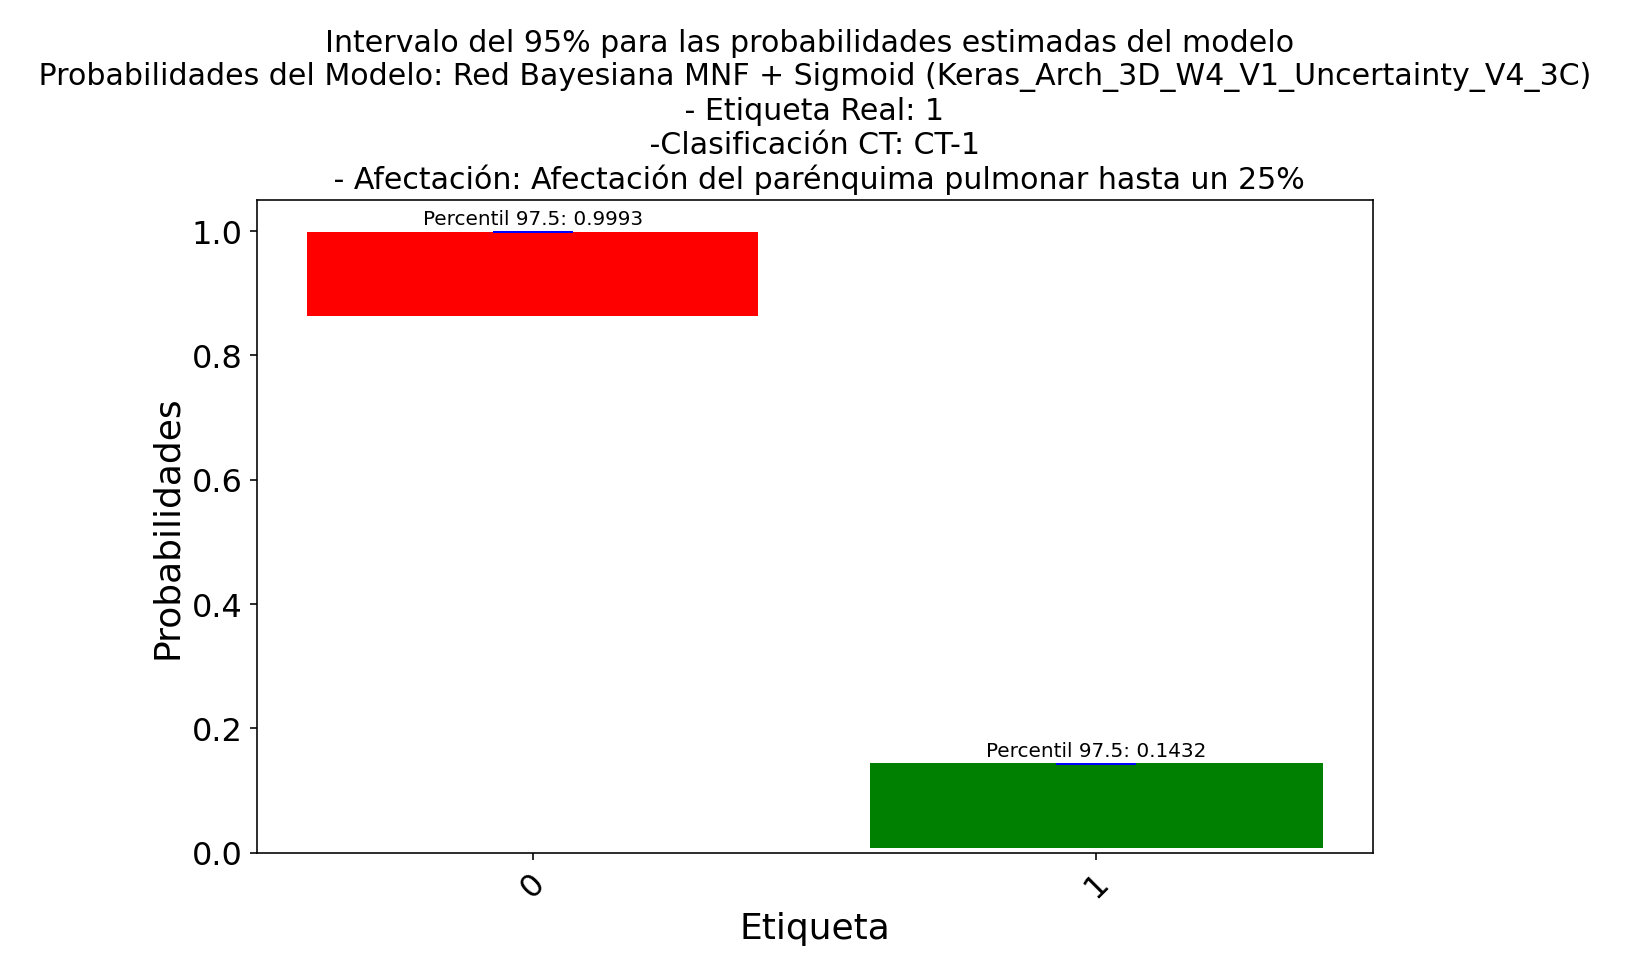
\includegraphics[scale=0.25]{G:/Mi unidad/Maestria/Tesis/Bayesian_NN/Modelos_Colab/Resultados_3D/metricas/2_ct_1_mnf_sigmoid.png}
		\caption{Red Neuronal Bayesiana}
		\label{fig:2_ct1_3}
	\end{subfigure}
	
	\caption{Análisis Incertidumbre - Imagen 2: CT-1}
	\label{fig:layout_2}
\end{figure}	
	
	\end{itemize}
	
	\item Imágenes de clase CT-4:
	
	\begin{itemize}
	\item Imagen 3 (Fig.(~\ref{fig:layout_3})): Ambos modelos identificaron correctamente alteraciones en la tomografía analizada, clasificándola como perteneciente a la clase 1. Sin embargo, los intervalos de predicción del modelo bayesiano tienen una amplitud bastante considerable, indicando una mayor incertidumbre en sus predicciones. Esta amplia incertidumbre podría ser considerada como una señal para generar alertas o solicitar una revisión adicional por parte de los profesionales médicos, con el fin de asegurar una evaluación más precisa y evitar posibles fallos diagnósticos. 
	Los intervalos de confianza para cada clase por el modelo bayesiano son:
	\begin{itemize}
	\item Clase 0: [0.00087272 - 0.36155368] 
	\item Clase 1: [0.63844632 - 0.99912728]
	\end{itemize} 

\begin{figure}[H]
	\centering
	\begin{subfigure}[b]{0.6\textwidth}
		\centering
		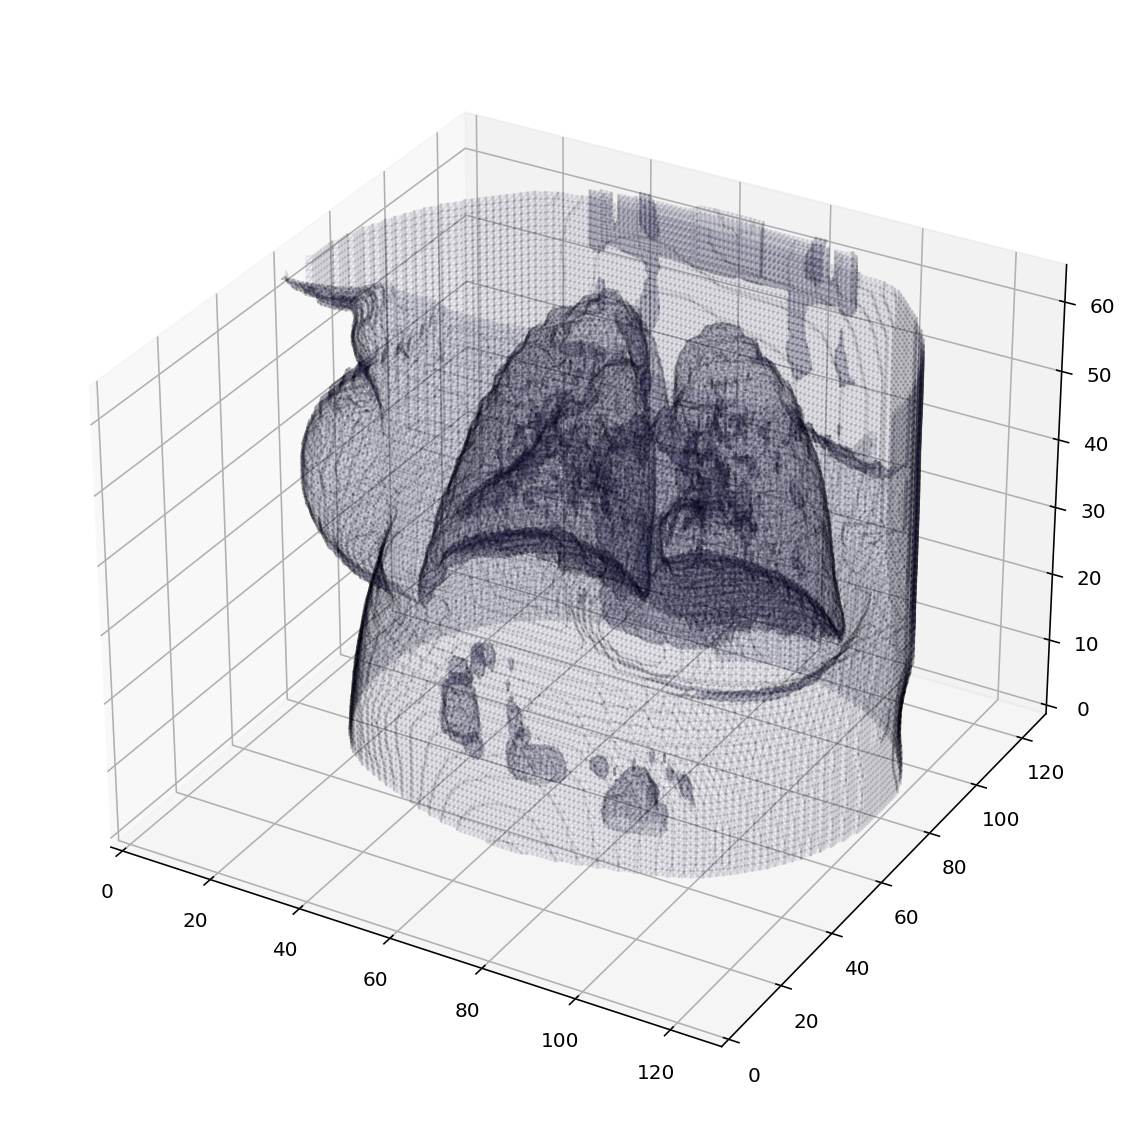
\includegraphics[width=0.5\textwidth]{G:/Mi unidad/Maestria/Tesis/Bayesian_NN/Modelos_Colab/Resultados_3D/metricas/3_ct_4.png} % Adjust the width as needed
		\caption{Representación 3D Tomografía}
		\label{fig:3_ct4_1}
	\end{subfigure}
	
	\medskip
	
	\begin{subfigure}[b]{0.45\textwidth}
		\centering
		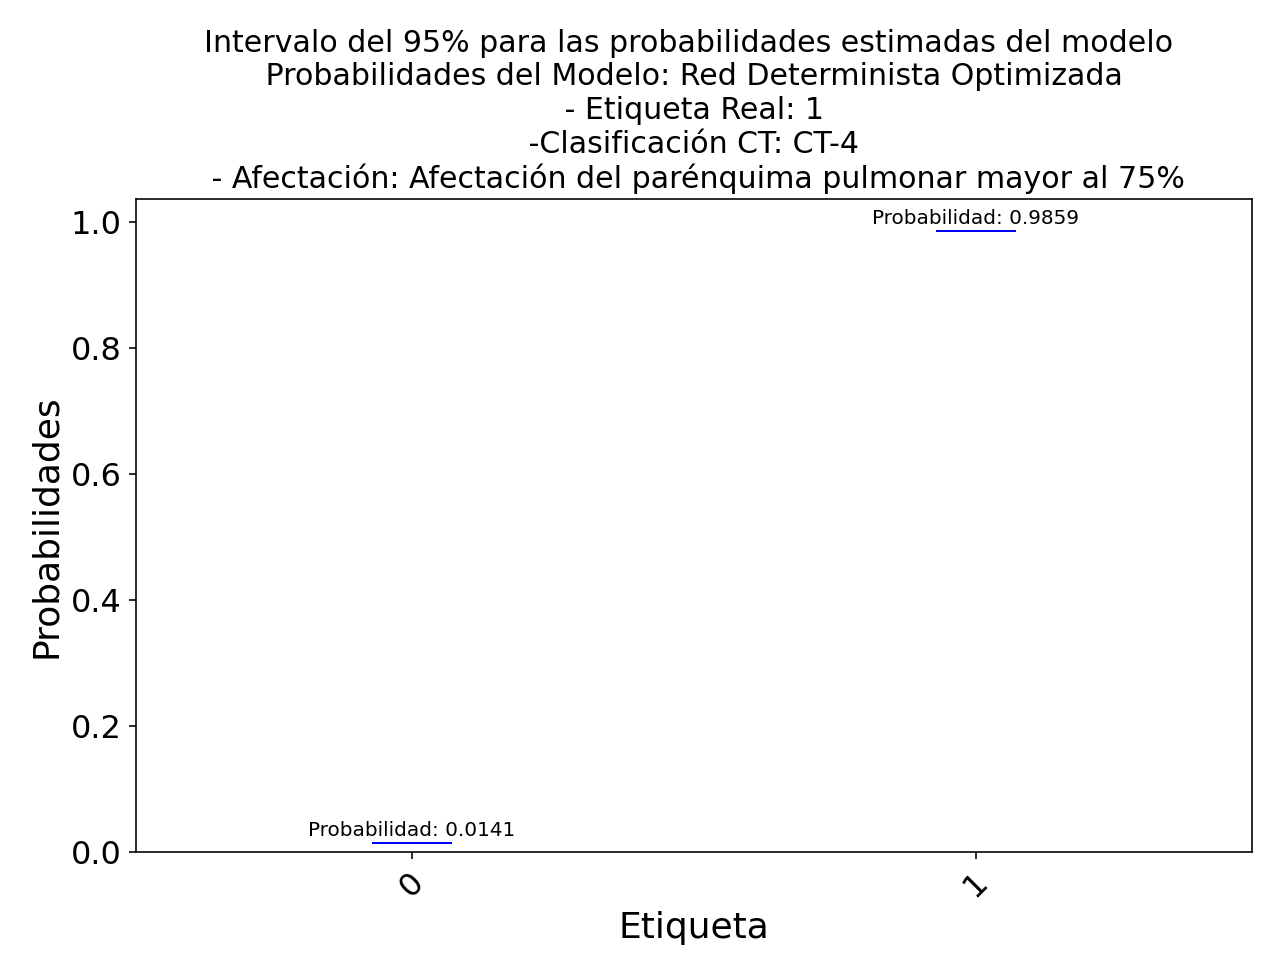
\includegraphics[scale=0.25]{G:/Mi unidad/Maestria/Tesis/Bayesian_NN/Modelos_Colab/Resultados_3D/metricas/3_ct_4_determinista.png}
		\caption{Red Neuronal Determinista}
		\label{fig:3_ct4_2}
	\end{subfigure}
	\hfill
	\begin{subfigure}[b]{0.45\textwidth}
		\centering
		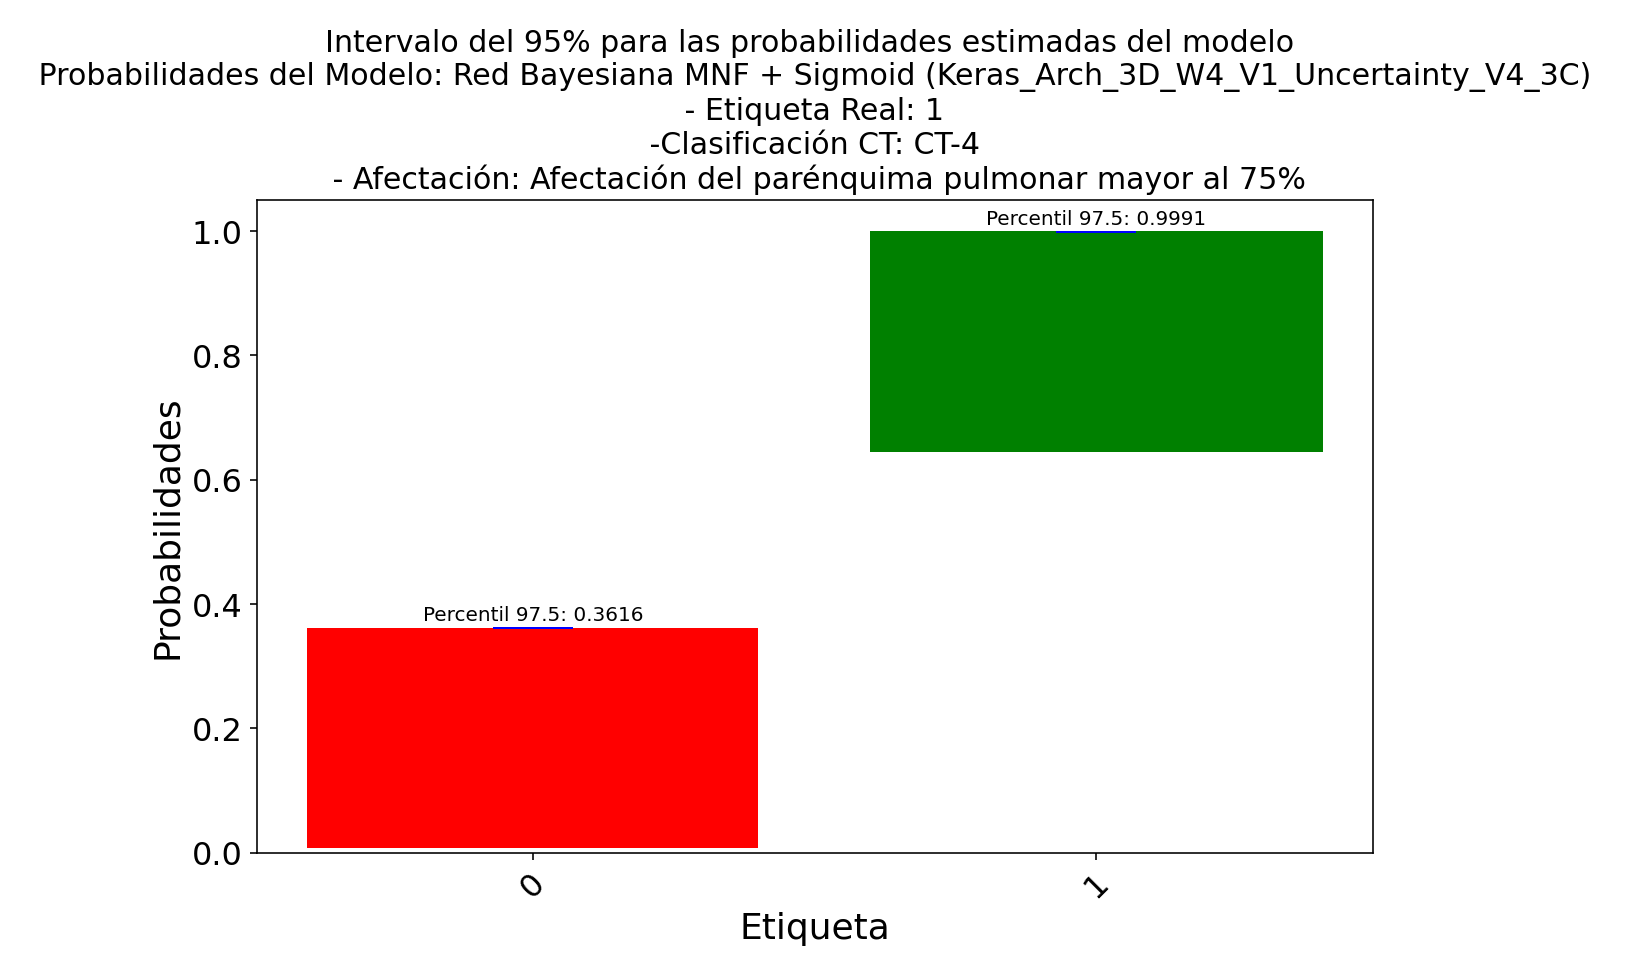
\includegraphics[scale=0.25]{G:/Mi unidad/Maestria/Tesis/Bayesian_NN/Modelos_Colab/Resultados_3D/metricas/3_ct_4_mnf_sigmoid.png}
		\caption{Red Neuronal Bayesiana}
		\label{fig:3_ct4_3}
	\end{subfigure}
	
	\caption{Análisis Incertidumbre - Imagen 3: CT-4}
	\label{fig:layout_3}
\end{figure}
	
	\item Imagen 4 (Fig.(~\ref{fig:layout_4})): De manera similar a la imagen de clase CT-4 anterior (Fig.(~\ref{fig:layout_3})), ambos modelos identificaron correctamente las deficiencias en la tomografía como clase 1. Sin embargo, resulta interesante observar que los intervalos de predicción del modelo bayesiano fueron notablemente estrechos, lo que sugiere una incertidumbre extremadamente baja en sus predicciones. Esta estrechez en los intervalos de predicción del modelo bayesiano apunta a una confiabilidad excepcional en sus resultados, remarcando su capacidad para realizar predicciones precisas y fiables incluso en situaciones complejas.
	Los intervalos de confianza para cada clase por el modelo bayesiano son:
	\begin{itemize}
	\item Clase 0: [0.0 - 0.00002203]
	\item Clase 1: [0.99997797 - 1.0]
	\end{itemize}

\begin{figure}[H]
	\centering
	\begin{subfigure}[b]{0.6\textwidth}
		\centering
		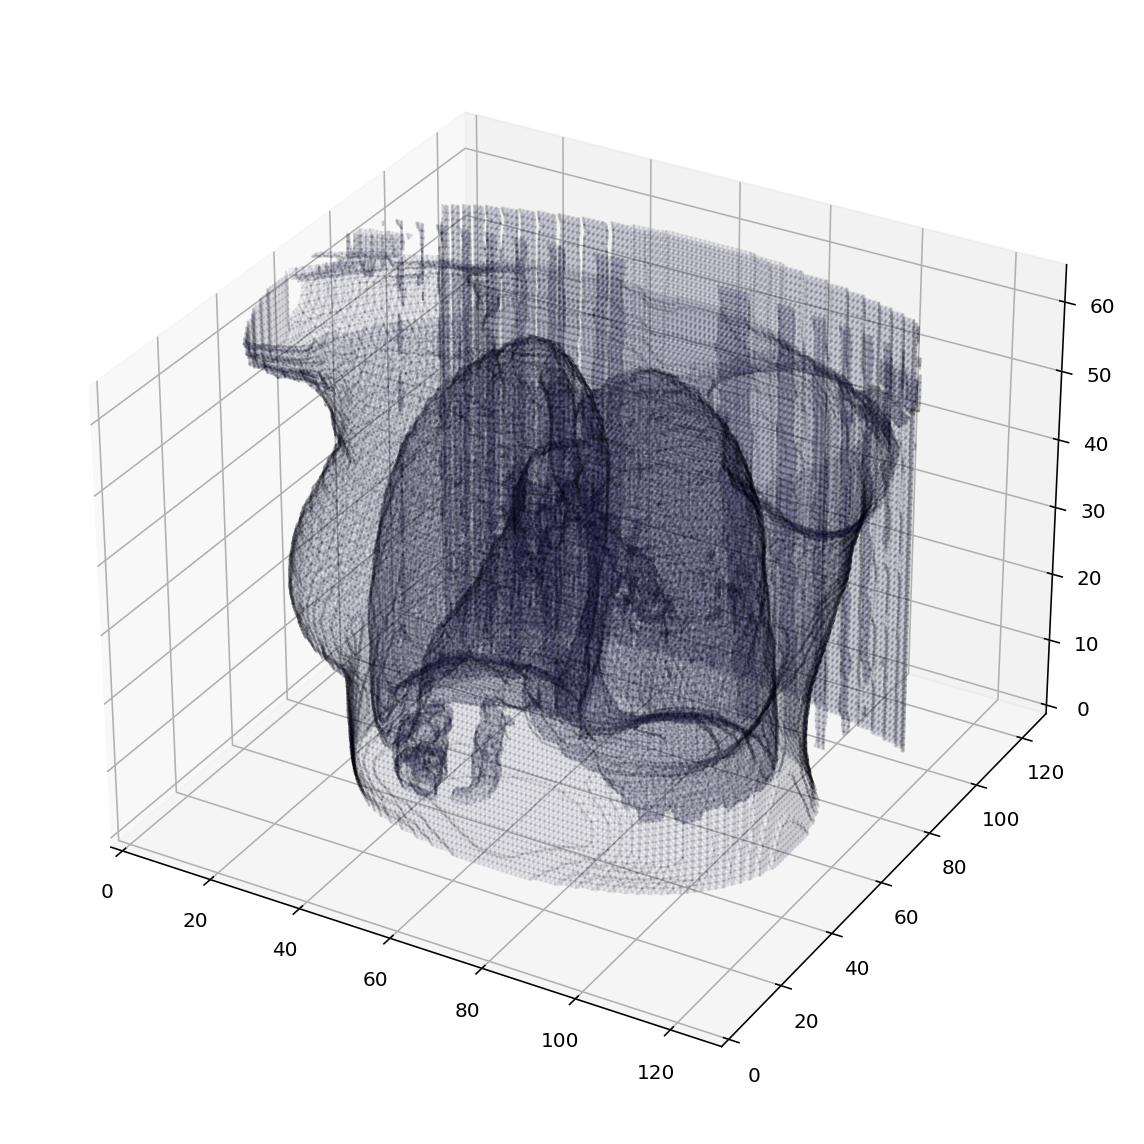
\includegraphics[width=0.5\textwidth]{G:/Mi unidad/Maestria/Tesis/Bayesian_NN/Modelos_Colab/Resultados_3D/metricas/4_ct_4.png} % Adjust the width as needed
		\caption{Representación 3D Tomografía}
		\label{fig:4_ct4_1}
	\end{subfigure}
	
	\medskip
	
	\begin{subfigure}[b]{0.45\textwidth}
		\centering
		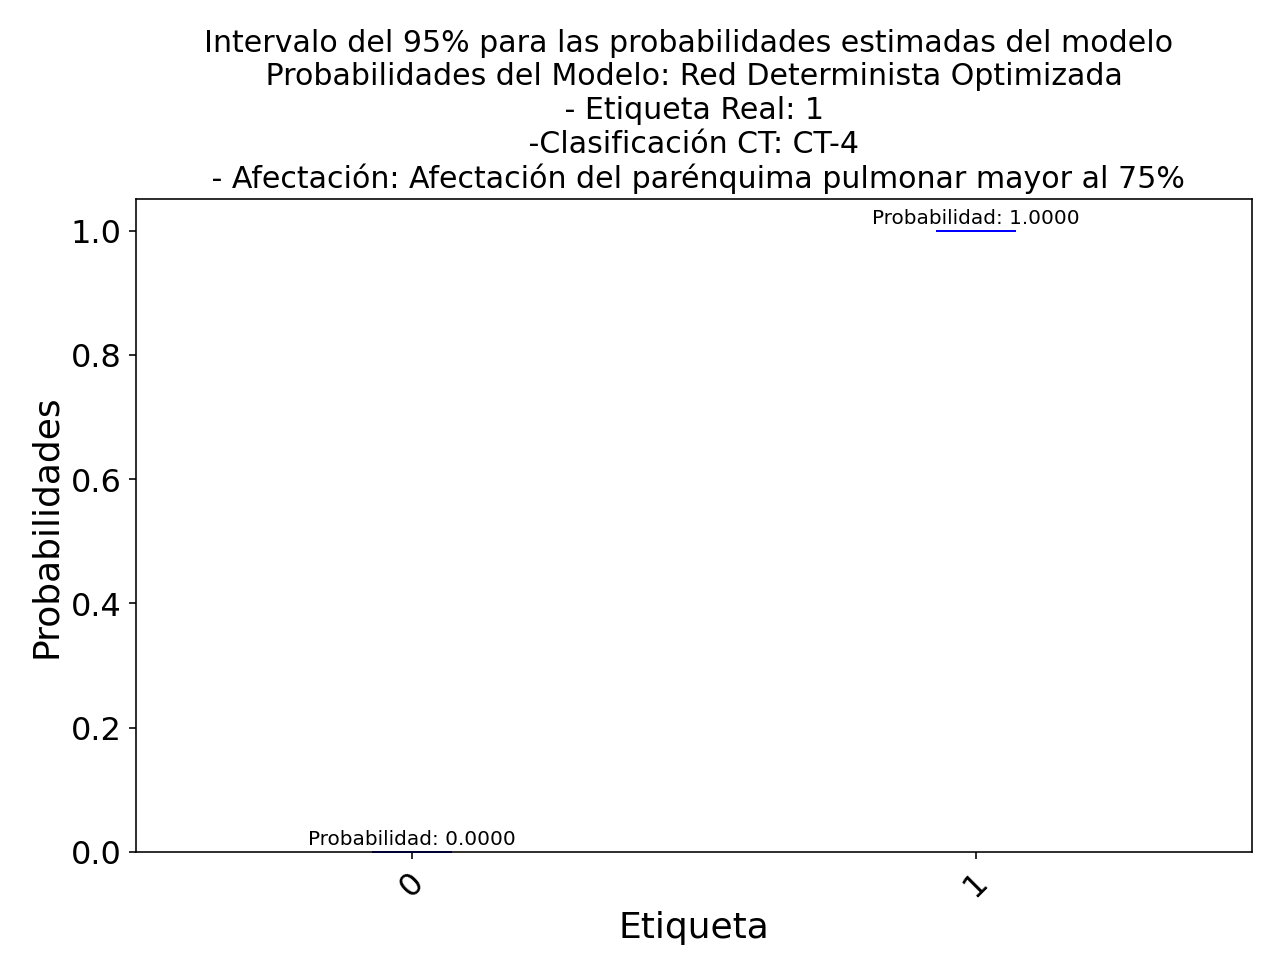
\includegraphics[scale=0.25]{G:/Mi unidad/Maestria/Tesis/Bayesian_NN/Modelos_Colab/Resultados_3D/metricas/4_ct_4_determinista.png}
		\caption{Red Neuronal Determinista}
		\label{fig:4_ct4_2}
	\end{subfigure}
	\hfill
	\begin{subfigure}[b]{0.45\textwidth}
		\centering
		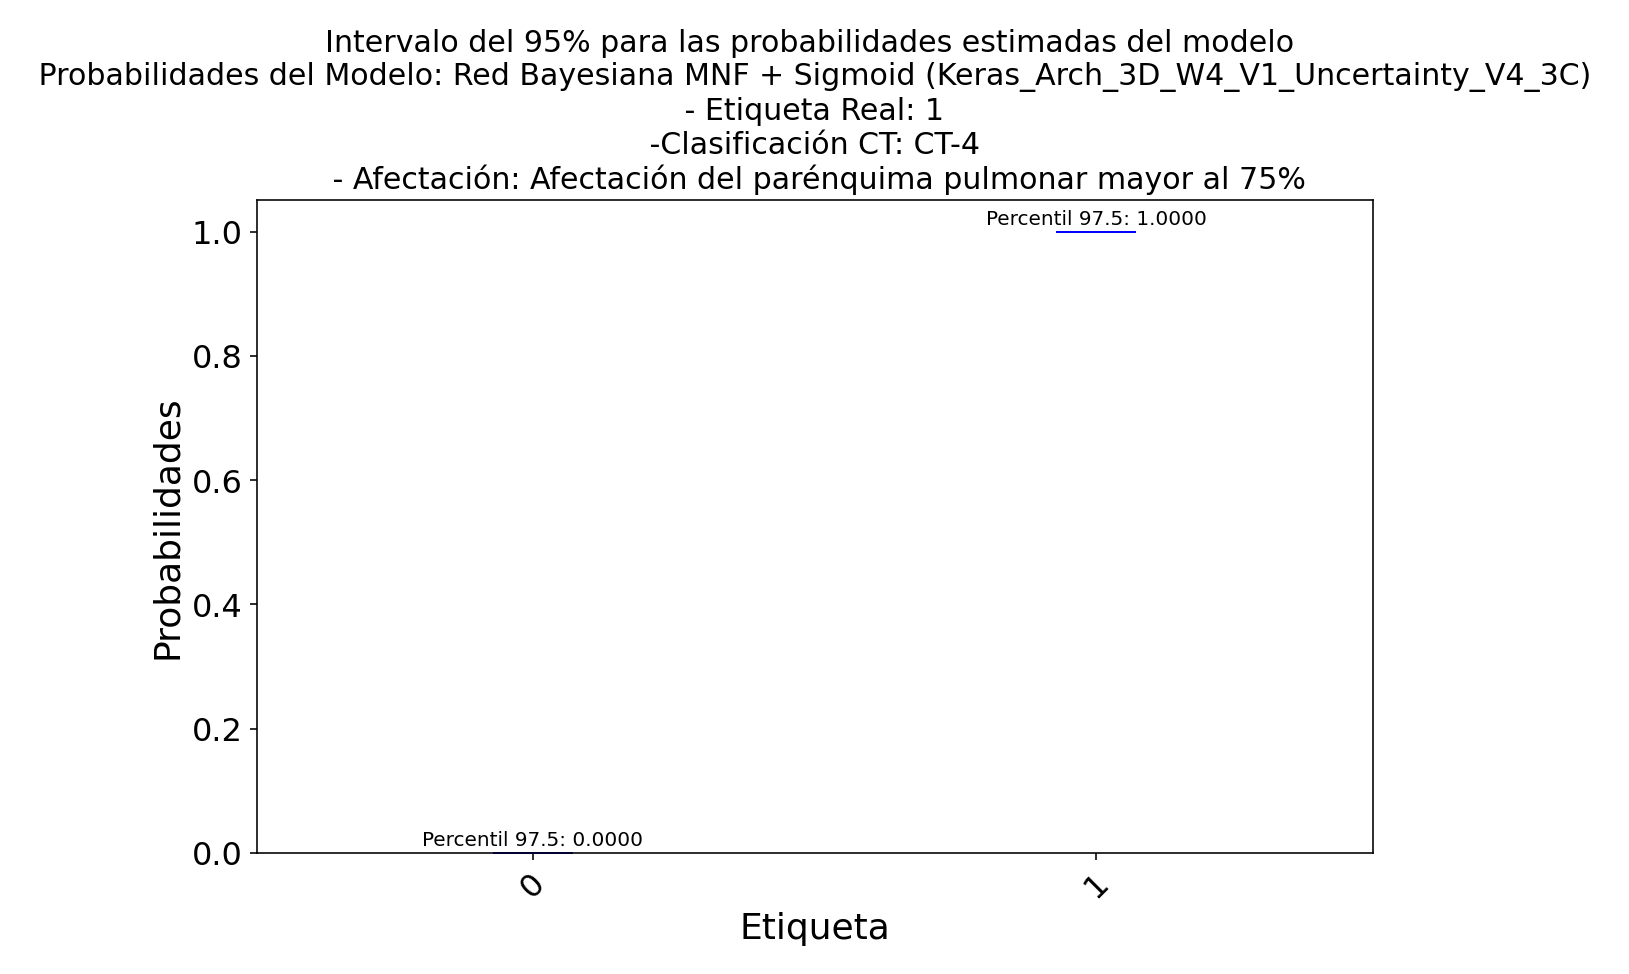
\includegraphics[scale=0.25]{G:/Mi unidad/Maestria/Tesis/Bayesian_NN/Modelos_Colab/Resultados_3D/metricas/4_ct_4_mnf_sigmoid.png}
		\caption{Red Neuronal Bayesiana}
		\label{fig:4_ct4_3}
	\end{subfigure}
	
	\caption{Análisis Incertidumbre - Imagen 4: CT-4}
	\label{fig:layout_4}
\end{figure}
	
	\end{itemize}
	
	\item Imágenes de clase CT-0:
	
	\begin{itemize}
	\item Imagen 5 (Fig.(~\ref{fig:layout_5})): El modelo determinista exhibió un sesgo hacia la etiqueta 1, mientras que el modelo bayesiano se inclinó hacia la etiqueta 0. A pesar de que la etiqueta real era 0 (ausencia de anomalías), los amplios intervalos de predicción del modelo bayesiano indican una incertidumbre sustancial. La presencia de estos amplios intervalos de predicción en el modelo bayesiano sugiere que el modelo no está completamente seguro de su predicción, abriendo una alerta para un diagnóstico clínico más detallado. Esto resalta la importancia de las redes neuronales bayesianas en el campo de la medicina, ya que proporcionan información crucial sobre la incertidumbre asociada con las predicciones, lo que puede ayudar a los profesionales médicos a tomar decisiones más informadas y precisas.
	Los intervalos de confianza para cada clase por el modelo bayesiano son:
	\begin{itemize}
	\item Clase 0: [0.27592939 - 0.98892005] 
	\item Clase 1: [0.01107995 - 0.72407061]
	\end{itemize}

\begin{figure}[H]
	\centering
	\begin{subfigure}[b]{0.6\textwidth}
		\centering
		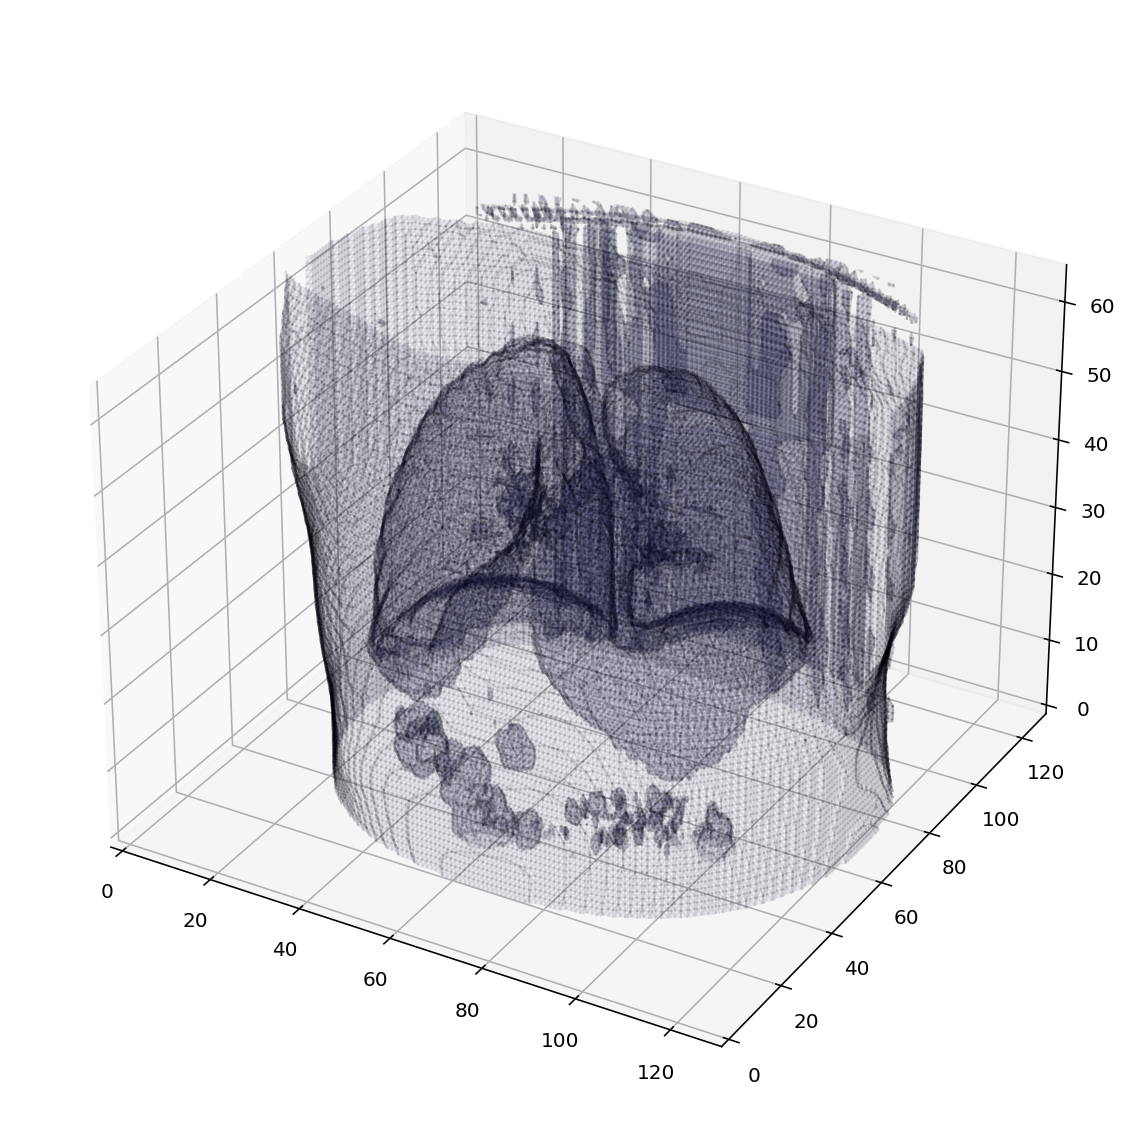
\includegraphics[width=0.5\textwidth]{G:/Mi unidad/Maestria/Tesis/Bayesian_NN/Modelos_Colab/Resultados_3D/metricas/5_ct_0.png} % Adjust the width as needed
		\caption{Representación 3D Tomografía}
		\label{fig:5_ct0_1}
	\end{subfigure}
	
	\medskip
	
	\begin{subfigure}[b]{0.45\textwidth}
		\centering
		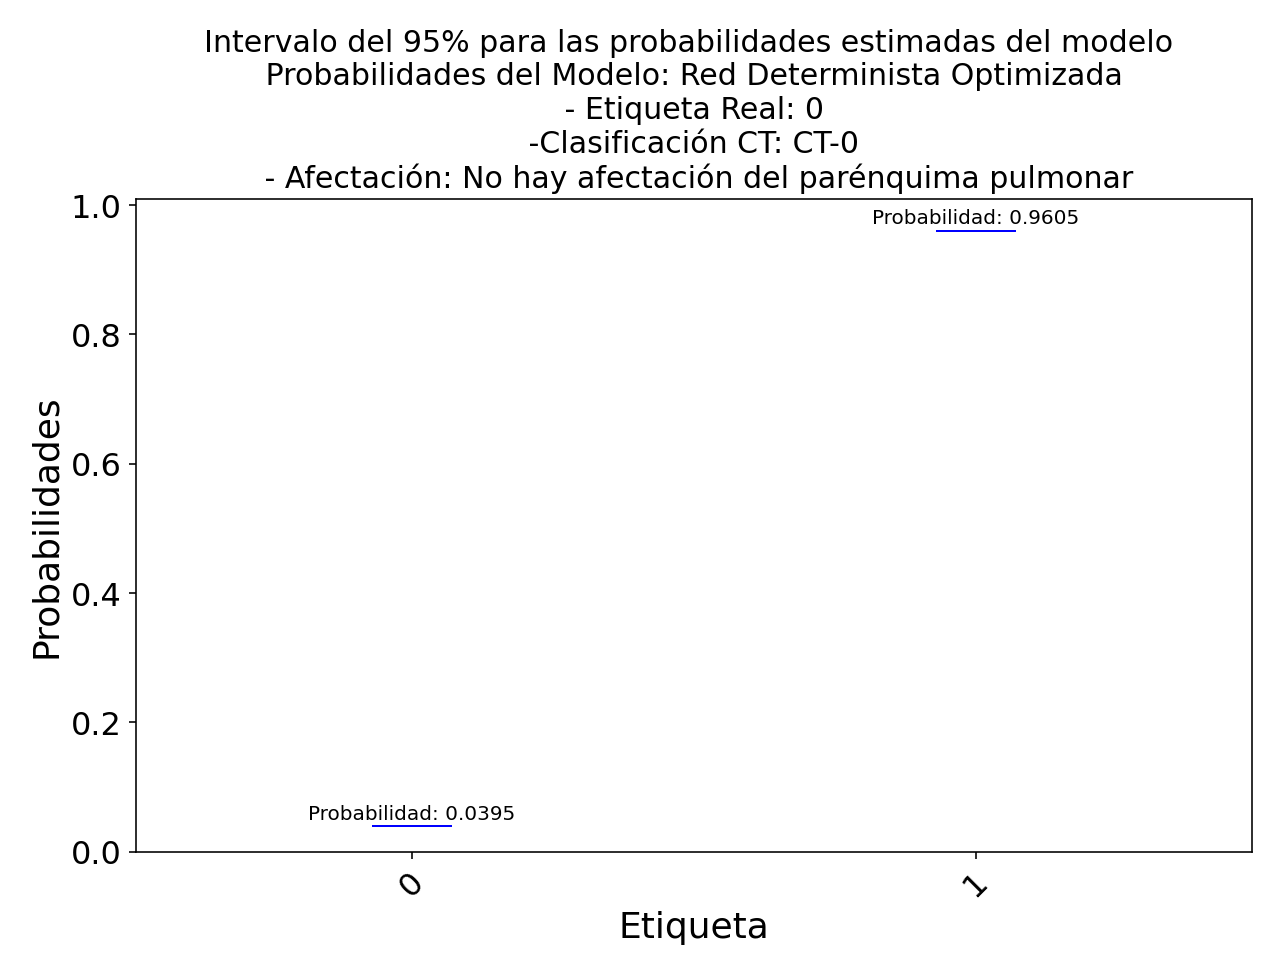
\includegraphics[scale=0.25]{G:/Mi unidad/Maestria/Tesis/Bayesian_NN/Modelos_Colab/Resultados_3D/metricas/5_ct_0_determinista.png}
		\caption{Red Neuronal Determinista}
		\label{fig:5_ct0_2}
	\end{subfigure}
	\hfill
	\begin{subfigure}[b]{0.45\textwidth}
		\centering
		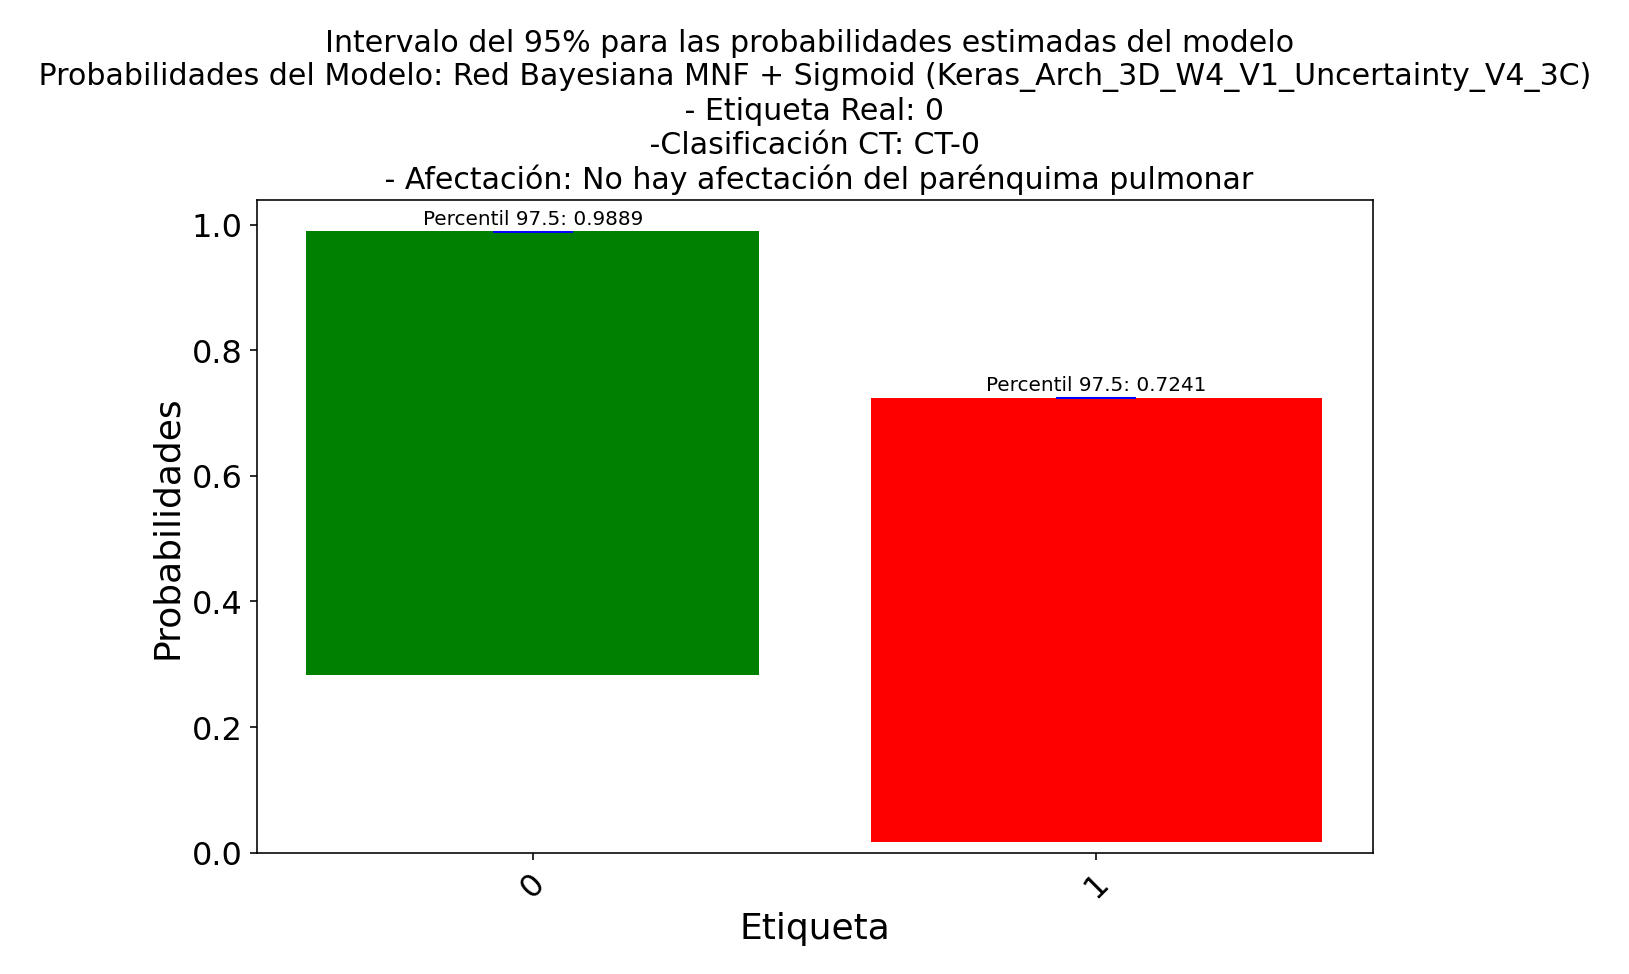
\includegraphics[scale=0.25]{G:/Mi unidad/Maestria/Tesis/Bayesian_NN/Modelos_Colab/Resultados_3D/metricas/5_ct_0_mnf_sigmoid.png}
		\caption{Red Neuronal Bayesiana}
		\label{fig:5_ct0_3}
	\end{subfigure}
	
	\caption{Análisis Incertidumbre - Imagen 5: CT-0}
	\label{fig:layout_5}
\end{figure}
	
	\item Imagen 6 (Fig.(~\ref{fig:layout_6})): Ambos modelos identificaron con precisión la ausencia de anomalías en la tomografía analizada, clasificándola como clase 0. Sin embargo, cabe destacar que el modelo bayesiano muestra intervalos de confianza angostos, indicador de una baja incertidumbre en sus predicciones. Esta característica del modelo bayesiano sugiere una mayor confiabilidad en sus resultados.
	Los intervalos de confianza para cada clase por el modelo bayesiano son:
	\begin{itemize}
	\item Clase 0: [0.93343621 - 0.99933766] 
	\item Clase 1: [0.00066234 - 0.06656379]
	\end{itemize}

\begin{figure}[H]
	\centering
	\begin{subfigure}[b]{0.6\textwidth}
		\centering
		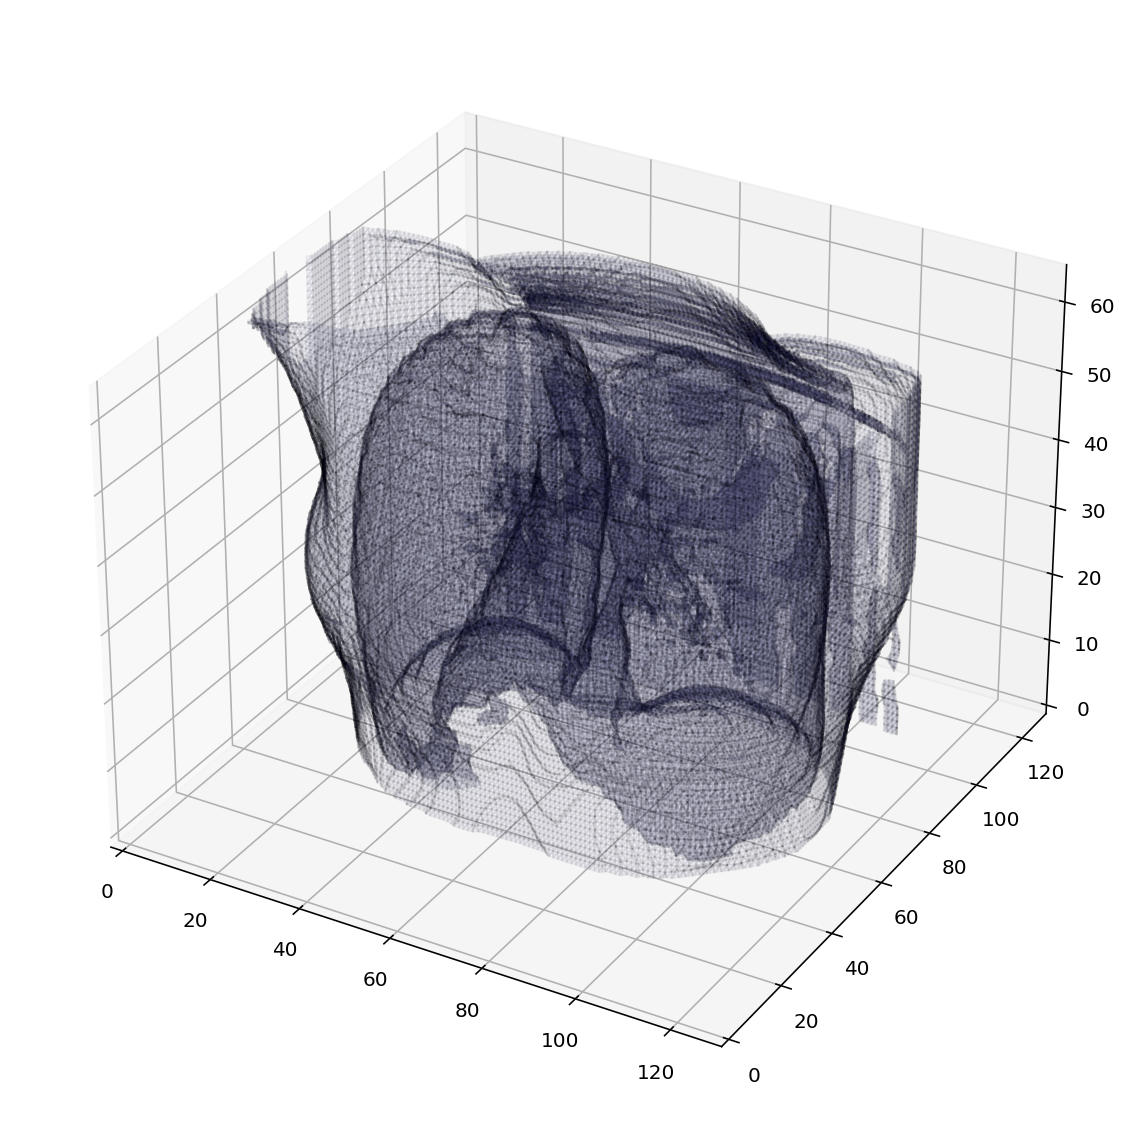
\includegraphics[width=0.5\textwidth]{G:/Mi unidad/Maestria/Tesis/Bayesian_NN/Modelos_Colab/Resultados_3D/metricas/6_ct_0.png} % Adjust the width as needed
		\caption{Representación 3D Tomografía}
		\label{fig:6_ct0_1}
	\end{subfigure}
	
	\medskip
	
	\begin{subfigure}[b]{0.45\textwidth}
		\centering
		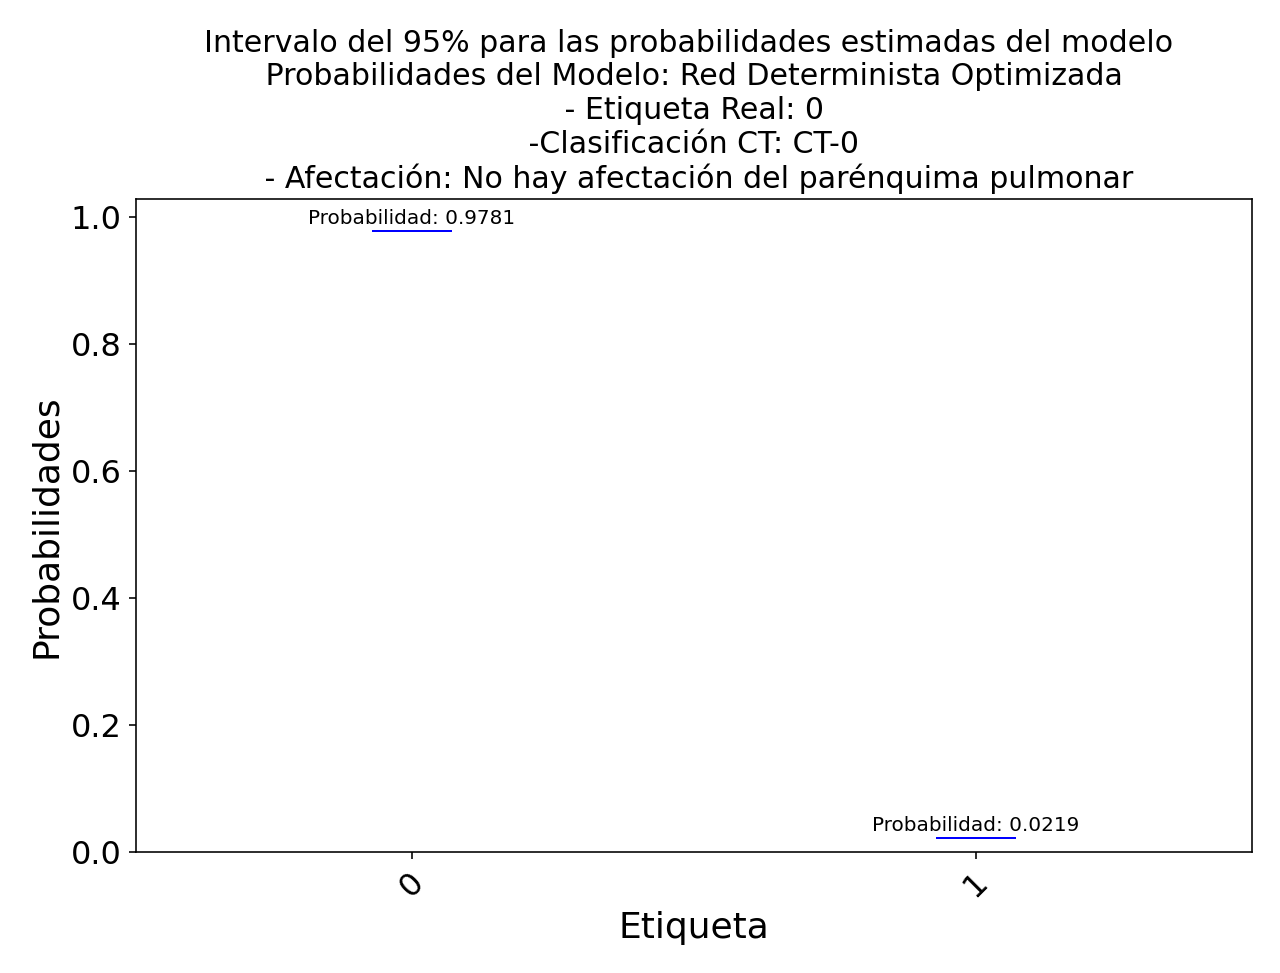
\includegraphics[scale=0.25]{G:/Mi unidad/Maestria/Tesis/Bayesian_NN/Modelos_Colab/Resultados_3D/metricas/6_ct_0_determinista.png}
		\caption{Red Neuronal Determinista}
		\label{fig:6_ct0_2}
	\end{subfigure}
	\hfill
	\begin{subfigure}[b]{0.45\textwidth}
		\centering
		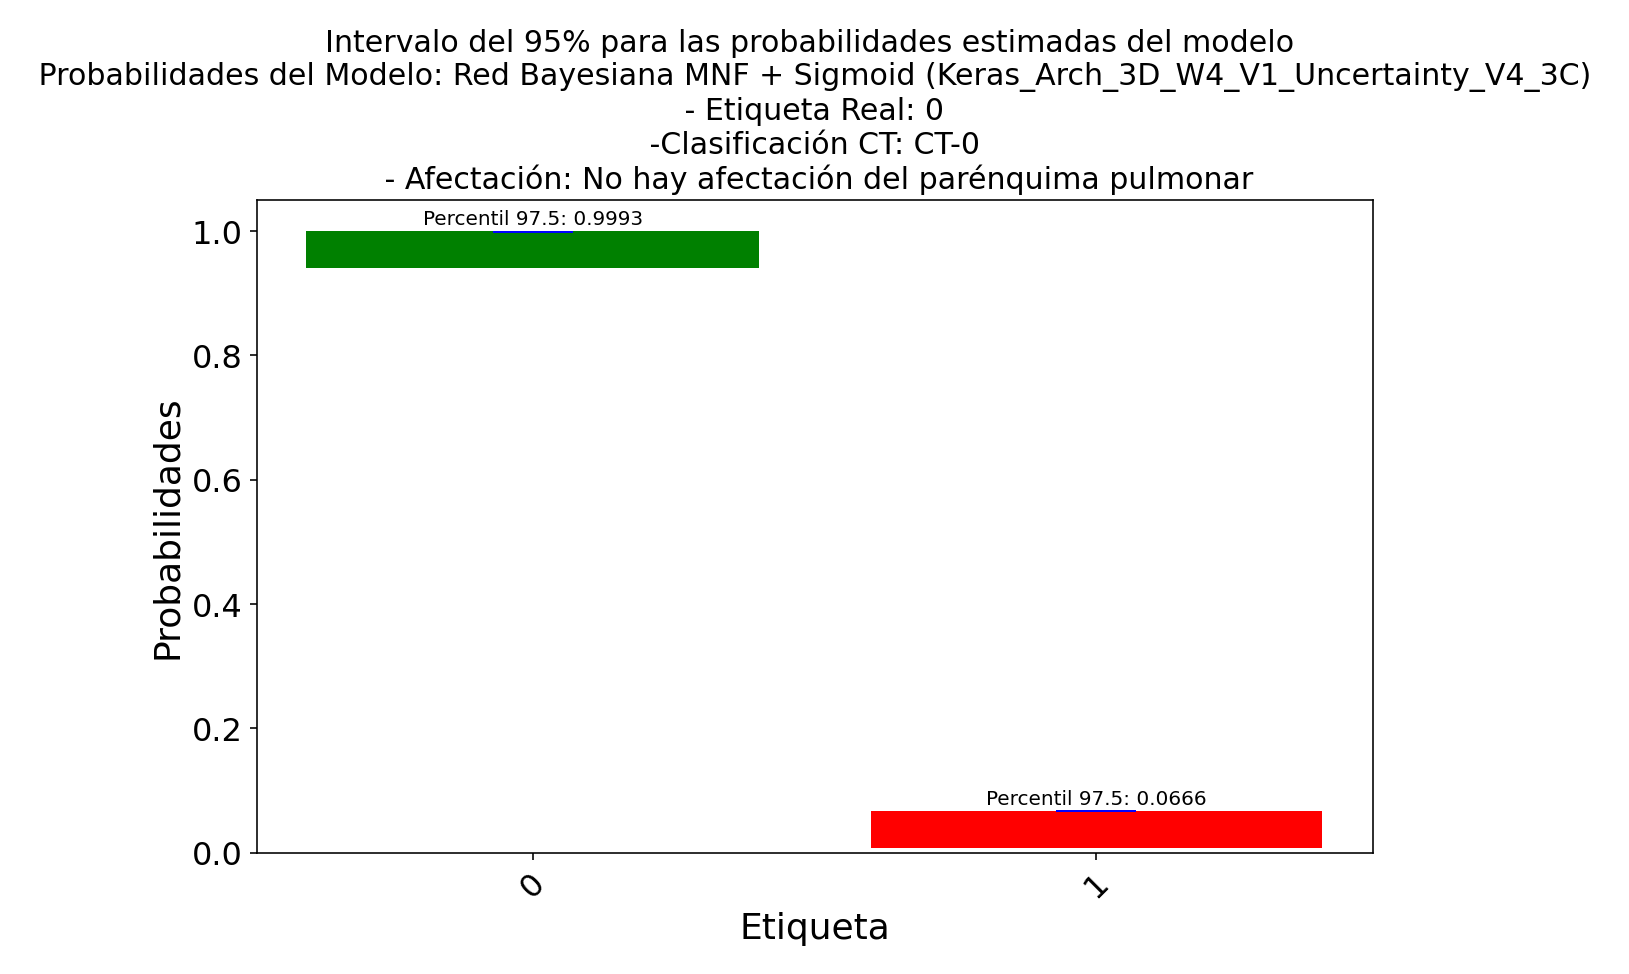
\includegraphics[scale=0.25]{G:/Mi unidad/Maestria/Tesis/Bayesian_NN/Modelos_Colab/Resultados_3D/metricas/6_ct_0_mnf_sigmoid.png}
		\caption{Red Neuronal Bayesiana}
		\label{fig:6_ct0_3}
	\end{subfigure}
	
	\caption{Análisis Incertidumbre - Imagen 6: CT-0}
	\label{fig:layout_6}
\end{figure}
	
	\end{itemize}
	
	
	\end{itemize}
	
	El análisis de imágenes individuales proporciona información sobre el rendimiento predictivo y las capacidades de estimación de la incertidumbre de los modelos, destacando la importancia de la conciencia de la incertidumbre en los procesos de toma de decisiones.
	
	El análisis destaca la importancia de la estimación de la incertidumbre en las predicciones de los modelos. A pesar de las imprecisiones del modelo, los amplios intervalos de predicción proporcionados por la red bayesiana en algunas imágenes resaltaron la presencia de incertidumbre en las predicciones. Este reconocimiento de la incertidumbre es crucial para los procesos de toma de decisiones, ya que alerta a las partes interesadas sobre las ''dudas'' del modelo sobre ciertas predicciones y fomenta una interpretación cautelosa de los resultados.
	
	Es importante destacar que intervalos excepcionalmente anchos en las predicciones de la red bayesiana pueden servir como señal para despertar alertas y promover una evaluación más detallada por parte de los profesionales médicos.
	
	
	\subsection{Tomografías 2D:} \label{resultados_2d}
	
	\subsubsection{Modelos:} \label{r_modelos_2d}
	
	En este capítulo profundizamos en la evaluación de varios modelos entrenados, abarcando enfoques tanto deterministas como bayesianos. Después de ejecutar varias alternativas y entrenar diferentes modelos, incluidos enfoques deterministas y bayesianos, los resultados obtenidos no fueron satisfactorios. Parece que cambiar el tamaño de las tomografías de 3D a 2D puede haber provocado la pérdida de información crucial, afectando negativamente el rendimiento del modelo. En consecuencia, decidimos no continuar con el análisis de calibración e incertidumbre para estos modelos. El gráfico de coordenadas paralelas en la Fig.(~\ref{fig:modelos_2d}) proporciona una representación visual del rendimiento de todos los modelos entrenados:
	
	\begin{figure}[H]
	\centering
	\includegraphics[scale=0.5]{G:/Mi unidad/Maestria/Tesis/Bayesian_NN/Modelos_Colab/Resultados_3D/metricas/2D_Models_test.png}
	\caption{Contaste de métricas evaluadas en los modelos para tomografías 2D - Set de Test}
	\label{fig:modelos_2d}
	\end{figure}	

	Al analizar el gráfico de coordenadas paralelas, resulta evidente que todos los modelos, independientemente de su arquitectura o metodología de entrenamiento, exhiben patrones de rendimiento similares. Esta uniformidad en los resultados denota la necesidad de un enfoque más matizado en el manejo de la etapa de preprocesamiento de datos, particularmente para mitigar la pérdida de información asociada con la conversión de tomografías 3D a 2D.

%	\subsubsection{Calibración:} \label{r_calibracion_2d}
%
%	\subsubsection{Incertidumbre:} \label{r_incertidumbre_2d}

	\section{Conclusiones} \label{conclusiones}
	
	\begin{itemize}
		\item La investigación inicial de las ventanas de la Unidad Hounsfield (HU) proporcionó información valiosa sobre la selección de alternativas de píxeles óptimas para mejorar la discernibilidad de características relevantes durante el entrenamiento de modelos de clasificación. Este paso inicial sentó una base sólida para el posterior desarrollo y optimización del modelo.
		
		\item La optimización de los hiperparámetros dentro de redes deterministas contribuyó significativamente a mejorar las métricas evaluadas, lo que en última instancia nos guió hacia la identificación de una arquitectura óptima para los ejercicios de modelado bayesiano. Este proceso iterativo resaltó la importancia de ajustar los parámetros del modelo para lograr un rendimiento superior.
		
		\item La implementación de arquitecturas bayesianas, en particular aprovechando MNF, demostró ser fundamental para identificar un modelo óptimo capaz de capturar y cuantificar la incertidumbre. Este aspecto es crucial para mejorar la interpretabilidad y confiabilidad de las predicciones de los modelos, especialmente en aplicaciones de atención médica.
		
		\item El análisis de calibración proporcionó información valiosa para comprender la calibración de nuestros modelos, arrojando conocimiento sobre la alineación entre las probabilidades previstas y los resultados reales. Este análisis profundizó nuestra comprensión de la confianza y confiabilidad del modelo.
		
		\item La exploración de la incertidumbre, particularmente a través de los intervalos de confianza generados por las predicciones de los modelos, surgió como un aspecto crítico en la evaluación de la confiabilidad de las predicciones de los modelos. Esta idea es particularmente pertinente en contextos sanitarios, donde las consecuencias de los errores de predicción pueden tener implicaciones importantes. %La integración de mecanismos de cuantificación de la incertidumbre, ejemplificados por la generación de intervalos de confianza durante las predicciones, surgió como una vía fundamental de investigación. Esta nueva comprensión del papel de la incertidumbre adquiere una mayor importancia en los entornos sanitarios, donde la toma de decisiones informadas depende en gran medida de la fiabilidad y confianza de los modelos predictivos.
		
		\item El rendimiento deficiente de los modelos en diversas métricas subraya las limitaciones de la proyección 2D en comparación con la tomografía 3D. El rendimiento inferior sugiere que las representaciones 3D preservan información vital crítica para predicciones precisas, destacando la superioridad de la tomografía 3D sobre las proyecciones 2D para nuestra tarea de clasificación.
		
		\item Las metodologías y los conocimientos obtenidos de este estudio ejemplifican la utilidad de las técnicas de aprendizaje profundo en aplicaciones sanitarias. Al ofrecer enfoques matizados para el análisis de datos y la cuantificación de la incertidumbre, estos hallazgos resaltan el potencial transformador del aprendizaje profundo en el avance de las imágenes médicas y la mejora de los procesos de toma de decisiones clínicas. Estos avances sirven como testimonio de las invaluables contribuciones de las metodologías de aprendizaje profundo para abordar desafíos complejos de atención médica y mejorar los resultados de la atención al paciente.
	\end{itemize}
	
	En conclusión, este proyecto se adentró en el ámbito de la clasificación de la neumonía COVID-19 en tomografías computarizadas 3D utilizando arquitecturas de redes neuronales tanto bayesianas como deterministas. Mediante una experimentación meticulosa, la exploración de hiperparámetros y un análisis de la calibración y la incertidumbre del modelo, se obtuvieron valiosos conocimientos sobre el rendimiento y la fiabilidad de los modelos implementados.

	Mientras que las tomografías tridimensionales arrojaron resultados prometedores, el rendimiento de los modelos entrenados en proyecciones bidimensionales fue menos satisfactorio, lo que indica que las representaciones tridimensionales pueden captar más información crítica para una clasificación precisa.

	Las conclusiones y resultados de este proyecto, junto con los modelos entrenados, están disponibles en el repositorio GitHub \href{https://github.com/juanfierro94/ct-scan-modeling-thesis-bayesian-deterministic}{ct-scan-modeling-thesis-bayesian-deterministic}.

		
	\newpage	
	%\bibliographystyle{acm}
	%\bibliographystyle{unsrt}
	\bibliographystyle{apalike}
	\bibliography{main}
	
	\newpage
	\section{ABREVIACIONES}
	
	\begin{itemize}
		\item NN: Red Neuronal (NN; Neural Network, por sus siglas en inglés) 
		\item DNN: Red Neuronal Profunda (DNN; Deep Neural Network, por sus siglas en inglés)
		\item BNN: Red Neuronal Bayesiana (BNN, Bayesian Neural Network, por sus siglas en inglés)
		\item MNF: Flujos de normalización multiplicativos (MNF; Multiplicative Normalizing Flows, por sus siglas en inglés.)
		\item CNN: Red Neuronal Convolucional (CNN, Convolutional Neural Network, por sus siglas en inglés)
	\end{itemize}
	
	\newpage
	
	\appendix
	\section{ANEXOS}


	\subsection{Descripción modelos evaluados} \label{anexo_tabla_modelos}
	
	Las tablas relacionadas en este anexo describen brevemente el detalle de cada modelo implementado durante el proyecto.
	
\begin{table}[H]
	\resizebox{\textwidth}{!}{%
		\begin{tabular}{|c|c|c|c|p{0.4\linewidth}|c|c|c|c|}
			\hline
			\textbf{Nombre   Modelo} & \textbf{Nombre del   notebook} & \textbf{Dimensión} & \textbf{Tipo} & \textbf{Descripción} & \textbf{Ventana} & \textbf{Tasa de   Aprendizaje} & \textbf{Épocas} & \textbf{Batch Size} \\ \hline
			Keras\_Arch\_3D\_W1\_V1 & 2\_W1\_Modelo\_V1.ipynb & 3D & Determinista & Modelo   con arquitectura tomada del ejercicio de Keras paras redes neuronales 3D. & W1 & 0,001 & 100 & 2 \\ \hline
			Keras\_Arch\_3D\_W1\_V2 & 2\_W1\_Modelo\_V2.ipynb & 3D & Determinista & Modelo   con arquitectura tomada del ejercicio de Keras paras redes neuronales 3D +   Implementación de técnicas de Data Augmentation & W1 & 0,0001 & 100 & 2 \\ \hline
			Resnet18\_Arch\_3D\_W1\_V4 & 2\_W1\_Modelo\_V4.ipynb & 3D & Determinista & Implementación   del modelo Resnet18 del paquete classification\_models\_3D y añadiendo una capa   GlobalMaxPooling3D & W1 & 0,0001 & 100 & 2 \\ \hline
			Resnet18\_Arch\_3D\_W1\_V5 & 2\_W1\_Modelo\_V5.ipynb & 3D & Determinista & Implementación   del modelo Resnet18 del paquete classification\_models\_3D y añadiendo una capa   GlobalMaxPooling3D & W1 & 0,001 & 100 & 2 \\ \hline
			Resnet18\_Arch\_3D\_W1\_V6 & 2\_W1\_Modelo\_V6.ipynb & 3D & Determinista & Implementación   del modelo Resnet18 del paquete classification\_models\_3D y añadiendo una capa   GlobalAveragePooling3D & W1 & 0,0001 & 100 & 2 \\ \hline
			Keras\_Arch\_3D\_W2\_V1 & 2\_W2\_Modelo\_V1.ipynb & 3D & Determinista & Modelo   con arquitectura tomada del ejercicio de Keras paras redes neuronales 3D. & W2 & 0,0001 & 100 & 2 \\ \hline
			Keras\_Arch\_3D\_W3\_V1 & 2\_W3\_Modelo\_V1.ipynb & 3D & Determinista & Modelo   con arquitectura tomada del ejercicio de Keras paras redes neuronales 3D. & W3 & 0,0001 & 100 & 2 \\ \hline
			Keras\_Arch\_3D\_W4\_V1 & 2\_W4\_Modelo\_V1.ipynb & 3D & Determinista & Modelo   con arquitectura tomada del ejercicio de Keras paras redes neuronales 3D. & W4 & 0,0001 & 100 & 2 \\ \hline
			Keras\_Arch\_3D\_W4\_V1\_Confirmacion & 2\_W4\_Modelo\_V1\_Confirmado.ipynb & 3D & Determinista & Modelo   con arquitectura tomada del ejercicio de Keras paras redes neuronales 3D. (Se   ejecuta por 2da vez para confirmar valores) & W4 & 0,0001 & 100 & 2 \\ \hline
			Keras\_Arch\_3D\_W4\_V1\_Optimizado & 2\_W4\_Modelo\_V1\_Optimizado.ipynb & 3D & Determinista & Modelo   con arquitectura tomada del ejercicio de Keras paras redes neuronales 3D. +   Optimización con Keras-Tuner & W4 & 0,001 & 60 & 2 \\ \hline
			Keras\_Arch\_3D\_W4\_V1\_Hyper\_Reg & 2\_W4\_Modelo\_V1\_Hiperparametros.ipynb & 3D & Determinista & Modelo Optimizado Determinista + Optimización con Keras-Tuner en términos de Regularizadores & W4 & 0,001 & 60 & 2 \\ \hline
			Resnet18\_Arch\_3D\_W4\_V4 & 2\_W4\_Modelo\_V4.ipynb & 3D & Determinista & Resnet18 & W4 & 0,0001 & 100 & 2 \\ \hline
			Resnet34\_Arch\_3D\_W4\_V5 & 2\_W4\_Modelo\_V5.ipynb & 3D & Determinista & Resnet34 & W4 & 0,0001 & 100 & 2 \\ \hline
			Seresnet18\_Arch\_3D\_W4\_V6 & 2\_W4\_Modelo\_V6.ipynb & 3D & Determinista & Seresnet18 & W4 & 0,0001 & 100 & 2 \\ \hline
			Seresnet34\_Arch\_3D\_W4\_V7 & 2\_W4\_Modelo\_V7.ipynb & 3D & Determinista & Seresnet34 & W4 & 0,0001 & 100 & 2 \\ \hline
			Resnet18\_Arch\_3D\_W4\_V8 & 2\_W4\_Modelo\_V8.ipynb & 3D & Determinista & Resnet18   + Penúltima capa de la arquitectura 3D será GlobalMaxPooling3D & W4 & 0,0001 & 100 & 2 \\ \hline
			Resnet18\_Arch\_3D\_W4\_V9 & 2\_W4\_Modelo\_V9.ipynb & 3D & Determinista & Resnet18   + Penúltima capa de la arquitectura 3D será GlobalMaxPooling3D + Filtros   Modelo 3D: 8 & W4 & 0,0001 & 100 & 2 \\ \hline
			Resnet18\_Arch\_3D\_W4\_V10 & 2\_W4\_Modelo\_V10.ipynb & 3D & Determinista & Resnet18   + Penúltima capa de la arquitectura 3D será GlobalMaxPooling3D + Filtros   Modelo 3D: 16 & W4 & 0,0001 & 100 & 2 \\ \hline
			Resnet18\_Arch\_3D\_W4\_V11 & 2\_W4\_Modelo\_V11.ipynb & 3D & Determinista & Resnet18   + Penúltima capa de la arquitectura 3D será GlobalMaxPooling3D + Filtros   Modelo 3D: 32 & W4 & 0,0001 & 100 & 2 \\ \hline
			Resnet18\_Arch\_3D\_W4\_V12 & 2\_W4\_Modelo\_V12.ipynb & 3D & Determinista & Resnet18   + Penúltima capa de la arquitectura 3D será GlobalMaxPooling3D + Filtros   Modelo 3D: 8 & W4 & 0,0001 & 100 & 6 \\ \hline
			Resnet18\_Arch\_3D\_W4\_V13 & 2\_W4\_Modelo\_V13.ipynb & 3D & Determinista & Resnet18   + Penúltima capa de la arquitectura 3D será GlobalMaxPooling3D & W4 & 0,0001 & 100 & 4 \\ \hline
			Resnet34\_Arch\_3D\_W4\_V14 & 2\_W4\_Modelo\_V14.ipynb & 3D & Determinista & Resnet34   + Penúltima capa de la arquitectura 3D será GlobalMaxPooling3D & W4 & 0,0001 & 100 & 4 \\ \hline
			Seresnet18\_Arch\_3D\_W4\_V15 & 2\_W4\_Modelo\_V15.ipynb & 3D & Determinista & Seresnet18   + Penúltima capa de la arquitectura 3D será GlobalMaxPooling3D & W4 & 0,0001 & 100 & 4 \\ \hline
			Seresnet34\_Arch\_3D\_W4\_V16 & 2\_W4\_Modelo\_V16.ipynb & 3D & Determinista & Seresnet34   + Penúltima capa de la arquitectura 3D será GlobalMaxPooling3D & W4 & 0,0001 & 100 & 2 \\ \hline
			Efficientnetb0\_Arch\_3D\_W4\_V17 & 2\_W4\_Modelo\_V17.ipynb & 3D & Determinista & Efficientnetb0   + Penúltima capa de la arquitectura 3D será GlobalMaxPooling3D & W4 & 0,0001 & 100 & 2 \\ \hline
			Densenet121\_Arch\_3D\_W4\_V18 & 2\_W4\_Modelo\_V18.ipynb & 3D & Determinista & Densenet121   + Penúltima capa de la arquitectura 3D será GlobalMaxPooling3D & W4 & 0,0001 & 100 & 2 \\ \hline
			Keras\_Arch\_3D\_W4\_V1\_Uncertainty\_V1 & 2\_W4\_Modelo\_V1\_Uncertainty\_V1.ipynb & 3D & Bayesiano & Keras   (Optimizado Tuner) + Capa Bernoulli || NO TIENE MÉTRICAS & W4 & 0,001 & 150 & 2 \\ \hline
			Keras\_Arch\_3D\_W4\_V1\_Uncertainty\_V2 & 2\_W4\_Modelo\_V1\_Uncertainty\_V2.ipynb & 3D & Bayesiano & Keras   (Optimizado Tuner) + Capa Bernoulli (MEAN) || NO TIENE MÉTRICAS & W4 & 0,001 & 150 & 2 \\ \hline
			Keras\_Arch\_3D\_W4\_V1\_Uncertainty\_V2\_2 & 2\_W4\_Modelo\_V1\_Uncertainty\_V2\_2.ipynb & 3D & Bayesiano & Keras   (Optimizado Tuner) + Capa Bernoulli (MEAN) & W4 & 0,0001 & 300 & 2 \\ \hline
			Keras\_Arch\_3D\_W4\_V1\_Uncertainty\_V3 & 2\_W4\_Modelo\_V1\_Uncertainty\_V3.ipynb & 3D & Bayesiano & Keras   (Optimizado Tuner) + Capa MNFDense    Bernoulli || NO TIENE MÉTRICAS & W4 & 0,001 & 150 & 2 \\ \hline
			Keras\_Arch\_3D\_W4\_V1\_Uncertainty\_V4 & 2\_W4\_Modelo\_V1\_Uncertainty\_V4.ipynb & 3D & Bayesiano & Keras   (Optimizado Tuner) + Capa MNFDense    Bernoulli (MEAN) || NO TIENE MÉTRICAS & W4 & 0,001 & 150 & 2 \\ \hline
			Keras\_Arch\_3D\_W4\_V1\_Uncertainty\_V4\_2 & 2\_W4\_Modelo\_V1\_Uncertainty\_V4\_2.ipynb & 3D & Bayesiano & Keras   (Optimizado Tuner) + Capa MNFDense    Bernoulli (MEAN) & W4 & 0,0001 & 800 & 2 \\ \hline
			Keras\_Arch\_3D\_W4\_V1\_Uncertainty\_V4\_2C & 2\_W4\_Modelo\_V1\_Uncertainty\_V4\_2C.ipynb & 3D & Bayesiano & Keras   (Optimizado Tuner) + Capa MNFDense    Bernoulli (MEAN) | Es el mismo modelo V4\_2, solo que se ejecutó   nuevamente porque los pesos guardados del original estaban corruptos & W4 & 0,0001 & 800 & 2 \\ \hline
			Keras\_Arch\_3D\_W4\_V1\_Uncertainty\_V5 & 2\_W4\_Modelo\_V1\_Uncertainty\_V5.ipynb & 3D & Bayesiano & Keras   (Optimizado Tuner) + Capa DenseFlipout Bernoulli (MEAN) & W4 & 0,0001 & 300 & 2 \\ \hline
			Keras\_Arch\_3D\_W4\_V1\_Uncertainty\_V6 & 2\_W4\_Modelo\_V1\_Uncertainty\_V6.ipynb & 3D & Bayesiano & Keras   (Optimizado Tuner) + Capa DenseLocalReparameterization Bernoulli (MEAN) & W4 & 0,0001 & 300 & 2 \\ \hline
			Keras\_Arch\_3D\_W4\_V1\_Uncertainty\_V7 & 2\_W4\_Modelo\_V1\_Uncertainty\_V7.ipynb & 3D & Bayesiano & Keras   (Optimizado Tuner) + Capa DenseReparameterization Bernoulli (MEAN) & W4 & 0,0001 & 300 & 2 \\ \hline
			Keras\_Arch\_3D\_W4\_V1\_Uncertainty\_V4\_3 & 2\_W4\_Modelo\_V1\_Uncertainty\_V4\_3.ipynb & 3D & Bayesiano & Keras   (Optimizado Tuner) + Capa MNFDense    Bernoulli (MEAN) + Capas MNFConv3D & W4 & 0,0001 & 300 & 2 \\ \hline
			Keras\_Arch\_3D\_W4\_V1\_Uncertainty\_V4\_3C & 2\_W4\_Modelo\_V1\_Uncertainty\_V4\_3C.ipynb & 3D & Bayesiano & Keras   (Optimizado Tuner) + Capa MNFDense    Bernoulli (MEAN) + Capas MNFConv3D | Es el mismo modelo V4\_3, solo que   se ejecutó nuevamente porque los pesos guardados del original estaban   corruptos & W4 & 0,0001 & 300 & 2 \\ \hline
			Keras\_Arch\_3D\_W4\_V1\_Uncertainty\_MCDropout & 2\_W4\_Modelo\_V1\_Optimizado\_MCDropout.ipynb & 3D & Bayesiano & Keras   (Optimizado Tuner) + Dropout MC & W4 & 0,0001 & 100 & 2 \\ \hline
			Keras\_Arch\_3D\_W4\_V1\_Uncertainty\_V8 & 2\_W4\_Modelo\_V1\_Uncertainty\_V8.ipynb & 3D & Bayesiano & Keras   (Optimizado Tuner) + Capa DenseFlipout Bernoulli (MEAN) + Capas ConvFlipout & W4 & 0,0001 & 300 & 2 \\ \hline
			Keras\_Arch\_3D\_W4\_V1\_Uncertainty\_V9 & 2\_W4\_Modelo\_V1\_Uncertainty\_V9.ipynb & 3D & Bayesiano & Keras   (Optimizado Tuner) + Capa DenseReparameterization Bernoulli (MEAN) + Capas   Conv Reparametrization & W4 & 0,0001 & 300 & 2 \\ \hline
		\end{tabular}%
	}
	\caption{Descripción Modelos 3D}
	\label{tab:info_modelos_3D}
\end{table}

% Please add the following required packages to your document preamble:
% \usepackage{graphicx}
\begin{table}[H]
	\resizebox{\textwidth}{!}{%
		\begin{tabular}{|c|c|c|c|p{0.4\linewidth}|c|c|c|c|}
			\hline
			\textbf{Nombre   Modelo} & \textbf{Nombre del   notebook} & \textbf{Dimensión} & \textbf{Tipo} & \textbf{Descripción} & \textbf{Ventana} & \textbf{Tasa de   Aprendizaje} & \textbf{Épocas} & \textbf{Batch Size} \\ \hline
			Keras\_Arch\_W4\_V1\_Optimizado\_2D\_MEAN & 2\_W4\_Modelo\_Keras\_2D\_MEAN.ipynb & 2D & Determinista & Modelo   determinista con arquitectura optimizada    + Conversión imagénes 3D a 2D a través del promedio de los pixeles de   los slices (3ra dimensión). & W4 & 0,0001 & 150 & 2 \\ \hline
			Keras\_Arch\_W4\_V1\_Optimizado\_2D\_MEAN\_V2 & 2\_W4\_Modelo\_Keras\_2D\_MEAN\_V2.ipynb & 2D & Determinista & Modelo   determinista con arquitectura optimizada    + Conversión imagénes 3D a 2D a través del promedio de los pixeles de   los slices (3ra dimensión). & W4 & 0,001 & 150 & 2 \\ \hline
			Keras\_Arch\_W4\_V1\_Optimizado\_2D\_MEAN\_V3 & 2\_W4\_Modelo\_Keras\_2D\_MEAN\_V3.ipynb & 2D & Determinista & Modelo   determinista con arquitectura optimizada    + Conversión imagénes 3D a 2D a través del promedio de los pixeles de   los slices (3ra dimensión). & W4 & 0,00001 & 150 & 2 \\ \hline
			Keras\_Arch\_W4\_V1\_Optimizado\_2D\_MEAN\_V2\_V1 & 2\_W4\_Modelo\_Keras\_2D\_MEAN\_V2\_V1.ipynb & 2D & Determinista & Modelo   determinista con arquitectura optimizada    + Conversión imagénes 3D a 2D a través del promedio de los pixeles de   los slices (3ra dimensión). & W4 & 0,001 & 150 & 4 \\ \hline
			Keras\_Arch\_W4\_V1\_Optimizado\_2D\_MEAN\_V2\_V2 & 2\_W4\_Modelo\_Keras\_2D\_MEAN\_V2\_V2.ipynb & 2D & Determinista & Modelo   determinista con arquitectura optimizada    + Conversión imagénes 3D a 2D a través del promedio de los pixeles de   los slices (3ra dimensión). & W4 & 0,001 & 150 & 8 \\ \hline
			Keras\_Arch\_W4\_V1\_Optimizado\_2D\_SUM & 2\_W4\_Modelo\_Keras\_2D\_SUM.ipynb & 2D & Determinista & Modelo   determinista con arquitectura optimizada    + Conversión imagénes 3D a 2D a través de la suma de los pixeles de   los slices (3ra dimensión). & W4 & 0,0001 & 150 & 2 \\ \hline
			Keras\_Arch\_W4\_V1\_Optimizado\_2D\_MAX & 2\_W4\_Modelo\_Keras\_2D\_MAX.ipynb & 2D & Determinista & Modelo   determinista con arquitectura optimizada    + Conversión imagénes 3D a 2D a través del máximo de los pixeles de   los slices (3ra dimensión). & W4 & 0,0001 & 150 & 2 \\ \hline
			MNF\_Arch\_W4\_V1\_Optimizado\_2D\_MEAN & 2\_W4\_Modelo\_MNF\_2D\_MEAN.ipynb & 2D & Bayesiano & Modelo   bayesiano MNF + Conversión imagénes 3D a 2D a través del promedio de los   pixeles de los slices (3ra dimensión). & W4 & 0,0001 & 300 & 2 \\ \hline
			MNF\_Arch\_W4\_V1\_Optimizado\_2D\_MEAN\_V2 & 2\_W4\_Modelo\_MNF\_2D\_MEAN\_V2.ipynb & 2D & Bayesiano & Modelo   bayesiano MNF + Conversión imagénes 3D a 2D a través del promedio de los   pixeles de los slices (3ra dimensión). & W4 & 0,001 & 300 & 2 \\ \hline
			MNF\_Arch\_W4\_V1\_Optimizado\_2D\_MEAN\_V3 & 2\_W4\_Modelo\_MNF\_2D\_MEAN\_V3.ipynb & 2D & Bayesiano & Modelo   bayesiano MNF + Conversión imagénes 3D a 2D a través del promedio de los   pixeles de los slices (3ra dimensión). & W4 & 0,00001 & 300 & 2 \\ \hline
			MNF\_Arch\_W4\_V1\_Optimizado\_2D\_MEAN\_V4 & 2\_W4\_Modelo\_MNF\_2D\_MEAN\_V4.ipynb & 2D & Bayesiano & Modelo   bayesiano MNF + Conversión imagénes 3D a 2D a través del promedio de los   pixeles de los slices (3ra dimensión). & W4 & 0,0001 & 300 & 4 \\ \hline
			MNF\_Arch\_W4\_V1\_Optimizado\_2D\_MEAN\_V5 & 2\_W4\_Modelo\_MNF\_2D\_MEAN\_V5.ipynb & 2D & Bayesiano & Modelo   bayesiano MNF + Conversión imagénes 3D a 2D a través del promedio de los   pixeles de los slices (3ra dimensión). & W4 & 0,0001 & 300 & 8 \\ \hline
			MNF\_Arch\_W4\_V1\_Optimizado\_2D\_SUM & 2\_W4\_Modelo\_MNF\_2D\_SUM.ipynb & 2D & Bayesiano & Modelo   bayesiano MNF + Conversión imagénes 3D a 2D a través de la suma de los   pixeles de los slices (3ra dimensión). & W4 & 0,0001 & 300 & 2 \\ \hline
			MNF\_Arch\_W4\_V1\_Optimizado\_2D\_MAX & 2\_W4\_Modelo\_MNF\_2D\_MAX.ipynb & 2D & Bayesiano & Modelo   bayesiano MNF + Conversión imagénes 3D a 2D a través del máximo de los   pixeles de los slices (3ra dimensión). & W4 & 0,0001 & 300 & 2 \\ \hline
		\end{tabular}%
	}
	\caption{Descripción Modelos 2D}
	\label{tab:info_modelos_2D}
\end{table}

	\subsection{Cambios Iniciales Transición Determinista - Bayesiana} \label{codigo_bayesiana_1}
	
	El código relacionado en este anexo comprende los cambios realizados a la arquitectura del modelo determinista para iniciar la transición hacia el campo bayesiano.
	
	\begin{adjustbox}{max width=\textwidth}
	\begin{lstlisting}[language=Python, caption={Capa Final - Modelo determinista:}]
		outputs = layers.Dense(units=1, activation="sigmoid")(x)
	\end{lstlisting}
	\end{adjustbox}

	\begin{adjustbox}{max width=\textwidth}
	\begin{lstlisting}[language=Python, caption={Alternativa para Modelo Bayesiano:}]
		# Opcion 1 - A
		x = layers.Dense(units=tfp.layers.IndependentBernoulli.params_size(1))(x)
		outputs = tfp.layers.IndependentBernoulli(1)(x)
		
		# Opcion 1 - B
		x = layers.Dense(units=tfp.layers.IndependentBernoulli.params_size(1))(x)
		outputs = tfp.layers.IndependentBernoulli(1, tfd.Bernoulli.mean)(x)
		
		# Opcion 2 - A
		x = MNFDense(tfp.layers.IndependentBernoulli.params_size(1))(x)
		outputs = tfp.layers.IndependentBernoulli(1)(x)
		
		# Opcion 2 - B
		x = MNFDense(tfp.layers.IndependentBernoulli.params_size(1))(x)
		outputs = tfp.layers.IndependentBernoulli(1, tfd.Bernoulli.mean)(x)
	\end{lstlisting}
	\end{adjustbox}

	\subsection{Métricas Primeras Alternativas Redes Bayesianas} \label{metricas_bayesiana_1}
	
	Las gráficas relacionadas en este anexo comprenden la evolución época a época del entrenamiento de los primeros modelos bayesianos.
	
	\begin{figure}[H]
	\centering
	\includegraphics[scale=0.3]{G:/Mi unidad/Maestria/Tesis/Bayesian_NN/Modelos_Colab/Resultados_3D/metricas/bayesian_1a.png}
	\caption{Evolución Red Neuronal Bayesiana - Opción 1A}
	\label{fig:bayesian_1}
	\end{figure}
	
	\begin{figure}[H]
		\centering
		\includegraphics[scale=0.3]{G:/Mi unidad/Maestria/Tesis/Bayesian_NN/Modelos_Colab/Resultados_3D/metricas/bayesian_1b.png}
		\caption{Evolución Red Neuronal Bayesiana - Opción 1B}
		\label{fig:bayesian_2}
	\end{figure}
	
	\begin{figure}[H]
		\centering
		\includegraphics[scale=0.3]{G:/Mi unidad/Maestria/Tesis/Bayesian_NN/Modelos_Colab/Resultados_3D/metricas/bayesian_2a.png}
		\caption{Evolución Red Neuronal Bayesiana - Opción 2A}
		\label{fig:bayesian_3}
	\end{figure}
	
	\begin{figure}[H]
		\centering
		\includegraphics[scale=0.3]{G:/Mi unidad/Maestria/Tesis/Bayesian_NN/Modelos_Colab/Resultados_3D/metricas/bayesian_2b.png}
		\caption{Evolución Red Neuronal Bayesiana - Opción 2B}
		\label{fig:bayesian_4}
	\end{figure}

	\subsection{Monte Carlo Dropout} \label{Monte_Carlo_Dropout}

	El código relacionado en este anexo comprende los cambios realizados a la arquitectura del modelo determinista para entrenar la red bayesiana Monte Carlo Dropout.
	
	\begin{adjustbox}{max width=\textwidth}
	\begin{lstlisting}[language=Python, caption={Arquitectura determinista}]
		def get_model(width=128, height=128, depth=64):
		"""Build a 3D convolutional neural network model."""
		
		inputs = keras.Input((width, height, depth, 1))
		
		x = layers.Conv3D(filters=128, kernel_size=3, activation="relu")(inputs)
		x = layers.MaxPool3D(pool_size=2)(x)
		x = layers.BatchNormalization()(x)
		
		x = layers.Conv3D(filters=128, kernel_size=3, activation="relu")(x)
		x = layers.MaxPool3D(pool_size=2)(x)
		x = layers.BatchNormalization()(x)
		
		x = layers.Conv3D(filters=256, kernel_size=3, activation="relu")(x)
		x = layers.MaxPool3D(pool_size=2)(x)
		x = layers.BatchNormalization()(x)
		
		x = layers.Conv3D(filters=512, kernel_size=3, activation="relu")(x)
		x = layers.MaxPool3D(pool_size=2)(x)
		x = layers.BatchNormalization()(x)
		
		x = layers.GlobalMaxPooling3D()(x)
		x = layers.Dense(units=256, activation="relu")(x)
		x = layers.Dropout(0.2)(x)
		
		outputs = layers.Dense(units=1, activation="sigmoid")(x)
		
		# Define the model.
		model = keras.Model(inputs, outputs, name="3dcnn")
		return model
		
		
		# Build model.
		model = get_model(width=128, height=128, depth=64)
		model.summary()
	\end{lstlisting}
	\end{adjustbox}
	
	
	\begin{lstlisting}[language=Python, caption={Modificamos la capa dropout:}]
		x = layers.Dropout(0.2)(x)
	\end{lstlisting}
	
	\begin{lstlisting}[language=Python, caption={Capa modificada:}]
		x = layers.Dropout(0.2)(x, training = True)
	\end{lstlisting}	

	\subsection{Coordenadas Paralelas - Ajuste Capa Sigmoid} \label{coordenadas_paralelas}

	Las gráficas relacionadas en este anexo comprenden:
	
	Fig.(\ref{fig:calibracion_bernoulli_V4_2C_sigmoid_test}): Impacto en las métricas para la red bayesiana en cuestión luego de cambiar la capa de salida probabilística por una capa \textsl{Sigmoid}.
	
	Fig.(\ref{fig:calibracion_bernoulli_V4_3C_sigmoid_test}): Impacto en las métricas para la red bayesiana en cuestión luego de cambiar la capa de salida probabilística por una capa \textsl{Sigmoid}.
	
	Fig.(\ref{fig:calibracion_bernoulli_V6_sigmoid_test}): Impacto en las métricas para la red bayesiana en cuestión luego de cambiar la capa de salida probabilística por una capa \textsl{Sigmoid}.

		\begin{figure}[H]
		\centering
		\includegraphics[scale=0.5]{G:/Mi unidad/Maestria/Tesis/Bayesian_NN/Modelos_Colab/Resultados_3D/metricas/calibracion_bernoulli_V4_2C_sigmoid_test.png}
		\caption{Contaste de métricas evaluadas en los modelos Bayesianos - Set de Test}
		\label{fig:calibracion_bernoulli_V4_2C_sigmoid_test}
		\end{figure}
	
		\begin{figure}[H]
		\centering
		\includegraphics[scale=0.5]{G:/Mi unidad/Maestria/Tesis/Bayesian_NN/Modelos_Colab/Resultados_3D/metricas/calibracion_bernoulli_V4_3C_sigmoid_test.png}
		\caption{Contaste de métricas evaluadas en los modelos Bayesianos - Set de Test}
		\label{fig:calibracion_bernoulli_V4_3C_sigmoid_test}
		\end{figure}
	
		\begin{figure}[H]
		\centering
		\includegraphics[scale=0.5]{G:/Mi unidad/Maestria/Tesis/Bayesian_NN/Modelos_Colab/Resultados_3D/metricas/calibracion_bernoulli_V6_sigmoid_test.png}
		\caption{Contaste de métricas evaluadas en los modelos Bayesianos - Set de Test}
		\label{fig:calibracion_bernoulli_V6_sigmoid_test}
		\end{figure}	

	\subsection{Coordenadas Paralelas - Ajuste Umbral} \label{coordenadas_paralelas_umbral}
	
		La gráfica relacionada en este anexo comprende el impacto en las métricas para los diferentes modelos bayesianos luego de cambiar el umbral de decisión para la clase 1.
	
		\begin{figure}[H]
		\centering
		\includegraphics[scale=0.5]{G:/Mi unidad/Maestria/Tesis/Bayesian_NN/Modelos_Colab/Resultados_3D/metricas/calibracion_corte_test.png}
		\caption{Contaste de métricas evaluadas en los modelos Bayesianos - Set de Test}
		\label{fig:calibracion_corte_test}
		\end{figure}

	\subsection{Diagramas Confiabilidad} \label{resultados_diagrama_conf}
	
	En este anexo presentamos los diagramas de confiabilidad en el set de datos de test para todos los modelos relacionados en la sección \ref{r_calibracion_3d}.
	
	\begin{figure}[H]
	\centering
	
\includegraphics[scale=0.25]{G:/Mi unidad/Maestria/Tesis/Bayesian_NN/Modelos_Colab/Resultados_3D/calibraciones/imagenes/diagramas_confiabilidad_histograma_test2.png}
	\caption{Diagramas Confiabilidad - Set de Test}
	\label{fig:conf_todos2}
	\end{figure}	
	
	%\makesignature{\aluno}{\orientador}
\end{document}

